\documentclass[12pt,bibliography=oldstyle,DIV=12,parskip=half-]{scrreprt}
\newif\iflatexml\latexmlfalse
\usepackage{xstring}
\newcommand{\includePrueba}[1]{\input{#1}}
\newcommand{\includeFileOrFigure}[1]{%
  \IfBeginWith{#1}{figures/}{%
    \begin{figure}[H]
      \figureStyle
      \StrBefore[2]{#1}{/}[\temp]
      \tikzsetnextfilename{figures/femigracion/femigracion}
\begin{tikzpicture}[
    font=\footnotesize,
    thick
  ]
\usetikzlibrary{positioning,fit,calc,shapes}
\def\nw{1cm}

\makeatletter
\pgfkeys{/pgf/.cd,
  parallelepiped offset x/.initial=2mm,
  parallelepiped offset y/.initial=2mm
}
\pgfdeclareshape{parallelepiped}
{
  \inheritsavedanchors[from=rectangle] % this is nearly a rectangle
  \inheritanchorborder[from=rectangle]
  \inheritanchor[from=rectangle]{north}
  \inheritanchor[from=rectangle]{north west}
  \inheritanchor[from=rectangle]{north east}
  \inheritanchor[from=rectangle]{center}
  \inheritanchor[from=rectangle]{west}
  \inheritanchor[from=rectangle]{east}
  \inheritanchor[from=rectangle]{mid}
  \inheritanchor[from=rectangle]{mid west}
  \inheritanchor[from=rectangle]{mid east}
  \inheritanchor[from=rectangle]{base}
  \inheritanchor[from=rectangle]{base west}
  \inheritanchor[from=rectangle]{base east}
  \inheritanchor[from=rectangle]{south}
  \inheritanchor[from=rectangle]{south west}
  \inheritanchor[from=rectangle]{south east}
  \backgroundpath{
    % store lower right in xa/ya and upper right in xb/yb
    \southwest \pgf@xa=\pgf@x \pgf@ya=\pgf@y
    \northeast \pgf@xb=\pgf@x \pgf@yb=\pgf@y
    \pgfmathsetlength\pgfutil@tempdima{\pgfkeysvalueof{/pgf/parallelepiped offset x}}
    \pgfmathsetlength\pgfutil@tempdimb{\pgfkeysvalueof{/pgf/parallelepiped offset y}}
    \def\ppd@offset{\pgfpoint{\pgfutil@tempdima}{\pgfutil@tempdimb}}
    \pgfpathmoveto{\pgfqpoint{\pgf@xa}{\pgf@ya}}
    \pgfpathlineto{\pgfqpoint{\pgf@xb}{\pgf@ya}}
    \pgfpathlineto{\pgfqpoint{\pgf@xb}{\pgf@yb}}
    \pgfpathlineto{\pgfqpoint{\pgf@xa}{\pgf@yb}}
    \pgfpathclose
    \pgfpathmoveto{\pgfqpoint{\pgf@xb}{\pgf@ya}}
    \pgfpathlineto{\pgfpointadd{\pgfpoint{\pgf@xb}{\pgf@ya}}{\ppd@offset}}
    \pgfpathlineto{\pgfpointadd{\pgfpoint{\pgf@xb}{\pgf@yb}}{\ppd@offset}}
    \pgfpathlineto{\pgfpointadd{\pgfpoint{\pgf@xa}{\pgf@yb}}{\ppd@offset}}
    \pgfpathlineto{\pgfqpoint{\pgf@xa}{\pgf@yb}}
    \pgfpathmoveto{\pgfqpoint{\pgf@xb}{\pgf@yb}}
    \pgfpathlineto{\pgfpointadd{\pgfpoint{\pgf@xb}{\pgf@yb}}{\ppd@offset}}
  }
}
\makeatother


\node[cloud,cloud ignores aspect,draw,,minimum width=1.5*\nw,minimum height=\nw] (internet) {Internet};
\node[parallelepiped,draw,minimum width=\nw,minimum height=.75*\nw,node distance=.6*\nw,below = of internet] (firewall) {Firewall};
\node[arrow box,draw=green,arrow box shaft width=.25*\nw,node distance=.6*\nw,below = of firewall] (frontend) {};
\node[arrow box,draw=blue,arrow box shaft width=.25*\nw,node distance=.6*\nw,right = of frontend] (redir) {};
\node[chamfered rectangle,chamfered rectangle corners=north west,draw=magenta,node distance=2*\nw,minimum width=.6*\nw,minimum height=.6*\nw,right = of redir] (svn) {SVN};
\coordinate (aux) at ($ (redir.south) - (0,.6*\nw) $);
\coordinate (auxfe) at ($ (frontend.south) - (0,.6*\nw) $);

% \tikzstyle{srv}=[cylinder,shape border rotate=90, shape aspect=0.4,minimum height=1.2*\nw,minimum width=0.8*\nw,node distance=.5*\nw]
\tikzstyle{srv}=[minimum height=1.4*\nw,minimum width=0.9*\nw,node distance=0.4*\nw]
\tikzstyle{blue}=[draw=blue]
\tikzstyle{green}=[draw=green]
\tikzstyle{magenta}=[draw=magenta]
\node[blue,srv,node distance=.6*\nw, below = of aux,xshift=-.4*\nw ] (srv1) {srv};
\node[green,srv, below left = of srv1 ] (srv2) {srv};
\node[blue,srv, below right = of srv1 ] (srv3) {srv};
\node[green,srv, above left = of srv2 ] (srv4) {srv};
\node[blue,srv, above right = of srv3 ] (srv5) {srv};
\node[blue,srv, below right = of srv5 ] (srv6) {srv};

\draw[-,blue] (srv1.north)  |- (aux) -- (redir.south);
\draw[-,blue] (srv2.north) |- (aux) -- (redir.south);
\draw[-,blue] (srv3.north) |- (aux) -- (redir.south);
\draw[-,blue] (srv4.north) |- (aux) -- (redir.south);
\draw[-,blue] (srv5.north) |- (aux) -- (redir.south);
\draw[-,blue] (srv6.north) |- (aux) -- (redir.south);
\draw[-,green] (srv2.north) |- (auxfe) -- (frontend.south);
\draw[-,green] (srv4.north) |- (auxfe) -- (frontend.south);

\draw[-,dashed,draw=magenta] (svn.west)  -- (redir.east);
\draw[-] (frontend.north)  -- (firewall.south);
\draw[-,green] (frontend.east)  -- (redir.west);
\draw[-] (firewall.north)  -- (internet.south);

\tikzstyle{agent}=[circle,magenta,minimum height=.3*\nw,minimum width=.3*\nw,inner sep=0mm];
%\node[agent] at ($ (srv1.south east) + (-.25*\nw,.25*\nw) $) (c1) {C};
\node[agent] at ($ (srv2.south east) + (-.25*\nw,.25*\nw) $) (c2) {C};
%\node[agent] at ($ (srv3.south east) + (-.25*\nw,.25*\nw) $) (c3) {C};
\node[agent] at ($ (srv4.south east) + (-.25*\nw,.25*\nw) $) (c4) {C};
%\node[agent] at ($ (srv5.south east) + (-.25*\nw,.25*\nw) $) (c5) {C};
%\node[agent] at ($ (srv6.south east) + (-.25*\nw,.25*\nw) $) (c6) {C};

\tikzstyle{consul}=[circle,magenta,node distance=.5*\nw,minimum height=.6*\nw,minimum width=.6*\nw,inner sep=0mm];
\node[consul, node distance=1*\nw, left=of srv4]  (consul1) {C};
\node[consul, above=of consul1]  (consul2) {C};
\node[consul, above=of consul2]  (consul3) {C};
\node[consul, above=of consul3]  (consul4) {C};
\node[consul, above=of consul4]  (consul5) {C};

\coordinate (aux1) at ($ (srv4.south) - (0,2.2*\nw) $);
\coordinate (aux2) at ($ (consul2.east) + (0.2*\nw,0) $);
\coordinate (aux3) at ($ (consul3.west) - (0.2*\nw,0) $);

\draw[-,dashed,magenta] (c4.south)  |- (aux1) -| (consul1.south);
%\draw[-,dashed] (c3.south)  |- (aux1) -| (consul1.south);
\draw[-,dashed,magenta] (c2.south)  |- (aux1) -| (aux3) -- (consul3.west);
%\draw[-,dashed] (c1.south)  |- (aux1);
%\draw[-,dashed] (c5.south)  |- (aux1);
%\draw[-,dashed] (c6.south)  |- (aux1);
\draw[-,dashed,magenta] (consul1.north)  -- (consul2.south);
\draw[-,dashed,magenta] (consul2.north)  -- (consul3.south);
\draw[-,dashed,magenta] (consul3.north)  -- (consul4.south);
\draw[-,dashed,magenta] (consul4.north)  -- (consul5.south);

\coordinate (aux4) at ($ (frontend.west) - (\nw,0) $);
\draw[-,dashed,magenta] (consul4.east)  -| (aux4) -- (frontend.west);

\end{tikzpicture}


      \caption{\captionStyle\protect\label{horquilla}
Secuencia (arriba) y estructura secundaria tipo horquilla (abajo) del
pre-miRNA de la especie humana \sbs{hsa-mir-299}.  Los fragmentos de
secuencia coloreados corresponden a los miRNAs \sbs{hsa-mir-299-5p}
(rosa) y \sbs{hsa-mir-299-3p} (verde).
}
    \end{figure}
  }{%
      \StrSubstitute{#1}{.tex}{}[\temp]
      \input{\temp}
  }
}

%%%%%%%%%%%%%%%%%%%%%%%%%%%%%%%%%%%%%%%%%%%%%%%%%%%%%%%%%%%%%%%%%%%%%%%%%%%%%%%
% ../pfc/doc/conf/preconfig.tex
%%%%%%%%%%%%%%%%%%%%%%%%%%%%%%%%%%%%%%%%%%%%%%%%%%%%%%%%%%%%%%%%%%%%%%%%%%%%%%%
%
% define  \ifpdf {...} \fi to test for compilation with pdflatex.
\newif\ifpdf
\ifnum\pdfoutput<0
\pdffalse\fi
\ifnum\pdfoutput=0
\pdffalse\fi
\ifnum\pdfoutput>0
\pdftrue\fi
%
%%%%%%%%%%%%%%%%%%%%%%%%%%%%%%%%%%%%%%%%%%%%%%%%%%%%%%%%%%%%%%%%%%%%%%%%%%%%%%%
% ../pfc/doc/conf/fuentes.tex
%%%%%%%%%%%%%%%%%%%%%%%%%%%%%%%%%%%%%%%%%%%%%%%%%%%%%%%%%%%%%%%%%%%%%%%%%%%%%%%
%
%% \usepackage[T1]{fontenc}
%% \usepackage{libertine}
%% \usepackage[scale=0.96]{tgheros}
%% \usepackage[scaled=0.9]{zi4}
% \renewcommand{\tt}{\mathtt} % evitar clash de euler con koma-script
%
%%%%%%%%%%%%%%%%%%%%%%%%%%%%%%%%%%%%%%%%%%%%%%%%%%%%%%%%%%%%%%%%%%%%%%%%%%%%%%%
% ../pfc/doc/conf/packages.tex
%%%%%%%%%%%%%%%%%%%%%%%%%%%%%%%%%%%%%%%%%%%%%%%%%%%%%%%%%%%%%%%%%%%%%%%%%%%%%%%
% ===
% === I18n / L10n
% ===
%
% babel me da separación de sílabas para palabras en el idioma que le paso como
%       argumento opcional.
\usepackage[spanish,es-tabla,english]{babel}
%
% inputenc define la codificación de caracteres del código fuente, acá utf8.
\usepackage[utf8]{inputenc}
%
% ===
% === Layout
% ===
% 
% relsize provee comandos para utilizar tamaños de fuente relativos
\usepackage{relsize}
%
% ===
% === Gráficos
% ===
% 
% pst-pdf me permite usar PSTricks con pdflatex. Necesito cargarlo sólo si está
%         definida la variable pdf, por eso está entre \ifpdf ... \fi
%\ifpdf\usepackage{pst-pdf}\fi
%
% color me permite usar colores en el documento.
\usepackage[dvipsnames,tables]{xcolor}
%
% graphicx me da el comando \includegraphics para insertar imágenes (?)
%\usepackage{graphicx}
%
% pstricks es un conjunto de macros basadas en PostScript para TeX, en
%          castellano: me da un entorno pstricks y comandos que uso dentro de
%          éste, que me sirven para dibujar figuras/diagramas/etc de manera
%          relativamente simple.
%\usepackage{pstricks}
%
% pst-circ me da macros para pstricks que me dibujan elementos de circuitos
%\usepackage{pst-circ}
%
% pst-plot me provee de funciones de ploteo para pstricks
%\usepackage{pst-plot}
%
% pst-2dplot me sirve para plotear en pstricks, entorno pstaxes
%\usepackage{pst-2dplot}
%
% url es un verbatim para escribir URL's que permite linebreaks dentro de ésta.
%     para usarlo, \url{<URL>}
\usepackage{url}
%
% ===
% === Matemáticas
% ===
%
\usepackage{amsmath}		%Para enornos matemáticos mas flexibles
\usepackage{bbold}		%Fuente bb para modo math: \mathbb{R} = reales
\iflatexml
\newcommand*{\mathds}[1]{\mathbb{#1}}
\else
\usepackage{dsfont}		%Fuente ds para modo math: \mathds{R} = reales
\fi
%
%
\usepackage{multirow}		%Para "combinar" celdas en tablas
\usepackage{float}		%Para mejorar cuadros, figuras, etc
%
%
%
\usepackage[backend=biber,sorting=none,style=ieee,eprint=false,url=false]{biblatex} %% style=ieee
%% requiere texlive-bibtex-extra en debian

%% % para eliminar espacio entre items de una lista
%% \usepackage{enumitem}
%% \setlist{noitemsep}
%% \setlist[description]{noitemsep}
%% \setlist[enumerate]{noitemsep}
%% \setlist[itemize]{noitemsep}

%% \usepackage{tikz}
%% \usepackage{pgfkeys}
%% \usepackage{pgfgantt}
%% \usetikzlibrary{babel}
%% \usetikzlibrary{arrows}
%% \usetikzlibrary{shapes.multipart}

% typearea: uso con koma-script para ajustar márgenes de página.
% vars globales a setear en la clase koma-script: DIV=12, BCOR=margen de ``binding'' para double side
%% \usepackage{typearea}

% para poder usar footnotes p.ej, adentro de un tabular
%% \usepackage{footnote}
%% \makesavenoteenv{tabular}

% para tabulars mas lindos/legibles
%% \usepackage{booktabs}
% tablas que se extienden por varias págs.
\usepackage{longtable}

% para alinear numeros en el punto decimal (dentro de un tabular)
\iflatexml
\else
\usepackage[detect-all,alsoload=abbr]{siunitx}
\fi

%\usepackage{glossaries}

%% \usepackage[spanish]{algorithm2e}

% para teoremas etc
\usepackage{amsthm}

%Permitir que los entornos equation, align, etc permitan saltos de página
%\allowdisplaybreaks[1]

%Colores
\definecolor{negro}	{cmyk}{0,0,0,1}
\definecolor{marron}	{cmyk}{0,.5,1,.41}
\definecolor{rojo}	{cmyk}{0,1,1,0}
\definecolor{naranja}	{cmyk}{0,.35,1,0}
\definecolor{amarillo}	{cmyk}{0,0,1,0}
\definecolor{verde}	{cmyk}{1,0,1,0}
\definecolor{azul}	{cmyk}{1,1,0,0}
\definecolor{violeta}	{cmyk}{.45,1,0,0}
\definecolor{gris}	{cmyk}{0,0,0,.5}
\definecolor{blanco}	{cmyk}{0,0,0,0}
\definecolor{dorado}	{cmyk}{0,.16,1,0}
\definecolor{plateado}	{cmyk}{0,0,0,.25}


%%%%%%%%%%%%%%%%%%%%%%%%%%%%%%%%%%%%%%%%%%%%%%%%%%%%%%%%%%%%%%%%%%%%%%%%%%%%%%%
% header.tex
%%%%%%%%%%%%%%%%%%%%%%%%%%%%%%%%%%%%%%%%%%%%%%%%%%%%%%%%%%%%%%%%%%%%%%%%%%%%%%%

\hyphenation{micro-RNA}
\hyphenation{micro-RNAs}
\hyphenation{mi-RNA}
\hyphenation{mi-RNAs}

\newcommand{\e}{\emph}
\newcommand{\fr}[1]{(\iflatexml{Ecuacion \ref{#1}}\else\autoref{#1}\fi)}
\newcommand{\iid}{independiente e idénticamente distribuido}
\newtheorem{definicion}{Definición}[chapter]
\newtheorem{lema}[definicion]{Lema}
\newcommand{\ntA}{\textrm{\mono{A}}{ }}
\newcommand{\ntC}{\textrm{\mono{C}}{ }}
\newcommand{\ntG}{\textrm{\mono{G}}{ }}
\newcommand{\ntU}{\textrm{\mono{U}}{ }}
\newcommand{\pairL}{\textrm{\mono{(}}{ }}
\newcommand{\pairR}{\textrm{\mono{)}}{ }}
\newcommand{\noPair}{\textrm{\mono{.}}{ }}
\newcommand{\dn}[1]{\textrm{\mono{#1}}{ }}
\newcommand{\bp}[2]{\textrm{\mono{#1-#2}}{ }}
\newcommand{\grad}[1]{\nabla{#1}}
\newcommand{\tableStyle}{
\ifpdf\relsize{-0.5}\center\sffamily\fi
}
\newcommand{\captionStyle}{
\ifpdf\relsize{-0.5}\fi
}
\newcommand{\tE}{&{\smaller $\bar{x}$}&}
\newcommand{\tF}[1]{\multirow{2}{*}{#1}\tE}
\newcommand{\tZ}{&{\smaller $\sigma$}&}
\newcommand{\tA}{\addlinespace[4pt]}
\newcommand{\rowMEAN}[1]{&\multirow{2}{*}{#1}&{\smaller $\bar{x}$}}
\newcommand{\rowSTD}{&&{\smaller $\sigma$}}
\newcommand{\rowSKIP}{\addlinespace[2pt]}
\newcommand{\ti}{\textsmaller}
\newcommand{\func}[1]{\emph{#1}}
\newcommand{\Gm}{\scriptsize $G_m$}
\newcommand{\Ft}[1]{\mrow{2}{*}{#1}}
\newcommand{\tbmean}{\smaller{2} $\bar{x}$}
\newcommand{\tbstd}{\smaller $\sigma$}
\newcommand{\tripletsvm}{\sbsf{Triplet-SVM}}
\newcommand{\mipred}{\sbsf{miPred}}
\newcommand{\micropred}{\sbsf{microPred}}
\newcommand{\deltamirbase}{\sbsf{$\mathbf{\mathsf{\Delta}}$miRBase}}
\newcommand{\rowMEANN}[2]{&
  \multirow{2}{*}{\tablenum[table-format=1.0,table-number-alignment=right]{#1}}&
  \multirow{2}{*}{\tablenum[table-format=3.0,table-number-alignment=right]{#2}}&
           {\smaller $\bar{x}$}}
\newcommand{\rowSTDN}{&&&{\smaller $\sigma$}}

\newcommand{\VP}{\T{\slshape VP}}
\newcommand{\VN}{\T{\slshape VN}}
\newcommand{\FP}{\T{\slshape FP}}
\newcommand{\FN}{\T{\slshape FN}}
\newcommand{\SE}{\T{\slshape SE}}
\newcommand{\SP}{\T{\slshape SP}}
\newcommand{\GM}{\T{\slshape Gm}}
\newcommand{\PR}{\T{\slshape Pr}}
\newcommand{\AC}{\T{\slshape Ac}}

\newcounter{FeatureCounter}
\newcommand{\headRow}{  \sfbf{\footnotesize Pos.} &
  \sfbf{\footnotesize Característica} &
  \sfbf{\footnotesize Descripción}
}

\newcommand{\feedforward}{con propagación hacia adelante}
\newcommand{\funcheader}[3]{\begin{description}%
  \item[Función]{#1}\item[Entradas]{#2}\item[Salidas]{#3}%
\end{description}}
\renewcommand{\bibfont}{\normalfont\footnotesize}
%
% ===
% === Comandos
% ===
% 
% T: para escribir texto común cuando en modo math
%    uso: \T{texto que aparecerá en letra normal}
\newcommand{\T}{\textrm}
%
% aclaracion: dibuja un recuadrito aclaratorio, como <quote> en HTML.
%             uso: \aclaracion{Texto...}
\newcommand{\aclaracion}[1]{%
\smallpencil\-\begin{minipage}{0.9\textwidth}
%\vspace*{6pt}
{#1}\smallskip\end{minipage}}
%
% consigna: parecido a aclaración, pero con texto _slanted_
%           uso: \consigna{Consigna...}
\newcommand{\consigna}[1]{%
\leftpointright\ \parbox[t]{0.9\textwidth}{\textsl{#1}\vspace{8pt}}}
%
% pinterno: para representar el producto interno entre los dos argumentos
%           uso: \pinterno{X}{Y}
\newcommand{\pinterno}[2]{%
\left\langle #1 , #2 \right\rangle}
%
% === Estilos de texto
%
% resalt: resaltado con fondo verde
%         uso: \resalt{texto resaltado}
\newcommand{\resalt}{\colorbox{yellow}}
%
% sfbf: texto en negrita + slanted
%       uso:
\newcommand{\sfbf}[1]{\textsf{\bfseries #1}}
%
% small bold sans-serif
\newcommand{\sbs}[1]{\textsf{\relscale{0.9}\bfseries #1}}
%
% eng: itálica (para palabras en inglés)
%      uso: \eng{some English text}
\newcommand{\eng}{\textit}
%
% mean: significado de una sigla - slanted
%       uso: (...) SNCF: \mean{Société Nationale des Chemins de Fer Francais} ...
\newcommand{\mean}{\textsl}
\newcommand{\desc}{\textsl}
%
% defin: pone en negrita el texto, útil para definiciones
%        uso: \defin{asshole}: vulgar slang for anus
\newcommand{\defin}{\textbf}
%
% R, N: cambia la tipografía en modo math, probar para ver cómo quedan
%       uso: \R{R} , \N{N}
\newcommand{\R}{\mathds}
\newcommand{\N}{\mathbf}
\newcommand{\C}{\mathcal}
\newcommand{\B}{\boldsymbol}
%
% dx: para escribir d2y/dx2, etc
\newcommand{\dx}[2]{\frac{d^{#2}\!#1}{d\!x^{#2}}}
%
% dp: para escribir derivadas parciales d2y/dx2, etc
\newcommand{\dpar}[3]{\frac{\partial^{#3}#1}{\partial{#2}^{#3}}}
%
% dvar: para escribir derivadas totales d2y/d(VAR)2, etc
\newcommand{\dvar}[3]{\frac{d^{#3}#1}{d{#2}^{#3}}}
%
% evalen: para escribir (loquesea)|_{evaluado_en}
\newcommand{\evalen}[2]{\left.{#2}\right|_{#1}}
%
% lil: para escribir texto pequeño. más cómodo que { \footnotesize texto pequeño... }
%      uso: \lil{texto pequeño... }
\newcommand{\lil}[1]{\footnotesize #1}  %Para texto pequeñooo
%
% mono: escribe el texto que le paso como parámetro con letra de ancho fijo
%       uso: \mono{texto monoespaciado}
\newcommand{\mono}[1]{{\texttt{#1}}}


%
% === Símbolos
%
\newcommand{\y}{\wedge}			%Y (Lógica)
\newcommand{\ve}{\vee}			%O (Lógica)
\newcommand{\ent}{\supset}		%Entonces (Lógica)
\newcommand{\dimp}{\leftrightarrow}	%Doble implicativo, equivalencia (Lógica)
\newcommand{\sii}{\leftrightarrow}	%Si y sólo si (Lógica)
\newcommand{\equi}{\equiv}		%Equivalencia (Lógica)
\newcommand{\portanto}{\vdash}		%Por lo tanto (Lógica)
\newcommand{\por}{\cdot}		%Producto punto
\newcommand{\RR}[1][1]{\mathds{R}}	%R de reales
\newcommand{\hfi}{\hat{\phi}}           %fi con gorrito arriba
\newcommand{\bfi}{\bar{\phi}}           %fi con raya arriba
\newcommand{\hpsi}{\hat{\psi}}          %Letra griega psi con gorrito arriba
\newcommand{\II}{\B{I}}                 %w negrita
\newcommand{\KK}{\B{K}}                 %w negrita
\newcommand{\QQ}{\B{Q}}                 %w negrita
\newcommand{\YY}{\B{Y}}                 %w negrita
\newcommand{\Bg}{\B{g}}                 %w negrita
\newcommand{\nn}{\B{n}}                 %w negrita
\newcommand{\uu}{\B{u}}                 %w negrita
\newcommand{\vv}{\B{v}}                 %w negrita
\newcommand{\ww}{\B{w}}                 %w negrita
\newcommand{\xx}{\B{x}}                 %x negrita
\newcommand{\yy}{\B{y}}                 %y negrita
\newcommand{\zz}{\B{z}}                 %z negrita
\newcommand{\BPhi}{\B{\Phi}}            %\Phi negrita
\newcommand{\Balpha}{\B{\alpha}}        %\alpha negrita
\newcommand{\Bbeta}{\B{\beta}}          %\beta negrita
\newcommand{\Btheta}{\B{\theta}}        %\theta negrita
\newcommand{\Bxi}{\B{\xi}}              %\xi negrita
%
%
% ===
% === Environments
% ===
% 
% enunciado: un environment que básicamente tiene el mismo efecto que el
%            comando consigna.
%            uso: \begin{enunciado} ... contenido ... \end{enunciado}
\newenvironment{enunciado}
{\leftpointright\ \begin{varwidth}[t]{0.9\textwidth}\textsl}
{\end{varwidth}\vspace{8pt}}
%
% pvi: para tipear la definición de un problema de valor inicial/funciones
%      definidas de a trozos/etc directamente en el texto (sin necesidad de
%      cambiar a un modo matemático.
%      uso: \begin{pvi} linea1 \\ linea 2 \\ ... \end{pvi}
\newenvironment{pvi}{\begin{equation}\begin{cases}}
{\end{cases}\end{equation}}
%
% pvi*: comp pvi, pero sin número de ecuación
\newenvironment{pvi*}{\begin{equation*}\begin{cases}}
{\end{cases}\end{equation*}}
%
% verbatimsmall: un verbatim con letra más chica. usualmente queda bastante
%                mejor que el verbatim pelado.
%                uso: \begin{verbatimsmall} ........ \end{verbatimsmall}
\newenvironment{verbatimsmall}{\small\begin{verbatim*}}
{\end{verbatim*}}
%
% nota: escribe una aclaracion dentro del texto
\newenvironment{nota}{$$\left[\;\begin{minipage}{0.95\textwidth}\slshape}
{\end{minipage}\;\right]$$}
%
%

% multicolumn y multirow
\newcommand{\mcol}[3]{\multicolumn{#1}{#2}{#3}}
\newcommand{\mrow}[3]{\multirow{#1}{#2}{#3}}

% http://tex.stackexchange.com/questions/14377/how-can-i-test-for-the-current-font
\makeatletter
\newcommand{\showfont}{encoding: \f@encoding{},
  family: \f@family{},
  series: \f@series{},
  shape: \f@shape{},
  size: \f@size{}
}
\newcommand{\iffont}[3]{\ifthenelse{\equal{\f@family}{#1}}{#2}{#3}}
\newcommand{\ifseri}[3]{\ifthenelse{\equal{\f@series}{#1}}{#2}{#3}}
\makeatother
%
% sbsf: texto small, bold, sans-serif. Si ya es sans, no aplica small.
%       uso:
\newcommand{\sbsf}[1]{\iffont{qhv}{\textbf{#1}}{\textscale{0.9}{\textsf{\textbf{#1}}}}}
%
% ssf: texto small, sans-serif. Si ya es sans, no aplica small.
%       uso:
\newcommand{\ssf}[1]{\iffont{qhv}{#1}{\textscale{0.9}{\textsf{#1}}}}

%%%%%%%%%%%%%%%%%%%%%%%%%%%%%%%%%%%%%%%%%%%%%%%%%%%%%%%%%%%%%%%%%%%%%%%%%%%%%%%
% authorea/latexml workarounds
%%%%%%%%%%%%%%%%%%%%%%%%%%%%%%%%%%%%%%%%%%%%%%%%%%%%%%%%%%%%%%%%%%%%%%%%%%%%%%%
%
%

\iflatexml
\newcommand{\nt}{\textrm{nt}}
\else
\DeclareSIUnit\nt{nt}
\newcommand{\nt}{\si{nt}}
\fi

\iflatexml
\newcommand{\tab}{}
\newcommand{\tabs}{\quad}
\else
\newcommand{\tab}{&}
\newcommand{\tabs}{&}
\fi

% para highlight (comando \hl{})
\iflatexml
\newcommand*{\hl}[1]{\textcolor{BurntOrange}{\bfseries #1}}
\else
\usepackage{soulutf8}
\fi

% better citation handling
\iflatexml
\newcommand*{\citeauthor}[1]{\textcolor{RoyalBlue}{(autor de \cite{#1})}}
\else
\usepackage[square,comma,numbers,sort&compress]{natbib}
\fi

\iflatexml
\newcommand{\refer}{\textcolor{OliveGreen}{Fig./Ec./etc. }\ref}
\else
\usepackage{hyperref}
\newcommand{\refer}{\autoref}
% lo siguiente hace que los enlaces generados por hyperref apunten a
% /la figura/, en lugar de /la caption/ de la figura
\usepackage[hypcap]{caption}
\hypersetup{
  colorlinks,
  citecolor=black,
  filecolor=black,
  linkcolor=black,
  urlcolor=black
}
\fi


\iflatexml\else\ohead{\small capitulo3-tmp, rev. 2e32658+, \today}\fi

\begin{document}
\selectlanguage{spanish}
\title{Informe Final - Capítulo 4}

% no abstract por ahora
\titlehead{\center\large

\includegraphics[width=4cm]{figures/logofichunl/logofichunl.pdf}\smallskip\\
 Universidad Nacional del Litoral\\
 Facultad de Ingeniería y Ciencias Hídricas
}

\subject{
 Proyecto Final de Carrera\\
 Ingeniería en Informática
}
\subtitle{
}

\publishers{
}

\date{\today}

\author{  Alumno: Mauro J. Torrez\\
  Directora: Ing. Claudia S. Arrietti
}

\dedication{\normalfont\normalsize\itshape
A mis padres, gracias a su esfuerzo y apoyo hoy estoy aquí.

A mis hermanos y a mis amigos, quienes me acompañaron durante todo
este tiempo.

A mi directora, por la confianza en este proyecto.

A mi madrina, por alentarme siempre a trabajar para alcanzar este
objetivo.

A mi abuela Nydia, quien hubiera sido la persona más orgullosa de este
logro.
}

\renewcommand*{\titlepagestyle}{empty}
\maketitle

%
%
%
\chapter{Introducción}
\setcounter{page}{1}
%
La Inteligencia Computacional es la disciplina que estudia la
aplicación de técnicas inspiradas en la naturaleza para resolver
problemas computacionales.
Una de las aplicaciones más difundidas de las técnicas de Inteligencia
Computacional es la clasificación automática de datos, una forma de
aprendizaje supervisado que genera clasificadores capaces de
discriminar entre diferentes tipos de datos a partir de ejemplos que
se ``enseñan'' a la máquina.
La utilización de medios automáticos de clasificación es una cuestión
que importa especialmente a quienes trabajan con grandes volúmenes de
datos sobre los cuales una estrategia de ``escaneo manual'' resulta
ineficiente.
La identificación de secuencias de ácidos ribonucleicos es una de
estas tareas.

En este Trabajo se presenta un método para la clasificación de
\premirna{s} mediante técnicas de Inteligencia Computacional.

%
%
%
\section{Acerca de los (pre-)miRNAs}
%
Los miRNAs, también conocidos como microRNAs, son pequeñas moléculas
de ácido ribonucleico (\eng{RNA}, del inglés \e{ribonucleic acid})
compuestas por una cadena de unos $22$ nucleótidos $[\nt{}]$ de
longitud.  Hace aproximadamente una década se propuso que estas
moléculas previamente ignoradas, aunque presentes en grandes
cantidades en la célula, jugarían un papel decisivo en la reproducción
celular, promoviendo la diferenciación en distintos tipos de tejidos
y/o su permanencia en un estado particular de diferenciación
\cite{lee-mammal}.  Estudios posteriores han demostrado que los miRNAs
ejercen una función reguladora de la expresión génica celular
\cite{bartel116} y están involucrados en varios procesos genéticos
dentro de la célula, como la transcripción de mRNA (\e{RNA
  mensajeros}) y la síntesis de proteínas \cite{lili}.  Este efecto
regulador puede tener gran implicancia en el desarrollo y evolución de
la enfermedad celular. Se ha demostrado que los miRNAs juegan un rol
importante en la carcinogénesis \cite{aurora,lili}, regulando la
proliferación y muerte celular, entre otras funciones tales como el
metabolismo de las grasas en moscas, los procesos de infección viral,
y el control del desarrollo de flores y hojas en plantas
\cite{bartel116,lecellier}.

El debate acerca del número e identidad de los miRNAs presentes en
diferentes genomas es una cuestión abierta: a modo de ejemplo, para el
caso del genoma humano se había estimado inicialmente que se
encontrarían unos pocos cientos de genes miRNA; posteriormente este
número ha sido revisado a unos 1000 \cite{sewer,chang}.
Actualmente, se encuentra que el número de miRNAs descubiertos en
humanos duplica esta cifra \cite{gomes}. Asimismo, este número podría
ser mucho mayor si se considera que existen miRNAs de evolución más
reciente, específicos a la especie humana \cite{sewer}.

Los miRNAs se presentan naturalmente dentro de una molécula denominada
pre-miRNA o \e{miRNA precursor}, de unos $70\,\nt$ de longitud, la
cual contiene uno o más miRNAs (llamados \e{maduros}) en su
secuencia. En la \refer{horquilla} se representa en forma
esquemática la secuencia de una cadena de pre-miRNA y su
correspondiente \e{estructura secundaria}. Esta estructura secundaria
viene dada por la forma en que la cadena de nucleótidos se \e{pliega}
sobre sí misma logrando una mayor estabilidad molecular. Tal como en
el ejemplo de la \refer{horquilla}, en el reino animal la estructura
secundaria típica de un pre-miRNA conforma una especie de
\e{horquilla} \cite{bartel116,sewer}.

\begin{figure}[H]
\figureStyle
%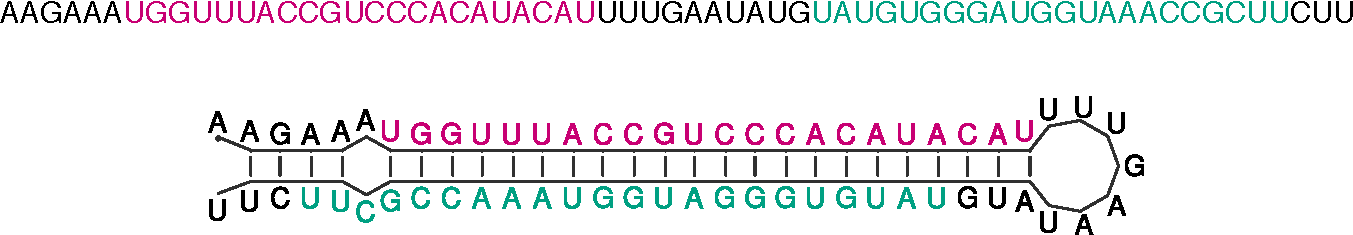
\includegraphics[width=\textwidth]{figures/hsa-mir-299_ss/hsa-mir-299_ss.pdf}
%nnodes = 75
\shorthandoff{<}
\shorthandoff{>}
\tikzsetnextfilename{figures/hsa-mir-299_ss/hsa-mir-299_ss}
\begin{tikzpicture}[scale=0.025,rotate=90,font=\relscale{0.9}\sffamily,
    every label/.style={label distance=0}]
\definecolor{rosa}{rgb}{0.78,0,0.45};
\definecolor{verde}{rgb}{0,0.63,0.51};
\definecolor{ro}{rgb}{0.78,0,0.45};
\definecolor{ve}{rgb}{0,0.63,0.51};
%\definecolor{}{rgb}{0,0,0};

\tikzstyle{lstyle}=[shorten >= 2,shorten <= 2];
  \foreach \q / \colr [count=\c] in {
 A/black, A/black, G/black, A/black, A/black, A/black, U/ro, G/ro,
 G/ro, U/ro, U/ro, U/ro, A/ro, C/ro, C/ro, G/ro, U/ro, C/ro, C/ro,
 C/ro, A/ro, C/ro, A/ro, U/ro, A/ro, C/ro, A/ro, U/ro, U/black,
 U/black, U/black, G/black, A/black, A/black, U/black, A/black,
 U/black, G/black, U/ve, A/ve, U/ve, G/ve, U/ve, G/ve, G/ve, G/ve,
 A/ve, U/ve, G/ve, G/ve, U/ve, A/ve, A/ve, A/ve, C/ve, C/ve, G/ve,
 C/ve, U/ve, U/ve, C/black, U/black, U/black} {
    \pgfmathsetmacro\cpos{ 260 - \c * 10 };
    \node[anchor=center,color={\colr}] (ns\c)
    at (200,\cpos) {\q};
  }

  %%%%%%%%%%%%%%%%%%%%%%%%%%%%%%%%%%%%%%%%%%%%%%%%%%%%%%%%%%%%%%%%%%%%


\coordinate[label={[xshift=0,yshift=0]below:A}] (1) at (92.5000,172.2035);
\fill[] (1) circle (2.2);
\coordinate[label={[xshift=0,yshift=0]below:A}] (2) at (92.5000,157.2035);
\fill[] (2) circle (1.1);
\coordinate[label={[xshift=0,yshift=0]below:G}] (3) at (92.5000,142.2035);
\fill[] (3) circle (1.1);
\coordinate[label={[xshift=0,yshift=0]below:A}] (4) at (92.5000,127.2035);
\fill[] (4) circle (1.1);
\coordinate[label={[xshift=0,yshift=0]below:A}] (5) at (92.5000,112.2035);
\fill[] (5) circle (1.1);
\coordinate[label={[xshift=0,yshift=0]below:A}] (6) at (85.6761,100.0000);
\fill[] (6) circle (1.1);
\coordinate[label={[xshift=0,yshift=0,rosa]below:U}] (7) at (92.5000,87.7965);
\fill[] (7) circle (1.1);
\coordinate[label={[xshift=0,yshift=0,rosa]below:G}] (8) at (92.5000,72.7965);
\fill[] (8) circle (1.1);
\coordinate[label={[xshift=0,yshift=0,rosa]below:G}] (9) at (92.5000,57.7965);
\fill[] (9) circle (1.1);
\coordinate[label={[xshift=0,yshift=0,rosa]below:U}] (10) at (92.5000,42.7965);
\fill[] (10) circle (1.1);
\coordinate[label={[xshift=0,yshift=0,rosa]below:U}] (11) at (92.5000,27.7965);
\fill[] (11) circle (1.1);
\coordinate[label={[xshift=0,yshift=0,rosa]below:U}] (12) at (92.5000,12.7965);
\fill[] (12) circle (1.1);
\coordinate[label={[xshift=0,yshift=0,rosa]below:A}] (13) at (92.5000,-2.2035);
\fill[] (13) circle (1.1);
\coordinate[label={[xshift=0,yshift=0,rosa]below:C}] (14) at (92.5000,-17.2035);
\fill[] (14) circle (1.1);
\coordinate[label={[xshift=0,yshift=0,rosa]below:C}] (15) at (92.5000,-32.2035);
\fill[] (15) circle (1.1);
\coordinate[label={[xshift=0,yshift=0,rosa]below:G}] (16) at (92.5000,-47.2035);
\fill[] (16) circle (1.1);
\coordinate[label={[xshift=0,yshift=0,rosa]below:U}] (17) at (92.5000,-62.2035);
\fill[] (17) circle (1.1);
\coordinate[label={[xshift=0,yshift=0,rosa]below:C}] (18) at (92.5000,-77.2035);
\fill[] (18) circle (1.1);
\coordinate[label={[xshift=0,yshift=0,rosa]below:C}] (19) at (92.5000,-92.2035);
\fill[] (19) circle (1.1);
\coordinate[label={[xshift=0,yshift=0,rosa]below:C}] (20) at (92.5000,-107.2035);
\fill[] (20) circle (1.1);
\coordinate[label={[xshift=0,yshift=0,rosa]below:A}] (21) at (92.5000,-122.2035);
\fill[] (21) circle (1.1);
\coordinate[label={[xshift=0,yshift=0,rosa]below:C}] (22) at (92.5000,-137.2035);
\fill[] (22) circle (1.1);
\coordinate[label={[xshift=0,yshift=0,rosa]below:A}] (23) at (92.5000,-152.2035);
\fill[] (23) circle (1.1);
\coordinate[label={[xshift=0,yshift=0,rosa]below:U}] (24) at (92.5000,-167.2035);
\fill[] (24) circle (1.1);
\coordinate[label={[xshift=0,yshift=0,rosa]below:A}] (25) at (92.5000,-182.2035);
\fill[] (25) circle (1.1);
\coordinate[label={[xshift=0,yshift=0,rosa]below:C}] (26) at (92.5000,-197.2035);
\fill[] (26) circle (1.1);
\coordinate[label={[xshift=0,yshift=0,rosa]below:A}] (27) at (92.5000,-212.2035);
\fill[] (27) circle (1.1);
\coordinate[label={[xshift=0,yshift=0,rosa]below:U}] (28) at (92.5000,-227.2035);
\fill[] (28) circle (1.1);
\coordinate[label={[xshift=0,yshift=0]below:U}] (29) at (80.4054,-237.1159);
\fill[] (29) circle (1.1);
\coordinate[label={[xshift=0,yshift=0]below:U}] (30) at (77.5628,-252.4929);
\fill[] (30) circle (1.1);
\coordinate[label={[xshift=0,yshift=0]below:U}] (31) at (85.3143,-266.0741);
\fill[] (31) circle (1.1);
\coordinate[label={[xshift=0,yshift=0]right:G}] (32) at (100.0000,-271.4467);
\fill[] (32) circle (1.1);
\coordinate[label={[xshift=0,yshift=0]above:A}] (33) at (114.6857,-266.0741);
\fill[] (33) circle (1.1);
\coordinate[label={[xshift=0,yshift=0]above:A}] (34) at (122.4372,-252.4929);
\fill[] (34) circle (1.1);
\coordinate[label={[xshift=0,yshift=0]above:U}] (35) at (119.5946,-237.1159);
\fill[] (35) circle (1.1);
\coordinate[label={[xshift=0,yshift=0]above:A}] (36) at (107.5000,-227.2035);
\fill[] (36) circle (1.1);
\coordinate[label={[xshift=0,yshift=0]above:U}] (37) at (107.5000,-212.2035);
\fill[] (37) circle (1.1);
\coordinate[label={[xshift=0,yshift=0]above:G}] (38) at (107.5000,-197.2035);
\fill[] (38) circle (1.1);
\coordinate[label={[xshift=0,yshift=0,verde]above:U}] (39) at (107.5000,-182.2035);
\fill[] (39) circle (1.1);
\coordinate[label={[xshift=0,yshift=0,verde]above:A}] (40) at (107.5000,-167.2035);
\fill[] (40) circle (1.1);
\coordinate[label={[xshift=0,yshift=0,verde]above:U}] (41) at (107.5000,-152.2035);
\fill[] (41) circle (1.1);
\coordinate[label={[xshift=0,yshift=0,verde]above:G}] (42) at (107.5000,-137.2035);
\fill[] (42) circle (1.1);
\coordinate[label={[xshift=0,yshift=0,verde]above:U}] (43) at (107.5000,-122.2035);
\fill[] (43) circle (1.1);
\coordinate[label={[xshift=0,yshift=0,verde]above:G}] (44) at (107.5000,-107.2035);
\fill[] (44) circle (1.1);
\coordinate[label={[xshift=0,yshift=0,verde]above:G}] (45) at (107.5000,-92.2035);
\fill[] (45) circle (1.1);
\coordinate[label={[xshift=0,yshift=0,verde]above:G}] (46) at (107.5000,-77.2035);
\fill[] (46) circle (1.1);
\coordinate[label={[xshift=0,yshift=0,verde]above:A}] (47) at (107.5000,-62.2035);
\fill[] (47) circle (1.1);
\coordinate[label={[xshift=0,yshift=0,verde]above:U}] (48) at (107.5000,-47.2035);
\fill[] (48) circle (1.1);
\coordinate[label={[xshift=0,yshift=0,verde]above:G}] (49) at (107.5000,-32.2035);
\fill[] (49) circle (1.1);
\coordinate[label={[xshift=0,yshift=0,verde]above:G}] (50) at (107.5000,-17.2035);
\fill[] (50) circle (1.1);
\coordinate[label={[xshift=0,yshift=0,verde]above:U}] (51) at (107.5000,-2.2035);
\fill[] (51) circle (1.1);
\coordinate[label={[xshift=0,yshift=0,verde]above:A}] (52) at (107.5000,12.7965);
\fill[] (52) circle (1.1);
\coordinate[label={[xshift=0,yshift=0,verde]above:A}] (53) at (107.5000,27.7965);
\fill[] (53) circle (1.1);
\coordinate[label={[xshift=0,yshift=0,verde]above:A}] (54) at (107.5000,42.7965);
\fill[] (54) circle (1.1);
\coordinate[label={[xshift=0,yshift=0,verde]above:C}] (55) at (107.5000,57.7965);
\fill[] (55) circle (1.1);
\coordinate[label={[xshift=0,yshift=0,verde]above:C}] (56) at (107.5000,72.7965);
\fill[] (56) circle (1.1);
\coordinate[label={[xshift=0,yshift=0,verde]above:G}] (57) at (107.5000,87.7965);
\fill[] (57) circle (1.1);
\coordinate[label={[xshift=0,yshift=0,verde]above:C}] (58) at (114.3239,100.0000);
\fill[] (58) circle (1.1);
\coordinate[label={[xshift=0,yshift=0,verde]above:U}] (59) at (107.5000,112.2035);
\fill[] (59) circle (1.1);
\coordinate[label={[xshift=0,yshift=0,verde]above:U}] (60) at (107.5000,127.2035);
\fill[] (60) circle (1.1);
\coordinate[label={[xshift=0,yshift=0]above:C}] (61) at (107.5000,142.2035);
\fill[] (61) circle (1.1);
\coordinate[label={[xshift=0,yshift=0]above:U}] (62) at (107.5000,157.2035);
\fill[] (62) circle (1.1);
\coordinate[label={[xshift=0,yshift=0]above:U}] (63) at (107.5000,172.2035);
\fill[] (63) circle (1.1);
\draw[lstyle] (1) -- (2);
\draw[lstyle] (2) -- (3);
\draw[lstyle] (3) -- (4);
\draw[lstyle] (4) -- (5);
\draw[lstyle] (5) -- (6);
\draw[lstyle] (6) -- (7);
\draw[lstyle] (7) -- (8);
\draw[lstyle] (8) -- (9);
\draw[lstyle] (9) -- (10);
\draw[lstyle] (10) -- (11);
\draw[lstyle] (11) -- (12);
\draw[lstyle] (12) -- (13);
\draw[lstyle] (13) -- (14);
\draw[lstyle] (14) -- (15);
\draw[lstyle] (15) -- (16);
\draw[lstyle] (16) -- (17);
\draw[lstyle] (17) -- (18);
\draw[lstyle] (18) -- (19);
\draw[lstyle] (19) -- (20);
\draw[lstyle] (20) -- (21);
\draw[lstyle] (21) -- (22);
\draw[lstyle] (22) -- (23);
\draw[lstyle] (23) -- (24);
\draw[lstyle] (24) -- (25);
\draw[lstyle] (25) -- (26);
\draw[lstyle] (26) -- (27);
\draw[lstyle] (27) -- (28);
\draw[lstyle] (28) -- (29);
\draw[lstyle] (29) -- (30);
\draw[lstyle] (30) -- (31);
\draw[lstyle] (31) -- (32);
\draw[lstyle] (32) -- (33);
\draw[lstyle] (33) -- (34);
\draw[lstyle] (34) -- (35);
\draw[lstyle] (35) -- (36);
\draw[lstyle] (36) -- (37);
\draw[lstyle] (37) -- (38);
\draw[lstyle] (38) -- (39);
\draw[lstyle] (39) -- (40);
\draw[lstyle] (40) -- (41);
\draw[lstyle] (41) -- (42);
\draw[lstyle] (42) -- (43);
\draw[lstyle] (43) -- (44);
\draw[lstyle] (44) -- (45);
\draw[lstyle] (45) -- (46);
\draw[lstyle] (46) -- (47);
\draw[lstyle] (47) -- (48);
\draw[lstyle] (48) -- (49);
\draw[lstyle] (49) -- (50);
\draw[lstyle] (50) -- (51);
\draw[lstyle] (51) -- (52);
\draw[lstyle] (52) -- (53);
\draw[lstyle] (53) -- (54);
\draw[lstyle] (54) -- (55);
\draw[lstyle] (55) -- (56);
\draw[lstyle] (56) -- (57);
\draw[lstyle] (57) -- (58);
\draw[lstyle] (58) -- (59);
\draw[lstyle] (59) -- (60);
\draw[lstyle] (60) -- (61);
\draw[lstyle] (61) -- (62);
\draw[lstyle] (62) -- (63);
\draw[lstyle] (1) -- (63);
\draw[lstyle] (2) -- (62);
\draw[lstyle] (3) -- (61);
\draw[lstyle] (4) -- (60);
\draw[lstyle] (5) -- (59);
\draw[lstyle] (7) -- (57);
\draw[lstyle] (8) -- (56);
\draw[lstyle] (9) -- (55);
\draw[lstyle] (10) -- (54);
\draw[lstyle] (11) -- (53);
\draw[lstyle] (12) -- (52);
\draw[lstyle] (13) -- (51);
\draw[lstyle] (14) -- (50);
\draw[lstyle] (15) -- (49);
\draw[lstyle] (16) -- (48);
\draw[lstyle] (17) -- (47);
\draw[lstyle] (18) -- (46);
\draw[lstyle] (19) -- (45);
\draw[lstyle] (20) -- (44);
\draw[lstyle] (21) -- (43);
\draw[lstyle] (22) -- (42);
\draw[lstyle] (23) -- (41);
\draw[lstyle] (24) -- (40);
\draw[lstyle] (25) -- (39);
\draw[lstyle] (26) -- (38);
\draw[lstyle] (27) -- (37);
\draw[lstyle] (28) -- (36);
\end{tikzpicture}
\shorthandon{<}
\shorthandon{>}


\caption{\captionStyle\protect\label{horquilla}
Secuencia (arriba) y estructura secundaria tipo horquilla (abajo) del
pre-miRNA de la especie humana \sbs{hsa-mir-299}.  Los fragmentos de
secuencia coloreados corresponden a los miRNAs \sbs{hsa-mir-299-5p}
(rosa) y \sbs{hsa-mir-299-3p} (verde).
}
\end{figure}
La forma clásica de identificación de nuevos \premirna{s} son las
pruebas experimentales de laboratorio.
Sin embargo, este tipo de pruebas sólo pueden identificar con
fiabilidad aquellos \premirna{s} abundantes dentro de la célula.
Las técnicas computacionales son una alternativa a las pruebas de
laboratorio que superan estas dificultades, ya que al extraer la
información directamente a partir del genoma de cada organismo,
permiten encontrar aquellos \premirna{s} que son específicos a
determinados tipos de tejidos o estadíos de desarrollo celular, y
aquellos escasamente expresados \cite{ding,sheng,xu}.

%
%
%
\section{Clasificación de \premirna{s}}
%
Los métodos de la Inteligencia Computacional utilizados para
clasificación de \premirna{s} son técnicas de \e{aprendizaje
  supervisado}.
En general, estas técnicas permiten generar un \e{modelo} o
representación interna que caracteriza los \premirna{s}, extrayendo
información a partir de un conjunto de datos de ejemplo denominado
\e{conjunto de entrenamiento}.
Se dice que el modelo generado posee capacidad de \e{generalización},
ya que puede ser aplicado sobre nuevos ejemplos que no le han sido
presentados con anterioridad.
El modelo funciona como un \e{clasificador}, discriminando los
ejemplos en diferentes \e{clases}.
Se considera el caso de la clasificación binaria, asociando una clase
``positiva'' a los \premirna{s} reales, y una clase ``negativa'' a los
ejemplos que son de otro tipo.
En el presente trabajo se generan clasificadores binarios de
secuencias de \premirna{s} utilizando técnicas de aprendizaje
supervisado mediante el \e{perceptrón multicapa} \cite{mlp1,mlp2} y la
\e{máquina de vectores de soporte} \cite{svm}.

El perceptrón multicapa (\e{MLP}, del inglés \eng{Multi-Layer
  Perceptron}) es un tipo de red neuronal artificial con propagación
hacia adelante, en la que se disponen nodos computadores (neuronas)
organizados en \e{capas}.
La salida de cada neurona se determina al aplicar una \e{función de
  activación}, de tipo sigmoidea, a una suma ponderada de las salidas
en la capa anterior.
Durante el entrenamiento del perceptrón multicapa, se ajustan
progresivamente los pesos (ponderaciones) de cada neurona mediante un
algoritmo de aprendizaje basado en la \e{propagación hacia atrás} del
error de clasificación, hasta satisfacer un criterio de corte
\cite{jain}.

La máquina de vectores de soporte (\e{SVM}, de su nombre en inglés
\eng{Support Vector Machine}) es un algoritmo de clasificación que se
basa en transformar, mediante una función llamada \e{núcleo}, el
espacio $N$-dimensional de los datos de entrada en otro espacio de
dimensión $M: M\gg N$, donde se espera que los datos sean linealmente
separables mediante un hiperplano.
El entrenamiento consiste en encontrar resolver un problema de
optimización que determina un hiperplano de separación óptimo para los
datos presentados, maximizando la distancia a los ejemplos más
cercanos en el espacio transformado \cite{bottou}.

%
%
%
\section{Motivación}
%
El debate acerca del número e identidad de los miRNAs presentes en
diferentes genomas es una cuestión abierta.
A modo de ejemplo, para el caso del genoma humano se había estimado
inicialmente que se encontrarían unos pocos cientos de genes miRNA;
posteriormente este número ha sido revisado a unos 1000
\cite{sewer,chang}.
Actualmente, se encuentra que el número de miRNAs descubiertos en
humanos duplica esta cifra \cite{gomes}.
Asimismo, este número podría ser mucho mayor si se considera que
existen miRNAs de evolución más reciente, específicos a la especie
humana \cite{sewer}.

Este proyecto se origina en el Centro de Investigación en Señales, 
Sistemas e Inteligencia Computacional \e{sinc(i)} ante la necesidad de
contar con un nuevo modelo para la clasificación de \premirna{s} que
complemente a los desarrollos existentes en la disciplina y que sea
de fácil utilización por parte del usuario no experto en Inteligencia
Computacional.

%Con este desarrollo se pretende que los especialistas \hl{especificar}
%cuenten con una herramienta sencilla para la aplicación de técnicas
%avanzadas de clasificación, e integrada a su flujo de trabajo
%habitual.

%
%
%
\section{Objetivos}
%
El objetivo general del proyecto es desarrollar un método de
clasificación de \premirna{s} mediante clasificadores MLP y SVM,
abarcando desde el procesamiento de los datos de entrada hasta la
obtención de las predicciones de clase para nuevos ejemplos.

Adicionalmente, se pretende que el método desarrollado tenga un alto
grado de automatización de los aspectos que no sean especialidad del
usuario final, brindando facilidad de uso con buenos resultados de
clasificación.
%
%
\subsection{Objetivos específicos}
%
\begin{itemize}
\item Recopilar bases de datos de ejemplos de clase positiva y
  negativa.
\item Diseñar un método de extracción de \caract{s} sobre estos datos
  replicando técnicas presentes en la bibliografía.
\item Codificar los métodos de entrenamiento y clasificación.
\item Mediante pruebas sobre las bases de datos recopiladas determinar
  parámetros/configuraciones óptimas de clasificación.
\item Codificar métodos de selección automática de \hparam{s}
  \hl{esto no estaba en el anteproyecto}.
\item Codificar y documentar una interfaz de línea de comandos, y una
  interfaz web orientada al usuario final.
\item Efectuar pruebas del método final documentando los resultados
  obtenidos.
\end{itemize}
%

%
%
\subsection{Objetivos específicos}
%
\begin{itemize}
\item Recopilar bases de datos con ejemplos de clase positiva y
  negativa.
\item Diseñar y codificar un método de extracción de \caract{s} sobre
  estos datos replicando técnicas presentes en la bibliografía.
\item Diseñar y codificar métodos para la generación del modelo del
  clasificador, determinando parámetros adecuados para el
  entrenamiento. 
\item Diseñar y codificar los métodos necesarios para la clasificación
  aplicando el modelo generado sobre nuevos datos.
\item Codificar y documentar una interfaz de línea de comandos, y una
  interfaz web orientada al usuario final.
\item Efectuar pruebas del método final con los datos disponibles y
  documentar los resultados obtenidos.
\end{itemize}
%

%
%
%
\section{Alcances}
%
\begin{itemize}
\item
  El trabajo se centra en la etapa de generación del modelo del
  clasificador y su aplicación como clasificador, aplicando tanto
  Máquinas de Vectores de Soporte (SVMs) como Perceptrones Multicapa
  (MLPs).
\item
  Se trabajará durante el desarrollo exclusivamente con datos de
  prueba disponibles en línea, cuya pertenencia de clase sea conocida
  y validada experimentalmente.
\item
  No se pretende innovar en el campo de la extracción de \caract{s},
  por lo que en el presente trabajo se aplicarán técnicas propuestas
  por otros autores.
\item
  El objetivo del método a desarrollar es la identificación de
  \premirna{s}, quedando fuera del alcance de este proyecto la
  identificación de los miRNA maduros contenidos dentro de los mismos.
\item
  El proyecto no persigue el desarrollo de un producto o servicio
  comercial.
\end{itemize}
%

%
%
%
%
\chapter{Fundamentos teóricos}
%
El propósito principal del presente proyecto es generar una aplicación
de técnicas de la Inteligencia Computacional (IC) sobre un tipo de dato
específico, las cadenas de \premirna{s}.
La Inteligencia Computacional es la disciplina que estudia la
aplicación de técnicas y metodologías inspiradas en la naturaleza para
resolver problemas complejos.
En general, las técnicas de IC presentan cualidades típicas del
razonamiento humano, ``generalizando'' el conocimiento inexacto o 
incompleto, y son capaces de tomar decisiones en forma adaptativa.

En el presente Capítulo se presenta una introducción teórica a los
conceptos fundamentales de la IC en general, en particular del área del
\e{aprendizaje supervisado}.
Más adelante, se describen las técnicas específicas aplicadas en el
presente trabajo: el perceptrón multicapa y la máquina de vectores de
soporte.

%
%
%
\section{La clasificación como forma de aprendizaje supervisado}
%
En el contexto de la Inteligencia Computacional, la clasificación es
un tipo de \e{aprendizaje supervisado} cuyo objetivo es
{inferir} una función que relaciona \e{datos de entrada} con las
respectivas \e{salidas deseadas}, a partir de una serie de ejemplos que
conforman el llamado \e{conjunto de entrenamiento}.
Un algoritmo que implementa la clasificación se conoce como un
\e{clasificador}.
La función que transforma los datos de entrada a una categoría
(clase) se llama \e{modelo} (o {hipótesis}).

Un clasificador es un tipo de \e{máquina de aprendizaje}, y consiste
en un algoritmo que analiza los datos del conjunto de entrenamiento
y produce una función de correspondencia (el modelo) que puede ser
usada para relacionar nuevos ejemplos (datos de entrada) a una clase
(valor de salida).
De este modo, el clasificador es capaz de replicar el comportamiento
del sistema o proceso que pretende modelar, y se dice que el modelo
obtenido es capaz de \e{generalizar} a partir de los datos de
entrenamiento.

A continuación, se presentan definiciones de los conceptos
relevantes del aprendizaje supervisado.
%{La discusión se basa en aquella presentada en \cite{glasmachers}.}

%
%
\subsection{Conceptos básicos del aprendizaje supervisado}
%
A continuación se presentan definiciones de los conceptos básicos
utilizados en el ámbito de la Inteligencia Computacional en relación
al aprendizaje automáico.

%
\subsubsection{Aprendizaje supervisado}
%
Sean $X$ e $Y$ espacios vectoriales, y sea $(\xx,\yy)\in{}X\times{}Y$
un \e{ejemplo} (representando a una observación) que relaciona una
entrada $\xx\in{}X$ con la salida correspondiente $\yy\in{}Y$.
%
Se asume que existe una distribución de probabilidades fija y
desconcida $\nu$ sobre el producto $X\times Y$, llamada
\e{distribución generadora} de los datos.
El aprendizaje supervisado
trata la extracción de propiedades de esta distribución a partir de un
número finito de variables aleatorias, denominadas \e{ejemplos}, que
conforman el conjunto de datos de entrenamiento
%
\begin{align}
  D = \left((\B{x}_1,\yy_1),\ldots,(\B{x}_\ell,\yy_\ell)\right) \in
  \mathcal{D}=\bigcup_{\ell=1}^\infty (X\times Y)^\ell,
\end{align}
%
que se considera como una muestra independiente e idénticamente
distribuida de $\nu$, esto es, $D\sim\nu$.

%
\subsubsection{Modelo}
%
En un problema típico de aprendizaje supervisado, se trata de
encontrar una función medible $h:X\rightarrow{}Y$ que {modela} las
propiedades más importantes de la distribución $\nu$. Esta función
se denomina \e{modelo} o \e{hipótesis}, y representa el
fenómeno real que da origen a los datos relacionando el espacio de
entrada $X$ con el de salida $Y$.

%
\subsubsection{Máquina de aprendizaje}
%
Sea $\C{H}=\{h:X\rightarrow Y\}$ el conjunto de todos los modelos
posibles.
Una máquina de aprendizaje es una transformación
%
\begin{align}
  A:\mathcal{D}\rightarrow\C{H}
  \label{eq:maqaprendizaje}
\end{align}
%
que relaciona un conjunto de datos a un modelo.
La máquina de aprendizaje $A$ no es necesariamente una transformación
en el sentido matemático, sino que en general se trata de un algoritmo
que efectúa el proceso denominado \e{entrenamiento}.

%
\subsubsection{Clasificador}
%
Se dice que se está ante un problema de \e{clasificación} cuando el
espacio de las salidas $Y$ es un conjunto discreto y finito, donde
cada valor posible de $Y$ se corresponde con una categoría o
\emph{clase}.
El caso más básico e importante es el de la
\e{clasificación binaria}, en la que se consideran sólo dos valores en
$Y$, comúnmente $+1$ (``positivo'') y $-1$ (``negativo'').

Un \e{clasificador} es, entonces, el caso especial de una máquina de
aprendizaje cuando el espacio de salida $Y$ es discreto y finito.
Naturalmente, siempre que se hable de máquinas de aprendizaje se
incluyen los clasificadores dentro de esta denominación.

%
\subsubsection{Función de pérdida}
%
Para un ejemplo $(\xx,\yy)\in{}X\times{}Y$, la función de pérdida mide
la cantidad de error del modelo $\hat{\yy}=h(\xx)$ mediante la
transformación $L(\xx,\yy,\hat{\yy})$.
Si la predicción resultante
del modelo $\hat{\yy}$ es correcta, el error es nulo.
En la práctica,
la mayoría de las funciones de pérdida no dependen de la entrada
$\xx$, sino sólo de la predicción $\hat{\yy}$ y la clase $\yy$.
Algunas de las funciones de pérdida más comunes son:
%
\begin{align}
  \T{Pérdida 0-1:} \tab\tabs
    L(\yy,\hat{\yy})=\begin{cases}0,\quad{}\yy=\hat{\yy}\\
      1,\quad\T{en otro caso}\end{cases} \\
  \T{Pérdida ``bisagra'':} \tab\tabs
    L(\yy,\hat{\yy})=\max\{0,\yy-\hat{\yy}\}\\
  \T{Error absoluto:} \tab\tabs
    L(\yy,\hat{\yy})=|\yy-\hat{\yy}|\\
  \T{Error cuadrático:} \tab\tabs
    L(\yy,\hat{\yy})=(\yy-\hat{\yy})^2.
\end{align}
%

%
\subsubsection{Error de generalización}
%
El error de generalización
$\mathcal{R}_\nu:\C{H}\rightarrow\RR^{\geq0}$ es el error esperado de
un modelo $h$ al clasificar un ``nuevo'' ejemplo independiente
del conjunto $D$, y se define a partir de la función de pérdida $L$ según
%
\begin{align}
  \mathcal{R}_\nu=\mathds{E}_\nu\left[L(\xx,\yy,h(\xx))\right]
  =\int_{X\times Y} L(\xx,\yy,h(\xx))\, d\nu(\xx,\yy).
\end{align}
%
Para poder calcular el error de generalización se requiere conocer la
distribución generadora de datos $\nu$.
Sin embargo, toda la información disponible de $\nu$ es la muestra $D$,
de probabilidad desconocida.
Entonces, la aplicación del concepto de error de generalización es
teórica, y en la práctica se utilizarán otras medidas de error para
aproximarlo.

%% El cálculo de este error requiere conocer la distribución generadora
%% de datos $\nu$.
%% Sin embargo, toda la información que se tiene de $\nu$
%% es la realización $D$, para la cual no se conoce su probabilidad.
%% Por ello, la aplicación del concepto de error de generalización es
%% teórica, y se utilizan en la práctica medidas que lo aproximan.

%
%
\subsection{Entrenamiento}
%
El entrenamiento es el proceso de construir un modelo $h(\xx)$ a
partir de los datos del conjunto de entrenamiento
$D=\left((\xx_1,\yy_1),\ldots,(\xx_\ell,\yy_\ell)\right)$.
Este conjunto es una muestra (de probabilidad desconocida) de la
distribución generadora de datos $\nu$, y define una distribución
\e{empírica}
%
\begin{align}
  \hat{\nu}=\frac{1}{\ell}\sum_{i=1}^{\ell}\delta_{(\xx_i,\yy_i)}(\xx,\yy)
\end{align}
%
donde $\delta_{(\xx,\yy)}$ denota el delta de Dirac en
$(\xx,\yy)\in{}X\times{}Y$.
%
\subsubsection{Error de entrenamiento}
%
La distribución empírica $\hat{\nu}$ conduce a la definición del
\e{error de entrenamiento} como el error del modelo $h$ sobre los
datos de entrenamiento en $D$:
%
\begin{align}
  \hat{\C{R}}_D(h)=E_\T{entrenamiento}=\R{E}_{\hat{\nu}}[L(\xx,\yy,h(\xx))]
  =\frac{1}{\ell}\sum_{i=1}^\ell L(\xx_i, \yy_i, h(\xx_i)),
\end{align}
%
en donde $L$ es una función de pérdida.
%

%
Una forma de entrenamiento básica de la máquina de aprendizaje consiste en
seleccionar el modelo con el mínimo error de entrenamiento
%
\begin{align}
  \hat{h}:=\arg \min \left\{ \hat{\C{R}}_D(h)\middle|h \in H\right\}.
\end{align}
%
Este procedimiento se conoce también como la minimización del riesgo
empírico sobre el conjunto de entrenamiento.

%
\subsubsection{Parámetros del modelo}
%
Considerando al modelo $\hat{\yy}=h(\xx)$ como un caso específico
de una familia de funciones más general $\hat{y}=H(\xx,\B{p})$, se dice
que $\B{p}$ es un vector de \e{parámetros} que determinan la respuesta
de $H$ ante una entrada $\xx$.
Desde este punto de vista, puede entenderse el {entrenamiento} como el
proceso de determinar los parámetros óptimos $\B{p}$ que definen el modelo
$h$, minimizando el error promedio de $H$ sobre el conjunto de datos $D$.

%
\subsubsection{Hiperparámetros}
%
Se denomina \e{hiperparámetros} a aquellos parámetros que regulan el 
proceso de entrenamiento, que sin formar parte del modelo influyen en
la generación del mismo.
En general, los \hparam{s} determinan el comportamiento de ``alto nivel''
del algoritmo de entrenamiento, tal como la cantidad de ajuste aplicado al
modelo en cada iteración, el grado de tolerancia a los errores, o la
complejidad de la solución.

Al actuar como reguladores del proceso de entrenamiento, los \hparam{s}
deben ser establecidos antes de comenzar el mismo.
En general, la selección de los hiperparámetros se efectúa mediante prueba
y error sobre modelos desechables, ya sea en forma manual o mediante un
algoritmo automático.
Para ciertos tipos específicos de máquina de aprendizaje, existen técnicas
automáticas que configuran los \hparam{s} de manera eficiente.

%
\subsubsection{Error de entrenamiento}
%
El conjunto de entrenamiento $D$ es una muestra (de probabilidad
desconocida) de la distribución generadora de los datos $\nu$.
Esta muestra determina una distribución \e{empírica}
%
\begin{align}
  \hat{\nu}=\frac{1}{\ell}\sum_{i=1}^{\ell}\delta_{(\xx_i,\yy_i)}(\xx,\yy),
\end{align}
%
en donde $\delta_{(\xx,\yy)}$ es la delta de Dirac centrada en el
punto $(\xx,\yy)$.
La distribución $\hat{\nu}$ conduce a la definición del
\e{error de entrenamiento} como el error del modelo $h$ sobre los
datos de entrenamiento en $D$:
%
\begin{align}
  \hat{\C{R}}_D(h)=E_\T{entrenamiento}=\R{E}_{\hat{\nu}}[L(\xx,\yy,h(\xx))]
  =\frac{1}{\ell}\sum_{i=1}^\ell L(\xx_i, \yy_i, h(\xx_i)),
\end{align}
%
en donde $L$ es una función de pérdida.
La forma de entrenamiento más básica e importante de una máquina
de aprendizaje consiste en seleccionar el modelo que minimiza el
error de entrenamiento
%
\begin{align}
  \hat{h}:=\arg \min \left\{ \hat{\C{R}}_D(h)\middle|h \in H\right\}.
\end{align}
%
Este procedimiento se conoce también como la minimización del riesgo
empírico sobre el conjunto de entrenamiento.

%
\subsubsection{Sobreajuste}
%
El objetivo teórico del entrenamiento debe ser
encontrar el modelo con mayor capacidad de generalización, que
describa con el menor error posible la distribución $\nu$.
Sin embargo, toda la información disponible es el conjunto $D$, que no
es más que una muestra de probabilidad desconocida del fenómeno
descripto por $\nu$.
Esta distinción entre error de entrenamiento y
error de generalización debe ser tenida en cuenta al efectuar el
entrenamiento, para evitar que el modelo \e{sobreajuste} los datos.

Se dice que un modelo presenta \e{sobreajuste} cuando éste describe
el conjunto de entrenamiento $D$ en lugar de la relación
subyacente $\nu$ entre las variables de entrada y de salida.
Intuitivamente, el modelo sobreajustado
\e{memoriza ejemplos} del conjunto de entrenamiento en lugar de
\e{describir las propiedades} de la distribución $\nu$.
El problema del sobreajuste existe debido a que la máquina de
aprendizaje no recibe información acerca de la \e{probabilidad}
de cada ejemplo observado, ignorando el ruido y los efectos
aleatorios en el conjunto de datos de entrenamiento.

%
\subsubsection{Sesgo y varianza}
%
Los conceptos de sesgo y varianza brindan un marco de análisis para
los algoritmos de aprendizaje automático.
Desde esta perspectiva, se
identifican tres fuentes de error de generalización del modelo: el
sesgo, la varianza, y el error intrínseco, irreducible, debido a la
incertidumbre inherente a los datos.
%
\begin{itemize}
\item El sesgo hace referencia al error cometido por el modelo sobre
  el conjunto de entrenamiento. Un bajo sesgo significa que el modelo
  ``ajusta bien'' al conjunto de entrenamiento.
\item La varianza se relaciona con la complejidad del modelo. Cuando
  el modelo se torna más complejo, se vuelve susceptible a pequeñas
  variaciones en los datos de entrada, perdiendo generalidad en la
  salida.
\end{itemize}
%
El objetivo del entrenamiento es ajustar suficientemente el modelo
(bajar el sesgo) cuidando de no aumentar demasiado su complejidad
(aumentando la varianza).  Este problema se denomina frecuentemente
``el dilema sesgo--varianza''.

%% Un modelo subajustado tendrá un alto sesgo, mientras
%% que un modelo sobreajustado tendrá una alta varianza.

%% Las medidas de sesgo y varianza son útiles para los modeladores en
%% tanto que ayudan a regular la complejidad del modelo final.

%% Estas medidas se relacionan con la capacidad de ajuste y
%% generalización de un modelo.

%% Cuando se logra un gran ajuste, la diferencia entre los datos reales y
%% la estimación del modelo es pequeña, en este caso el sesgo también es
%% pequeño, pero estos buenos resultados de ajuste, van de la mano con
%% el aumento en la complejidad del modelo, cuando se aumenta la
%% complejidad del modelo este se vuelve sensible a pequeñas variaciones
%% en los datos de entrada, fluctuando en función de estos, es así cuan-
%% do la varianza aumenta.

%% Esta claro que en Aprendizaje de Maquina se busca crear modelos que
%% ofrezcan dos características esenciales: ajuste a los datos y
%% generalización.

%% Esto acentúa la necesidad de encontrar un balance entre sesgo y
%% varianza, o visto de otra forma, entre error y complejidad, a
%% continuación se describen algunos conceptos importantes referentes al
%% tema.

%% %
%% \subsubsection{El <<dilema sesgo--varianza>>}
%% %
%% El \e{dilema sesgo--varianza} hace referencia al problema de minimizar
%% simultáneamente dos fuentes de error que impiden que la máquina de
%% aprenzizaje generalizar más allá del conjunto de entrenamiento:
%% %
%% \begin{itemize}
%% \item El sesgo es el error producido por supuestos erróneos en el
%%   algoritmo de aprendizaje.  Un sesgo elevado deriva en el algoritmo
%%   siendo incapaz de identificar las relaciones importantes entre las
%%   entradas y las salidas (subajuste).
%% \item La varianza es el error producido por la sensibilidad a pequeñas
%%   fluctuaciones en el conjunto de entrenamiento. Una alta varianza
%%   puede provocar sobreajuste.
%% \end{itemize}
%% %

%% The bias–variance decomposition is a way of analyzing a learning
%% algorithm's expected generalization error with respect to a particular
%% problem as a sum of three terms, the bias, variance, and a quantity
%% called the irreducible error, resulting from noise in the problem
%% itself.

%% This tradeoff applies to all forms of supervised learning:
%% classification, regression (function fitting),[1][2] and structured
%% output learning. It has also been invoked to explain the effectiveness
%% of heuristics in human learning.

%
%
\subsection{Estimación del error de generalización}
%
Un buen algoritmo de entrenamiento debe ser capaz de minimizar el
error de generalización del modelo tanto como sea posible.
Dado que el mismo resulta imposible de calcular sin conocer la
distribución generadora de los datos $\nu$, se recurre a otras
medidas para estimarlo.

%
\subsubsection{Error de prueba}
%
Dado un \e{conjunto de prueba}
$\,T=((\tilde{\xx}_1,\tilde{\yy}_1),\ldots,(\tilde{\xx}_N,\tilde{\yy}_N))$, el
\e{error de prueba} es la pérdida media del modelo sobre el conjunto $T$:
%
\begin{align}
  E_{\T{prueba}}=\frac{1}{N}\sum_{n=1}^N
  L(\tilde{\xx}_N,\tilde{\yy}_N,h(\tilde{\xx}_N)).
  \label{eq:error-prueba}
\end{align}
%
Este error de prueba es una estimación no sesgada del error de
generalización siempre que $T$ sea una muestra independiente e
idénticamente distribuida a $\nu$:
%
\begin{align}
  T\sim\nu^N.
  \label{eq:conj-prueba-sim-nu}
\end{align}
%
En la práctica, esta última condición no es más que un supuesto,
ya que no se dispone de información de la probabilidad
de la muestra $T$.

%
\subsubsection{Método de retención}
\label{retencion}
%
En un problema de aprendizaje típico, toda la información que se
conoce del fenómeno a modelar es una muestra $U\in\C{D}$ que contiene
todos los ejemplos conocidos.
El \e{método de retención} consiste en dividir el conjunto $U$ en dos
conjuntos disjuntos $D$ y $T$, que son usados respectivamente como
conjuntos de entrenamiento y de prueba.
La máquina de aprendizaje se entrena con el conjunto $D$, y el error
de generalización se estima midiendo el error del modelo sobre el
conjunto de prueba $T$.

En ocasiones, el conjunto de entrenamiento $D$ se subdivide siguiendo
el mismo procedimiento en conjuntos de \e{estimación} $E$ y
de \e{monitoreo} $M$.
Estos conjuntos son utilizados antes del entrenamiento para ajustar
los hiperparámetros del algoritmo de aprendizaje, generando modelos
de estimación que se evalúan con el conjunto de monitoreo $M$.
Una vez determinados los hiperparámetros, el modelo final se 
entrena con el conjunto de entrenamiento completo $D$.

%
\subsubsection{Validación cruzada de $k$ iteraciones}
\label{s2:crossval}
%
La validación cruzada es una técnica que permite estimar el error de
generalización probando (``validando'') el modelo sobre todos los
ejemplos del conjunto de entrenamiento.
En un procedimiento de \e{validación cruzada de $k$ iteraciones}
\cite{crossval}, el conjunto de entrenamiento $D$ se subdivide en $k$
conjuntos disjuntos $V_1,\ldots,V_k$ de tamaños similares, denominados
\e{particiones de validación}.
Para cada $i=1,\ldots,k$, se efectúa el entrenamiento sobre un
conjunto $D_i=D\setminus{}V_i$ que excluye a $V_i$, y se calcula la
tasa de error del modelo resultante sobre la partición $V_i$.
Una vez completado el proceso, se promedian las $k$ medidas de error
para obtener un estimador del error sobre el conjunto completo $D$.
Esta medida es un estimador más preciso del error de generalización
que la obtenida con el método de retención.
%% El costo computacional de la validación cruzada es $k$ veces
%% superior al del método de retención, y en general se justifica su
%% utilización

%
\subsubsection{Validación cruzada dejando uno fuera}
%
La \e{validación cruzada dejando uno fuera}
es el caso especial del procedimiento de validación cruzada 
cuando se establece el número de particiones $k$ igual al
número de elementos $\ell$ del conjunto de entrenamiento $D$.
Aplicando esta estrategia, el modelo obtenido en cada iteración
es muy similar a uno entrenado con el conjunto completo $D$.

La importancia de este procedimiento reside en el hecho que es el
mejor estimador del error de generalización de la máquina de aprendizaje.
En la práctica, no es muy utilizado debido a su elevado costo
computacional, ya que se requieren $\ell$ entrenamientos para su
cálculo.
Sin embargo, existen técnicas para el cálculo eficiente
para ciertas máquinas de aprendizaje específicas
\cite{chapelle,lee-keerthi}.

%
%
\subsection{Regularización}
%
Se dice que un modelo presenta sobreajuste cuando genera soluciones
relativamente complejas para problemas que en realidad tienden a ser
más simples.  Esto evoca un principio a menudo referido como la
\e{navaja de Ockam}: ``las entidades no deben multiplicarse más allá
de lo necesario'', afirmando que las explicaciones simples son más
plausibles y los modelos sencillos son más explicativos y más
confiables que los complicados.

La \e{regularización} consiste en forzar la simplicidad del modelo,
evitando el
sobreajuste del modelo generado por la máquina de aprendizaje. Existen
dos formas comunes para incorporar simplicidad en el modelo:
%
\begin{itemize}
\item Limitar el modelo a una subclase de funciones simples.
\item Añadir un término de penalización por complejidad al objetivo
  del error de entrenamiento.
\end{itemize}
%
Ambos procedimientos regularizan el proceso de aprendizaje, ya
que favorecen las hipótesis más simples.
El segundo enfoque requiere alguna forma de medir la ``complejidad'' del
modelo.

Cuando el entrenamiento de la máquina de aprendizaje es un proceso
gradual, una técnica alternativa de regularización consiste en
abortar el proceso de entrenamiento al momento que se detecta
que el error de generalización empieza a incrementarse.

Se debe notar que la regularización en general entra en conflicto con
la minimización del error de entrenamiento, y un modelo regularizado
cometerá más errores sobre el conjunto de entrenamiento que un modelo
no regularizado.  Sin embargo, se ha de esperar que el modelo
regularizado tenga mayor capacidad de generalización.

%%
%%
%\subsection{Selección automática de hiperparámetros}
%%
%La selección automática de hiperparámetros se efectúa antes del
%entrenamiento del modelo, mediante estrategias específicas para el
%tipo de clasificador y el tipo de hiperparámetro que se desea
%determinar.
%
%En general, esta selección se efectúa mediante técnicas de prueba y
%error, que entrenan un
%modelo preliminar sobre un conjunto de estimación y lo prueban contra
%un conjunto de validación, seleccionando los hiperparámetros que
%obtienen los mejores resultados según alguna métrica estadística.
%
%Para algunos clasificadores y tipos de hiperparámetros específicos,
%resulta posible la utilización de estrategias más ``informadas'' de
%selección de hiperparámetros, que aprovechan alguna propiedad teórica
%del tipo de modelo considerado y efectúan una búsqueda mediante
%descenso de gradiente minimizando una función derivable llamada
%``función objetivo''.

%
%
\subsection{Medidas de evaluación de un clasificador binario}
%
Los clasificadores binarios generan modelos cuya salida alterna
entre dos valores posibles, que se interpretan en forma genérica
como ``clase positiva'' y ``clase negativa''.
Para este tipo especialmente
importante de clasificadores, se utilizan una serie de métricas que
relacionan la pertenencia de clase de los datos con el
error de clasificación.

Dado un modelo $h$ de salida binaria, se definen las siguientes
medidas que caracterizan el resultado de clasificar un conjunto $T$:
%
\iflatexml\begin{itemize}\else\begin{itemize}[style=nextline]\fi
  \item\e{Verdaderos positivos ($\VP$)}: número de elementos de clase
    positiva correctamente clasificados como positivos.
  \item\e{Verdaderos negativos ($\VN$)}: número de elementos de clase
    negativa correctamente clasificados como negativos.
  \item\e{Falsos positivos ($\FP$)}: número de elementos de clase
    negativa erróneamente clasificados como positivos.
  \item\e{Falsos negativos ($\FN$)}: número de elementos de clase
    positiva erróneamente clasificados como negativos.
\end{itemize}
%
Estas cuatro medidas conforman la llamada \e{matriz de confusión}
característica del clasificador, y dependen en todos los casos del
número de elementos positivos y negativos presentes en el conjunto
$T$.

%
\subsubsection{Sensibilidad y especificidad}
%
A partir de los valores de la matriz de confusión se definen las
medidas de \e{sensibilidad ($\SE$)} y \e{especificidad ($\SP$)}:
%
\begin{align}
  \SE \tab = \frac{\VP}{\VP+\FN}, \tabs \SP \tab = \frac{\VN}{\VN+\FP}.
\end{align}
%
La sensibilidad, también llamada a veces \e{razón de veraderos
  positivos} (\e{TPR}), indica la \e{tasa de acierto} al clasificar
elementos de clase positiva, y la especificidad (también \e{razón de
  veraderos negativos}) representa la tasa de acierto al clasificar
ejemplos de clase negativa.
Ambas medidas son independientes del
número de elementos presentes en el conjunto de prueba, aunque no de
la proporción entre elementos positivos y negativos.

%% La importancia de las medidas de sensibilidad y especificidad es que
%% pueden utilizarse para elegir, por ejemplo, el clasificador con menor
%% cantidad de falsos negativos ($\SP=1$), una característica deseable en
%% aplicaciones tales como detectores de patógenos en bancos de sangre y
%% detectores de explosivos en aeropuertos.
%
\subsubsection{Media geométrica de la sensibilidad y  la especificidad}
%
En ocasiones, se requiere medir el funcionamiento de un clasificador a
partir de una única medida que caracterice la aptitud del clasificador
en general.
En estos casos, resulta común utilizar la media geométrica
entre la sensibilidad y la especificidad
%
\begin{align}
  \GM \tab = \sqrt{\SE\cdot\SP}.
\end{align}
%
%
\subsubsection{Otras medidas}
%
Otras medidas posibles para evaluar el comportamiento de un clasificador
binario son:
%
\begin{align}
    \T{Precisión} \tab\tabs \PR \tab=\frac{\VP}{\VP+\FP},\\
    \T{Exactitud} \tab\tabs \AC \tab=\frac{\VP+\VN}{\VP+\FP+\VN+\FN},\\
    \T{Valor-F}   \tab\tabs \T{\slshape F} \tab=\frac{\PR\cdot{}\SE}{\PR+\SE}, \\
    \iflatexml\T{Coef. corr. de Matthews}\else
    \parbox{4cm}{Coeficiente de correlación de Matthews}\fi \tab\tabs
    \T{\slshape MCC} \tab = \frac{\VP\cdot{}\VN-\FP\cdot\FN
    }{\sqrt{(\VP+\FP)(\VP+\FN)(\VN+\FP)(\VN+\FN)}}.
\end{align}
%
La precisión, por ejemplo, es la proporción aciertos de entre todos
los resultados positivos, y la exactitud es la proporción de
resultados correctos independientemente de la clase.

%
\subsubsection{Media geométrica de la sensibilidad y  la especificidad}
%
En ocasiones, se requiere medir el funcionamiento de un clasificador a
partir de una única medida que caracterice la aptitud del clasificador
en general.
En estos casos, resulta común utilizar la media geométrica
entre la sensibilidad y la especificidad
%
\begin{align}
  \GM \tab = \sqrt{\SE\cdot\SP}.
\end{align}
%

%
\subsubsection{Otras medidas}
%
Otras medidas posibles para evaluar el comportamiento de un clasificador
binario son:
%
\begin{align}
    \T{Precisión} \tab\tabs \PR \tab=\frac{\VP}{\VP+\FP},\\
    \T{Exactitud} \tab\tabs \AC \tab=\frac{\VP+\VN}{\VP+\FP+\VN+\FN},\\
    \T{Valor-F}   \tab\tabs \T{\slshape F} \tab=\frac{\PR\cdot{}\SE}{\PR+\SE}, \\
    \iflatexml\T{Coef. corr. de Matthews}\else
    \parbox{4cm}{Coeficiente de correlación de Matthews}\fi \tab\tabs
    \T{\slshape MCC} \tab = \frac{\VP\cdot{}\VN-\FP\cdot\FN
    }{\sqrt{(\VP+\FP)(\VP+\FN)(\VN+\FP)(\VN+\FN)}}.
\end{align}
%
La precisión, por ejemplo, es la proporción aciertos de entre todos
los resultados positivos, y la exactitud es la proporción de
resultados correctos independientemente de la clase.

%
%
%
\section{Perceptrón multicapa}
%
%% El perceptrón multicapa (\eng{MultiLayer Perceptron}, MLP)
%% \cite{mlp2,mlp1} es una red neuronal \feedforward{}
%% (\eng{feedforward}), consistente en una serie de {unidades} o
%% neuronas organizadas en \e{capas} y conectadas por ``enlaces''
%% denominados \e{pesos sinápticos}.  Las capas se diferencian en
%% una capa \e{de entrada}, una o más capas \e{ocultas} y una capa
%% \e{de salida}.

%% La capa de entrada contiene nodos sensores que ``leen'' un vector
%% de entrada externo, y lo transmiten a través de los enlaces sinápticos
%% a la primer capa oculta. Las capas ocultas reciben como entrada las
%% salidas de la capa anterior, determinan su valor de salida aplicando
%% una \e{función de activación} a la suma ponderada sus entradas, y
%% transmiten su valor de salida a la capa siguiente. Este proceso
%% continúa capa por capa hasta alcanzar la capa de salida.

%% Desde un punto de vista global, un vector arbitrario es propagado
%% \e{hacia adelante} a través de la red, para finalmente obtener un
%% vector de activación en la capa de salida.  La función generada por la
%% red, que transforma un vector de entrada en uno de salida, se
%% determina completamente por los pesos sinápticos de todos los enlaces
%% de la red.  En la \refer{fig:mlp} se puede observar una representación
%% esquemática de un perceptrón multicapa con 3 entradas, 4 neuronas en
%% la capa oculta y 2 valores de salida.

%% --------------

El perceptrón multicapa (\eng{MultiLayer Perceptron}, MLP)
\cite{mlp2,mlp1} es una máquina de aprendizaje basada en una red
neuronal artificial compuesta por {unidades} o neuronas
organizadas según una arquitectura de \e{capas}.

%% y conectadas por ``enlaces''
%% denominados \e{pesos sinápticos}
%% con una arquitectura organizada en capas.
%% Cada nodo se conecta mediante enlaces ponderados denominados
%% ``pesos sinápticos'' a todos los nodos en las capas adyacentes.

%% La primer capa, denominada capa de entrada, contiene nodos sensores
%% que ``leen'' un vector de entrada externo, y lo transmiten a través
%% de los enlaces sinápticos a la primer capa oculta.
%% Las capas subsiguientes se componen de ``neuronas'', nodos computadores
%% que determinan su valor de salida a partir de las salidas de los nodos en
%% la capa anterior y los valores de los pesos sinápticos que los conectan.

%% Las capas ocultas reciben como entrada las
%% salidas de la capa anterior, determinan su valor de salida aplicando
%% una \e{función de activación} a la suma ponderada sus entradas, y
%% transmiten su valor de salida a la capa siguiente. Este proceso
%% continúa capa por capa hasta alcanzar la capa de salida.

%% El MLP utiliza para su entrenamiento un algoritmo denominado de
%% ``retropropagación'', que entrena la red propagando una señal de error
%% a través de la misma, ajustando los ``pesos'' de las conexiones entre
%% neuronas a fin de lograr que la red efectúe una transformación deseada
%% de los datos de entrada leídos en la primer capa a valores de salida
%% apropiados en la última capa.

%% ----------- historia

%% - perceptrón simple, adaline, madaline
%% - retropropagación > mlp

%% ----------- neurona

%% - unidad computadora; suma ponderada (pesos), umbral, campo de activación
%% - función de activación: derivable, no lineal
%% - señales de error, ajuste pesos

%% ----------- arquitectura

%% - capas
%% - completamente conectadas
%% - propagacion del error

%% ----------- retropropagación

%% - propagacion del error, ajuste de los pesos
%% - derivadas
%% - variantes: rprop, scg

%
%
\subsection{La inspiración biológica}
%
Las redes neuronales naturales, entre las que contamos el cerebro
humano, son computadoras biológicas con características deseables que
no se encuentran en las computadoras clásicas, tales como un alto
grado de paralelismo, cómputo distribuido, capacidad de aprendizaje y
de generalización, adaptabilidad y tolerancia a fallos.  Las redes
neuronales artificiales (\eng{Artificial Neural Networks, ANNs}) son
un paradigma computacional inspirado en las redes neuronales
biológicas. Junto con un algoritmo de entrenamiento adecuado, las
ANNs pueden funcionar como máquinas de aprendizaje, incorporando
las características deseables de las redes neuronales naturales.

Biológicamente, una neurona (o célula nerviosa) es un tipo especial de
célula encargada de procesar información.  Se compone de un cuerpo
celular, denominado {soma}, y dos tipos de estructuras ramificadas:
el axón y las dendritas. Una neurona recibe señales (impulsos
eléctricos) provenientes de otras neuronas a través de sus dendritas
(receptores), y transmite señales generadas por su cuerpo celular a
través del axón, que se ramifica en ``hebras''.

Entre la terminal de la hebra proveniente de una neurona y la
dendrita de otra, se encuentra una estructura elemental denominada
sinapsis.  Cuando un impulso eléctrico alcanza la terminal,
se liberan sustancias denominadas neurotransmisores. Estos
neurotransmisores se dispersan a través de la sinapsis, aumentando o
disminuyendo, dependiendo del tipo de sinapsis, la tendencia de la
neurona receptora de emitir un impulso eléctrico propio.

En el tiempo, la efectividad de las sinapsis se ajusta según las
señales que han pasado por ella, de modo que la propia sinapsis
\e{aprende} de las actividades en las que participa. Esta dependencia
de las señales históricas actúa como una \e{memoria}, y es
posiblemente la dimensión física de la memoria humana, relacionada
asimismo a la \e{capacidad de aprendizaje} del cerebro humano.

%
%
\subsection{Modelo computacional de una neurona}
%
El modelo computacional básico de una neurona \cite{mlp1} consiste en
una \e{función de activación} binaria que calcula su valor \e{de
  salida} a partir de una suma ponderada de las variables \e{de
  entrada}:
si el valor de la suma alcanza un valor mínimo (umbral) $U$, entonces
el valor de salida se ``activa'' al valor $1$.
Matemáticamente, este modelo de la neurona se escribe
%
\begin{align}\label{e2:neuron-basic}
  y \tab = H\left( \sum_{j=1}^{N} w_j x_j - U\right),
\end{align}
%
en donde $H$ es la función escalón unitario, y los \e{pesos} $w_j$ son
las ponderaciones aplicadas a las diferentes entradas.
Los pesos $w_j$ suelen denominarse \e{pesos sinápticos}, ya que
cumplen una función análoga a las sinapsis biológicas, amplificando o
reduciendo la importancia de las diferentes señales de entrada según
sea su valor.

%% Imaginando que esta neurona es parte de una red (un nodo en un grafo),
%% en donde cada peso $w_j$ multiplica la señal proveniente de otra
%% neurona a través de una arista del grafo (conexión), resulta posible
%% efectuar una analogía entre este modelo artificial y una neurona
%% biológica: el peso $w_j$ representa la sinapsis, las conexiones entre
%% neuronas representan las hebras y dendritas, y la función de
%% activación representa la actividad neuronal que acontece en el soma.

Una forma general del modelo de una neurona $i$
(\iflatexml{}Figura~\ref{fig:neurona}\else\autoref{fig:neurona}\fi) es
%
\begin{align}\label{e2:neuron-general}
  s_i \tab = f(v_i), \tabs v_i \tab = \sum_{j=0}^N w_j x_j,
\end{align}
%
en donde $v_i$ se denomina el \e{campo local inducido} de la neurona
$i$, y $f$ es una función de activación no lineal que acota el rango
de la salida $s_i$ a un intervalo conocido. Algunas funciones de
activación típicas son la función arcotangente o alguna variante de la
función sigmoidea, tal como
%
\begin{align}\label{e2:sigmoid-symmetric}
  f(v_i) = \frac{2}{1+e^{-v_j}}-1,
\end{align}
%
la cual posee un rango de salida simétrico en $(-1,1)$. Estas
funciones monótonas crecientes y continuamente derivables presentan un
equilibrio entre un comportamiento lineal cerca del origen y no lineal
para magnitudes mayores de $v_i$, con un comportamiento asintótico a
la función escalón. El umbral $b_i$ de la neurona, equivalente al
valor $U$ en la
\iflatexml{}Ecuación~\ref{e2:neuron-basic}\else\autoref{e2:neuron-basic}\fi{}
se representa en este modelo como el peso de una entrada constante
(ficticia) $s_0=1$, de modo que
%
\begin{align}
  b_i\tab=-w_{i0}.
\end{align}
%

\begin{figure}[H]
\figureStyle
%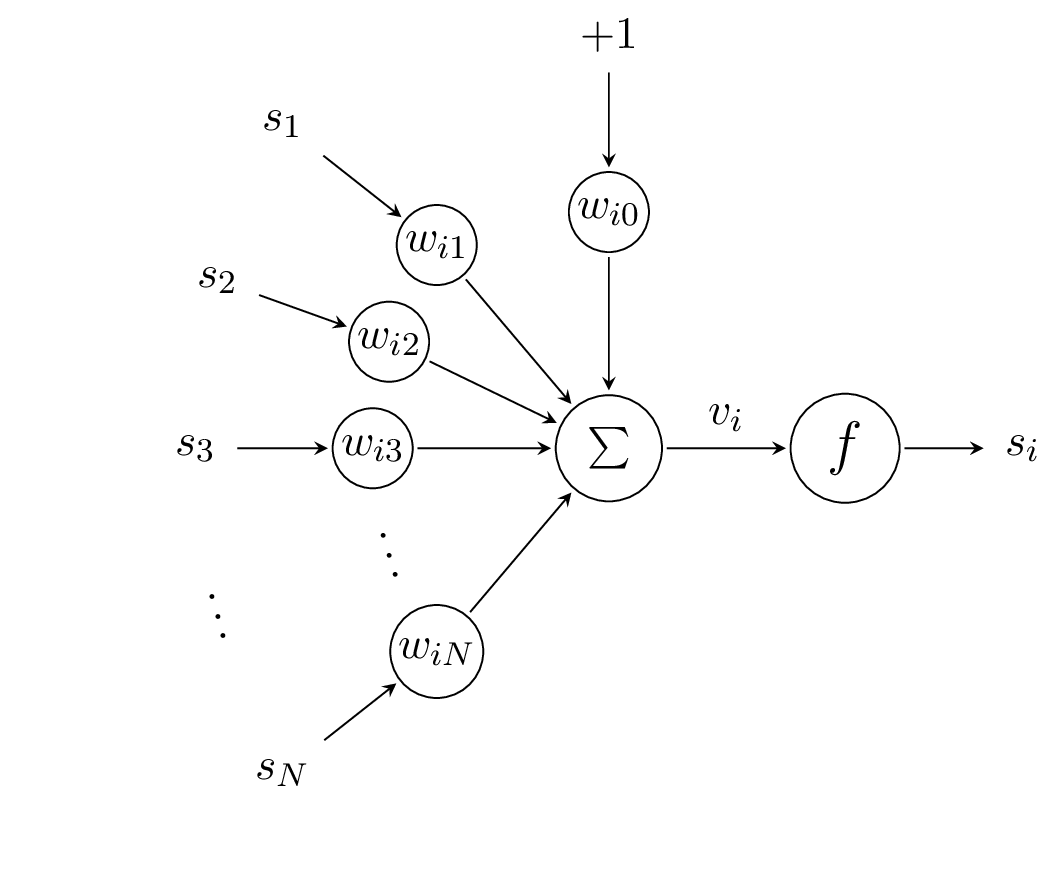
\includegraphics[width=.6\textwidth]{figures/fig_neurona/neurona.pdf}
\shorthandoff{<}
\shorthandoff{>}
\tikzsetnextfilename{figures/neurona/neurona}
\begin{tikzpicture}[   % opciones por defecto
  shorten >=1pt,     % acortar la linea en 1pt al final
  shorten <=1pt,     % acortar la linea en 1pt al principio
  - stealth,         % estilo de flecha al final (manual pgf p~210)
  draw=black!100,    % linea negro 100%
  %font=\relscale{0.9}\sffamily
]
  \tikzstyle{weight}=[draw, circle, inner sep=1pt];
  \tikzstyle{guide}=[draw=red!50];
  %
  %\draw[guide] ([shift={(90:5.5)}]7,0) arc (90:270:5.5);
  % arco que contiene las entradas
  \path ([shift={(150:5.5)}]7,0) arc (150:210:5.5)
  node [pos=0]    (s1) {$s_{1}$}
  node [pos=0.25] (s2) {$s_{2}$}
  node [pos=0.5]  (s3) {$s_{3}$}
  node [sloped, allow upside down, pos=0.75] {$\ldots$}
  node [pos=1]    (sN) {$s_{N}$};
  %% % arco que contiene las entradas
  %% \path ([shift={(135:4)}]5,0) arc (135:225:4)
  %%   node [pos=0]    (s1) {$s_{1}$}
  %%   node [pos=0.25] (s2) {$s_{2}$}
  %%   node [pos=0.5]  (s3) {$s_{3}$}
  %%   node [sloped, allow upside down, pos=0.75] {$\ldots$}
  %%   node [pos=1]    (sN) {$s_{N}$};
  %% %
  %\draw[guide] ([shift={(90:3)}]6,0) arc (90:270:3);
  % arco que contiene los pesos
  \path ([shift={(145:3)}]6,0) arc (145:215:3)
  node [weight,pos=0]    (w1) {$w_{i1}$}
  node [weight,pos=0.25] (w2) {$w_{i2}$}
  node [weight,pos=0.5]  (w3) {$w_{i3}$}
  node [sloped, allow upside down, pos=0.75] {$\ldots$}
  node [weight,pos=1]    (wN) {$w_{iN}$};
  %
  %% % arco que contiene los pesos
  %% \path ([shift={(135:2.2)}]5,0) arc (135:225:2.2)
  %%   node [weight,pos=0]    (w1) {$w_{i1}$}
  %%   node [weight,pos=0.25] (w2) {$w_{i2}$}
  %%   node [weight,pos=0.5]  (w3) {$w_{i3}$}
  %%   node [sloped, allow upside down, pos=0.75] {$\ldots$}
  %%   node [weight,pos=1]    (wN) {$w_{iN}$};
  %% %
  % nodo suma  
  \node [draw, circle, font=\LARGE] (sum) at (5,0) {$\sum$};
  %
  % conexiones entrada - peso y peso - suma
  \foreach \w in {1,2,3,N} {
    \path (s\w) edge (w\w);
    \path  (w\w) edge (sum);
  }
  %
  % peso umbral
  %\draw[guide] ([shift={(180:3)}]5,-1) arc (180:0:3);
  \path ([shift={(90:3)}]5,-1) node [weight] (w0) {$w_{i0}$};
  %% \path ([shift={(90:1.5)}]5,0) node [weight] (w0) {$w_{i0}$};
  \draw[] (w0) -- (sum);
  %
  % entrada +1
  %\draw[guide] ([shift={(180:5.5)}]5,-2) arc (180:0:5.5);
  \path ([shift={(90:5.5)}]5,-2) node [] (plus1) {$+1$};
  \draw[] (plus1) -- (w0);
  %
  % funcion activacion
  %\draw[guide] ([shift={(90:3)}]4,0) arc (90:-90:3);
  \node [draw, circle, font=\large] (fun) at (7,0) {$f$};
  \draw[] (sum) -- (fun) node [pos=0.5, above] {$v_i$};
  %
  % salida s_i
  %\draw[guide] ([shift={(90:5.5)}]3,0) arc (90:-90:5.5);
  \node [] (out) at (8.5,0) {$s_i$};
  \draw[] (fun) -- (out);
  %
  % nodo vacio para separar imagen
  \node at (0,-3.5) {};
\end{tikzpicture}
\shorthandon{<}
\shorthandon{>}


\caption{\captionStyle\protect\label{fig:neurona} El modelo de una neurona.}
\end{figure}
%
%
\subsection{La arquitectura del perceptrón multicapa}
%
El perceptrón multicapa tiene una arquitectura acíclica organizada en
\e{capas}.
La primer capa se denomina \e{capa de entrada} y contiene, en lugar de
neuronas, nodos sensores que ``leen'' el vector presentado como
entrada a la red.
Los valores de las salidas de esta capa equivalen a los componentes
del vector.
Las capas subsiguientes contienen neuronas, cada una de las cuales
recibe como entrada \e{todas} las salidas de la capa anterior.
Para el cálculo de las salidas de cada capa se requiere conocer los
valores de las salidas de la capa anterior, por lo que se dice que el
vector de entrada se \e{propaga hacia adelante} a través de la red.

La salida global de la red se compone por las salidas de las neuronas
en la última capa, denominada simplemente \e{capa de salida}.
Las capas que no son ni de entrada ni de salida se denominan \e{capas
  ocultas}.

En la \iflatexml{}Figura~\ref{fig:mlp}\else\autoref{fig:mlp}\fi{} se
representa un perceptrón multicapa de 2 capas, que lee a su entrada un
vector de 3 elementos.
Este vector es propagado a través de una capa oculta de 4 neuronas
hasta alcanzar las 2 neuronas en la capa de salida, que determinan la
salida de la red.

\begin{figure}[H]
\figureStyle
% 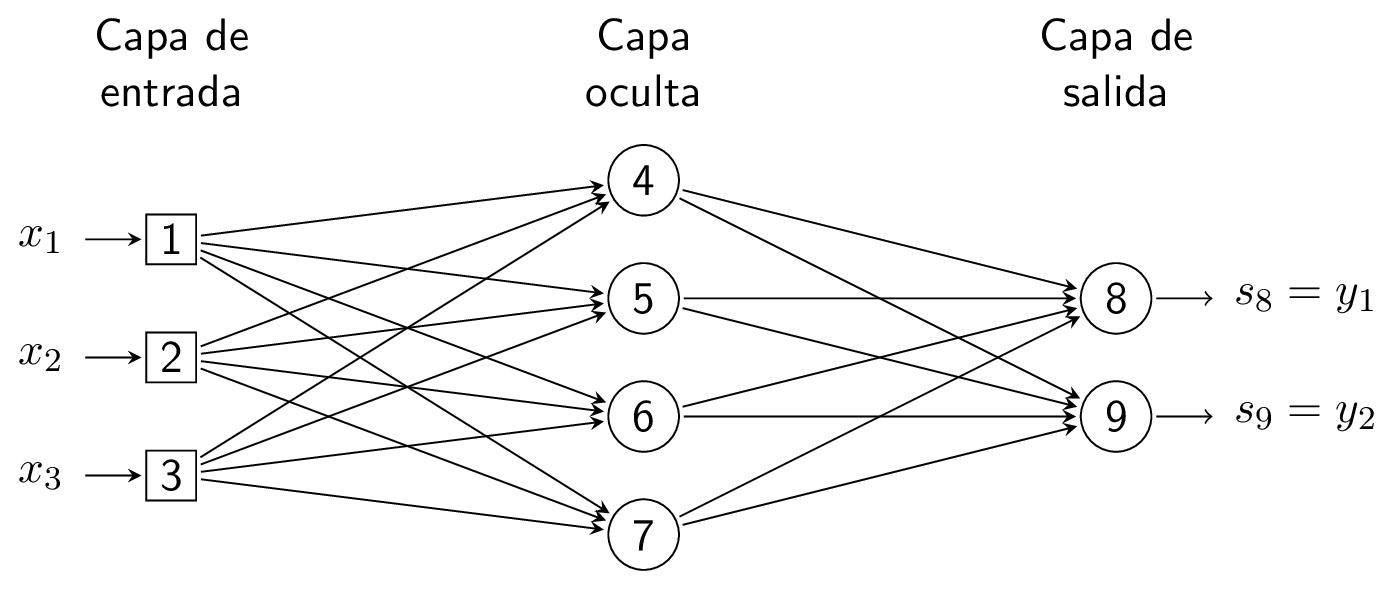
\includegraphics[width=.8\textwidth]{figures/fig_mlp/mlp.pdf}
\def\layersep{4cm}
\def\inputbegin{1}
\def\inputend{3}
\def\hiddenbegin{4}
\def\hiddenend{7}
\def\outputbegin{8}
\def\outputend{9}

\shorthandoff{<}
\shorthandoff{>}
\tikzsetnextfilename{figures/mlp/mlp}
\begin{tikzpicture}[   % opciones por defecto
    shorten >=1pt,     % acortar la linea en 1pt al final
    shorten <=1pt,     % acortar la linea en 1pt al principio
    - stealth,         % estilo de flecha al final (manual pgf p~210)
    draw=black!100,    % linea negro 100%
    node distance=\layersep, % no se que hace esto
    font=\relscale{0.9}\sffamily
  ]

  \tikzstyle{every pin edge}=[stealth -,shorten <=1pt]
  \tikzstyle{neuron}=[draw, minimum size=17pt,inner sep=0pt]
  \tikzstyle{input neuron}=[neuron, minimum size=12pt];
  \tikzstyle{output neuron}=[neuron, circle];
  \tikzstyle{hidden neuron}=[neuron, circle];
  \tikzstyle{annot} = [text width=4em, text centered]

    % Draw the input layer nodes
    \foreach \name / \y in {\inputbegin,...,\inputend}
    % This is the same as writing \foreach \name / \y in {1/1,2/2,3/3,4/4}
        \node[input neuron, pin=left:{$x_\y$}] (N-\name) at (0,-\y) {\y};

    % Draw the hidden layer nodes
    \foreach \name / \y in {\hiddenbegin,...,\hiddenend}
        \path[yshift=\hiddenbegin cm - 0.5cm]
        node[hidden neuron] (N-\name)
        at (\layersep,-\y cm) {\y};

    % Draw the output layer nodes
        \foreach \name[count=\mycount from 1] / \y in {\outputbegin,...,\outputend}
        \path[yshift=\outputbegin cm - 1.5cm]        
        node[output neuron,pin={[pin edge={->}]right:{$s_\y=y_\mycount$}},%
              right of=H-3] (N-\name) at (\layersep,-\y){\y};

    % Connect every node in the input layer with every node in the
    % hidden layer.
    \foreach \source in {\inputbegin,...,\inputend}
        \foreach \dest in {\hiddenbegin,...,\hiddenend}
            \path (N-\source) edge (N-\dest);

    % Connect every node in the hidden layer with the output layer
    \foreach \source in {\hiddenbegin,...,\hiddenend}
        \foreach \dest in {\outputbegin,...,\outputend}
            \path (N-\source) edge (N-\dest);

    % Annotate the layers
    \node[annot,above of=N-\hiddenbegin, node distance=1cm] (hl) {Capa oculta};
    \node[annot,left of=hl] {Capa de entrada};
    \node[annot,right of=hl] {Capa de salida};
    \node[annot] at (0,-4) {};
\end{tikzpicture}
\shorthandon{<}
\shorthandon{>}


\caption{\captionStyle\protect\label{fig:mlp} Perceptrón multicapa.
}
\end{figure}
%
%
\subsection{Entrenamiento}
%
El objetivo del entrenamiento en el perceptrón multicapa es ajustar
los pesos de la red de forma que ésta efectúe la transformación
expresada por el conjunto de entrenamiento $D=(\xx(n),\yy(n))$,
$n=1,\ldots,\ell$.
La diferencia entre las salidas deseadas y las salidas efectivas de la
red se mide con la función de \e{energía} del error $E$:
%
\begin{align}\label{e2:energy-function}
  E = \frac{1}{2}\sum_{j=1}^{\ell}\|\yy_j-\hat{\yy}_j\|,
\end{align}
%
en donde $\hat{\yy}_j$ es el vector formado con las salidas de cada
neurona de la capa de salida.
La función $E$ puede interpretarse como una medida de {aptitud} de los
pesos de la red al conjunto $D$, de modo que satisfacer el objetivo
del aprendizaje es equivalente a encontrar un mínimo global de $E$.
La discusión a continuación se basa en aquella presentada en
\cite[Capítulo~4]{haykin}.

Considerando una neurona $i$ en la capa de salida, sea $s_i(n)$ la
salida de la misma en respuesta al estímulo $\xx(n)$ aplicado en la
capa de entrada.
La \e{señal de error} producida en la salida de esta neurona viene
dada por
%
\begin{align}\label{e2:error-signal-neuron} %4.2
  e_i(n)=y_{k}(n)-s_{i}(n)
\end{align}
%
en donde $y_k(n)$ es la componente del vector de respuesta deseada
$\yy(n)$ correspondiente a la posición de la neurona $i$ en la capa de
salida.
%% en donde $y_{i}$ es el $i$-ésimo elemento del vector de respuesta
%% deseada $\yy$.
La \e{energía de error instantáneo} de la neurona $i$ se define según
%
\begin{align}\label{e2:error-energy-neuron} %4.3
  \C{E}_i(n)=\frac{1}{2}e^2_i(n).
\end{align}
%
Sumando las contribuciones error-energía de todas las neuronas en la
capa de salida, se expresa la \e{energía total de error instantáneo}
de la red como
%
\begin{align}\label{e2:error-energy-net} %4.4
  \C{E}(n)&=\sum_{i\in C}\C{E}_i(n) \\
  &=\frac{1}{2}\sum_{i\in C}e^2_i(n).
\end{align}
%
Aquí, el conjunto $C$ contiene los índices de las neuronas en la capa
de salida.
La energía de error promedio sobre el conjunto de entrenamiento viene
dada por
%
\begin{align}\label{e2:average-energy-net} %4.5
  \C{E}_{\T{av}}&=\frac{1}{\ell}\sum_{n=1}^\ell\C{E}(n) \\
  \tab=\frac{1}{2\ell} \sum_{n=1}^\ell \sum_{i\in C}e^2_i(n).
\end{align}
%
Naturalmente, tanto la energía de error instantáneo como la energía de
error promedio son funciones de todos los pesos sinápticos de la red.
Esta dependencia funcional no fue incluida de forma explícita en la
definición de $\C{E}(n)$ y $\C{E}_{\T{av}}$ en pos de simplificar la
notación.

%
\subsubsection{Aprendizaje en línea y aprendizaje por época}
%
El aprendizaje en línea y el aprendizaje por época hacen referencia
a dos estrategias de entrenamiento que difieren según
el momento en que se efectúa la actualización de los pesos de la
red:
%
\begin{itemize}
\item En el aprendizaje en línea, o aprendizaje por patrón, se efectúa una
  actualización de los pesos de la red inmediatamente
  luego de calcular la salida y el
  error instantáneo de cada ejemplo del conjunto de aprendizaje.
  Esto implica que se efecúan tantas actualizaciones como ejemplos haya
  en el conjunto de entrenamiento.
  Este método funciona especialmente bien
  para grandes conjuntos de entrenamiento que contengan información
  redundante.
\item En el aprendizaje por época (\e{batch learning}),
  la actualización de los pesos de la red
  se efectúa una vez que han sido calculadas las salidas de todos los
  patrones en el conjunto de entrenamiento, minimizando la función de
  error promedio $\C{E}_{\T{av}}$.
\end{itemize}
%
Mientras que el aprendizaje en línea resulta idóneo para situaciones en donde
se requiere una adaptación continua de la máquina de aprendizaje, el
aprendizaje por época redunda en superficies de error más estables, ya que
se promedia todo el conjunto de datos.
En el presente trabajo, se considera en todos los casos el aprendizaje
por época.

%% Los procedimientos adaptativos descritos en adelante
%% utilizan este tipo de aprendizaje, ya que la información de gradiente
%% sumada contiene información más fiable acerca de la forma de la
%% función de error como un todo \cite{riedmiller}.  Algunos autores, sin
%% embargo, sugieren que la mejor técnica es la del aprendizaje en línea
%% \cite{haykin}.

%% %
%% \subsubsection{Técnicas adaptativas}
%% %
%% A la fecha, se han propuesto muchas técnicas para afrontar los
%% problemas inherentes del método de descenso por gradiente. La mayoría
%% tienen sus bases de la disciplina de la teoría de
%% optimización.

%% Estas técnicas se pueden dividir en dos
%% categorías. Aquellos algoritmos que utilizan un conocimiento global
%% del estado de la red como un todo, tal como la dirección del vector de
%% actualización de los pesos ``entero'', son llamadas técnicas globales.
%% Existen muchos ejemplos donde los algoritmos de aprendizaje utilizan el
%% conocimiento global \cite{salomon,moeller}.

%% Por contraste, las estrategias de adaptación locales se basan
%% únicamente en información específica a los pesos, tal como el
%% comportamiento temporal de la derivada parcial de este peso. El
%% enfoque local se relaciona más naturalmente con el concepro de
%% procesamiento distribuido en el que los cálculos pueden efectuarse en
%% paralelo.  Más aún, en muchos casos se encuentra que las estrategias
%% locales funcionan mucho mejor que las globales, a pesar del hecho que
%% utilizan menos información y de que normalmente son mucho más rápidas
%% y fáciles de calcular \cite{schiffmann}.

%
%
\subsection{El algoritmo de retropropagación}
%
El algoritmo de retropropagación es la forma básica de entrenamiento
del perceptrón multicapa, y se basa en ajustar progresivamente los
pesos $w_{ij}$ de la red a partir de la información del gradiente de
la función de error $\nabla\C{E}(n)$.
En cada iteración $n=1,\ldots,\ell$ el algoritmo calcula el error
instantáneo $\C{E}(n)$ de la red sobre el ejemplo $(\xx(n),\yy(n))$, y
aplica una corrección $\Delta{}w_{ij}(n)$ a los pesos sinápticos
$w_{ij}$ proporcional a la derivada parcial
$\dpar{\C{E}(n)}{w_{ij}}{}$.
% Esta forma de entrenamiento se llama \e{entrenamiento en línea}.

Según la regla de la cadena, la derivada $\dpar{\C{E}(n)}{w_{ij}}{}$
puede escribirse
%
\begin{align}\label{e2:deriv-E-wrt-w-expanded}
  \dpar{\C{E}(n)}{w_{ij}}{} = \dpar{\C{E}(n)}{s_i(n)}{}
  \dpar{s_i(n)}{v_i(n)}{} \dpar{v_i(n)}{w_{ij}}{}.
\end{align}
%
Diferenciando ambos lados de (\ref{e2:error-energy-neuron}) respecto
de $s_i(n)$, se tiene
%
\begin{align}\label{e2:deriv-E-wrt-s}
  \dpar{\C{E}(n)}{s_i(n)}{} = -e_i(n).
\end{align}
%
Por (\ref{e2:neuron-general}), se tiene
%
\begin{align}\label{e2:deriv-s-wrt-v}
  \dpar{s_i(n)}{v_i(n)}{} \tab = f'(v_i(n)),\tabs
  \dpar{v_i(n)}{w_{ij}}{} \tab = s_j(n).
\end{align}
%
Reemplazando (\ref{e2:deriv-E-wrt-s})--(\ref{e2:deriv-s-wrt-v}) en
(\ref{e2:deriv-E-wrt-w-expanded}), se tiene
%
\begin{align}\label{e2:deriv-E-wrt-w}
  \dpar{\C{E}(n)}{w_{ij}}{} = -e_i(n) f'(v_i(n)) s_j(n).
\end{align}
%
Cuando la neurona $i$ está en la capa de salida, esta fórmula se
utiliza directamente para el cálculo de $\dpar{\C{E}(n)}{w_{ij}}{}$,
ya que la señal de error $e_i(n)$ de la neurona viene dada por la
diferencia entre el valor deseado $y_k(n)$ y la salida de la neurona
$s_i(n)$ según (\ref{e2:error-energy-neuron}).

Cuando la neurona $i$ se ubica en una capa oculta, el cálculo de
$\dpar{\C{E}(n)}{w_{ij}}{}$ resulta más complejo, ya que no existe una
``respuesta deseada'' correspondiente $y_k(n)$.
Para calcular la derivada $\dpar{\C{E}(n)}{s_{i}}{}$ correspondiente a
una neurona oculta $i$, se supone que el valor de
$\dpar{\C{E}(n)}{s_r}{}$ es conocido para todas las neuronas $r$ de la
capa siguiente a la neurona $i$.
Si $\C{S}(i)$ contiene los índices $r$ de estas neuronas, se puede ver
que
%
\begin{align}
  \dpar{\C{E}}{s_i}{} \tab= \sum_{r\in\C{S}(i)}
      \dpar{\C{E}}{s_r}{}\dpar{s_r}{s_i}{} \notag\\
    \tab= \sum_{r\in\C{S}(i)}
      \dpar{\C{E}}{s_r}{}\dpar{s_r}{v_r}{}\dpar{v_r}{s_i}{} \notag\\
    \tab= \sum_{r\in\C{S}(i)} \dpar{\C{E}}{s_r}{} s'(v_r) w_{ri}.
    \label{e2:deriv-E-wrt-s-hid}
\end{align}
%
Reemplazando (\ref{e2:deriv-E-wrt-s-hid}) y (\ref{e2:deriv-s-wrt-v})
en (\ref{e2:deriv-E-wrt-w-expanded}), se tiene entonces
%
\begin{align}\label{e2:deriv-E-wrt-w-hid}
  \dpar{\C{E}(n)}{w_{ij}}{} =
  \sum_{r\in\C{S}(i)} \dpar{\C{E}(n)}{s_r(n)}{} s'(v_r(n)) w_{ri}
  f'(v_i(n)) s_j(n).
\end{align}
%
Esta fórmula es la clave del algoritmo de retropropagación: por la
arquitectura del perceptrón multicapa, la salida $s_i(n)$ de una
neurona oculta ejerce una influencia en la salida de todas las
neuronas en las capas posteriores.
Similarmente, el \e{gradiente local} de la señal de error de la
neurona viene determinado por los gradientes de error de todas las
neuronas en las capas subsiguientes.

Comenzando el cálculo de $\dpar{\C{E}(n)}{w_{ij}}{}$ por la capa de
salida (\ref{e2:deriv-E-wrt-w}) y continuando con las capas ocultas en
orden inverso (\ref{e2:deriv-E-wrt-w-hid}), el gradiente resulta
calculable para todas las neuronas.
Éste es el origen del nombre ``retropropagación'': se dice que la
información del gradiente de error se propaga hacia atrás, desde la
capa de salida hasta la primer capa oculta.
El desarrollo del algoritmo de retropropagación a mediados de los años
$80$ representó un hito en el campo de las redes neuronales, ya que
brindó un método computacionalmente eficiente para entrenar el
perceptrón multicapa \cite{haykin}.

En pos de simplificar la notación, la descripción del algoritmo de
retropropagación se ha efectuado siguiendo una estrategia de
aprendizaje \e{en línea}, en la que en cada iteración $n$ se presenta
un ejemplo $(\xx(n),\yy(n))$, se calcula la salida de la red
$\hat{\yy}(n)$ y se ajustan los pesos $\ww_{ij}$ según la derivada del
error instantáneo $\C{E}(n)$.
Otra estrategia de entrenamiento posible es el aprendizaje \e{por
  época} (en inglés \e{batch learning}), que consiste en ajustar los
pesos de la red a partir de la derivada de la función de error
promedio $\C{E}_{\T{av}}$.
Para ello, en cada iteración $t$ se obtienen las salidas de la red
para todo el conjunto de entrenamiento $D$, luego se calcula la
función de error promedio, y finalmente se ajustan los pesos
$\ww_{ij}$ de la red en proporción a la derivada
$\dpar{\C{E}_{\T{av}}(t)}{w_{ij}}{}$.

%
\subsubsection{Ajuste de los pesos de la red}
%
En el caso del entrenamiento en línea, en cada paso del entrenamiento
$t$ se calcula la respuesta de la red
$\B{s}(t)$ para la entrada $\xx(t)$ y luego se calcula el gradiente
$\dpar{\C{E}(t)}{w_{ij}}{}$ propagando hacia atrás la señal de error $\C{E}(t)$.
A partir de la información del gradiente
se aplica una corrección $\Delta{}w_{ij}(t)$ sobre el peso
$w_{ij}(t)$, según la ``regla delta''
%
\begin{align}
\label{e2:delta-rule}
  \Delta w_{ij}(t)\tab=-\eta\dpar{\C{E}(t)}{w_{ij}}{},
\end{align}
%
en donde $\eta$ es el parámetro \e{velocidad de aprendizaje} del
algoritmo de retropropagación. La utilización del signo menos en la
\iflatexml{}Ecuación~\ref{e2:deriv-E-wrt-w}
\else\autoref{e2:deriv-E-wrt-w}\fi{} indica el \e{descenso por
  gradiente} en el espacio de los pesos $w_{ij}$. Esto implica que el
ajuste efectuado modifica los pesos en la dirección que reduce el
valor de $\C{E}(t)$.

%
\subsubsection{Entrenamiento por época}
%
En una estrategia de entrenamiento por época, en cada iteración $t$
se propagan hacia adelante todos los vectores $\xx(n)$ del conjunto
de entrenamiento $D$, y a partir de los respectivos
gradientes de error instantáneo $\dpar{\C{E}(n)}{w_{ij}}{}$
se obtiene la energía de error promedio $\C{E}_{\T{av}}$
(\iflatexml{}Ecuación~\ref{e2:average-energy-net}\else\autoref{e2:average-energy-net}\fi)
para la época $t$.

El gradiente de error promedio para la época viene dado por
%
\begin{align}\label{e2:deriv-Eav-wrt-w}
  \dpar{\C{E}_{\T{av}}(t)}{w_{ij}}{}\tab=
  \frac{1}{\ell}\sum_{n=1}^\ell\dpar{\C{E}(n)}{w_{ij}}{},
\end{align}
%
y la corrección a aplicar a los pesos viene dada por
%
\begin{align}\label{e2:delta-rule-epoch}
  \Delta w_{ij}(t)\tab=-\eta\dpar{\C{E}_{\T{av}}(t)}{w_{ij}}{}.
\end{align}
%
Dado que la función $\C{E}_{\T{av}}$ promedia todos los patrones de la
época, la superficie de la función de error resultante es más
``suave'' y el gradiente $\nabla\C{E}_{\T{av}}$ es numéricamente más
estable que en el caso del error intantáneo.

%
\subsubsection{Criterio de corte}
%
En general, no existe un criterio de corte bien definido para
detener el entrenamiento. Algunos criterios razonables para establecer
la convergencia pueden ser:
%
\begin{itemize}
\item Cuando la norma del gradiente es muy pequeña
  ($\|\nabla\C{E}\|\leq\epsilon$), probablemente se deba a que se
  alcanzó un mínimo local de la función de error.
\item Cuando la función de energía promedio $\C{E}_{\T{av}}$ varía muy
  poco entre épocas, también podría significar que se alcanzó un
  mínimo local, indicando convergencia.
\end{itemize}
%
El problema de estos criterios es similar al de la velocidad de
aprendizaje: los valores de tolerancia a considerar para la
convergencia serán siempre dependientes del problema, y una elección
incorrecta puede llevar ya sea a un corte prematuro del entrenamiento,
o bien a que el algoritmo nunca converja.

Un criterio de convergencia alternativo, ampliamente utilizado, se
basa en la aplicación del método de retención sobre el conjunto de
entrenamiento $D$, entrenando sobre un conjunto de estimación $E$ y
evaluando en cada iteración el error sobre un conjunto de validación
$V$ que estima el error de generalización.  El entrenamiento se
detiene cuando se observa que este error es adecuado, o bien cuando
resulta evidente que ha alcanzado su mínimo.

%
\subsection{Variantes del algoritmo de retropropagación}
%
Las técnicas descriptas a continuación son variantes del algoritmo de
retropropagación que intentan sortear algunas de las dificultades
inherentes al descenso por gradiente de la función de error mediante
la utilización de reglas alternativas para la actualización de los
pesos de la red.
En adelante, se utiliza la notación $\C{E}(t)$ para indicar la función
de error, y se observa que para el caso del entrenamiento por época
$\C{E}(t)$ refiere simplemente a $\C{E}_{av}(t)$.

%
\subsubsection{Término de momento}
%
Una estrategia propuesta para incrementar la velocidad de aprendizaje
y mejorar la estabilidad del algoritmo de retropropagación consiste en
modificar la regla delta
(\iflatexml{}Ecuación~\ref{e2:delta-rule}\else\autoref{e2:delta-rule}\fi)
añadiendo un \e{término de momento}
%
\begin{align}\label{e2:momentum-term}
  \Delta w_{ij}(t)\tab=-\eta\dpar{\C{E}(t)}{w_{ij}}{} +\mu\Delta
  w_{ij}(t-1).
\end{align}
%
El término de momento simplemente añade una fracción $\mu$ del paso
anterior $t-1$ al paso actual $t$: si el gradiente mantiene su
orientación, el efecto del término de momento es aumentar la velocidad
de aprendizaje; si en cambio el gradiente cambia de dirección, el
momento ``suaviza'' las oscilaciones.
El \hparam{} de momento $0<\mu<1$ se determina mediante prueba y error
para cada problema.

%
\subsubsection{Descenso más pronunciado}
%
%% En la ``regla delta'' básica
%% (\iflatexml{}Ecuación~\ref{e2:delta-rule}\else\autoref{e2:delta-rule}\fi),
%% la dirección de búsqueda del mínimo
%% viene dada por el negativo del gradiente
%% $-\nabla\C{E}(n)=-\dpar{\C{E}(n)}{w_{ij}}{}$, mientras que la
%% velocidad de aprendizaje $\eta$ determina la magnitud del paso a
%% efectuar.
La regla llamada del \e{descenso más pronunciado} consiste
en buscar, en cada iteración, una velocidad de aprendizaje óptima
$\eta(t)$ mediante una estrategia iterativa denominada \e{búsqueda en
  la línea}.
Básicamente, la búsqueda en la línea consiste en evaluar
la función de error resultante para distintos $\eta$ hasta encontrar
el óptimo.
La regla de actualización de los pesos para esta estrategia es
%
\begin{align}\label{e2:delta-rule-steepest}
  \Delta w_{ij}(t)\tab=-\eta(t)\nabla{\C{E}(t)}.
\end{align}
%
La optimización de $\eta(t)$ añade complejidad computacional a cada
iteración, aunque en general resulta en una reducción del número de
iteraciones necesarias hasta alcanzar la convergencia.
Desde el punto de vista del usuario, evita la necesidad de determinar
el parámetro de entrenamiento $\eta$ mediante prueba y error.

%
\subsubsection{Gradiente conjugado}
%
Al utilizar la regla del descenso más pronunciado, puede demostrarse
que dos pasos de actualización sucesivos ocurren necesariamente en
direcciones perpendiculares.  Esta perpendicularidad entre iteraciones
genera un ``zigzagueo'' en el camino del descenso del gradiente. El
algoritmo del \e{gradiente conjugado} aprovecha esta perpendicularidad
estableciendo como dirección de búsqueda una combinación de la
dirección de búsqueda anterior y del gradiente actual, ``atravesando''
el zigzag y logrando entonces pasos más pronunciados y directos.  La
regla de actualización de los pesos mediante gradiente conjugado viene
dada por
%
\begin{align}\label{e2:delta-rule-conjugate}
  \Delta w_{ij}(t)\tab=\eta(t)\B{d}(t), \tabs
  \B{d}(t)\tab=-\nabla{\C{E}(t)}+\beta\B{d}(t-1),
\end{align}
%
donde $\eta(t)$ se determina mediante búsqueda en la línea y $\beta$
viene dado por la fórmula de Polak-Ribière:
%
\begin{align}\label{e2:polak-ribiere}
  \beta=
  \frac{(\nabla{\C{E}(t)}-\nabla{\C{E}(t-1)})\nabla{\C{E}(t)}}{(\nabla{\C{E}(t-1)})^2}.
\end{align}
%
El mayor costo computacional de las iteraciones en el algoritmo del
gradiente conjugado se compensa con una convergencia mucho más rápida
en problemas de clasificación binarios en comparación con la
retropropagación clásica.

%
\subsubsection{Gradiente conjugado escalado}
%
La estrategia del gradiente conjugado escalado (\e{scaled conjugate
  gradient, SCG}) \cite{scg} es una mejora de la estrategia del
gradiente conjugado estándar que evita la necesidad de optimizar
$\eta(t)$ en cada iteración, ya que determina el paso óptimo a partir
de una aproximación de la segunda derivada de la función $\C{E}$.
Los detalles de la derivación del método pueden encontrarse en
\cite{scg}.
En la actualidad, el algoritmo SCG es una de las estrategias de
entrenamiento más utilizadas debido a su estabilidad y velocidad de
entrenamiento.

%
\subsubsection{Rprop}
%
El algoritmo Rprop \cite{rprop} es una variante heurística sencilla
del algoritmo de retropropagación clásico, que actualiza cada uno de
los pesos de la red de forma independiente.
%% A diferencia de los
%% algoritmos vistos anteriormente, Rprop considera únicamente el signo
%% del gradiente para cada peso, ignorando su magnitud.
Para cada peso $w_{ij}$, Rprop determina un valor de actualización
específico $\Delta{}w_{ij}$ según la siguiente regla basada en el
signo de la derivada parcial
%
\begin{align}
  \Delta{}w_{ij}(t) =
  \begin{cases}
    -\Delta_{ij}^{(t)}, & \T{si}\,\,\,\dpar{\C{E}}{w_{ij}}{}(t) > 0, \\
    +\Delta_{ij}^{(t)}, & \T{si}\,\,\,\dpar{\C{E}}{w_{ij}}{}(t) < 0, \\
    0, & \T{en otro caso}.
  \end{cases}
\end{align}
%
El algoritmo regula su funcionamiento mediante dos hiperparámetros,
$\Delta_0$ y $\Delta_{\max}$, que especifican respectivamente el valor
de inicialización de todos los $\Delta_{ij}$ y la magnitud máxima
permitida para cada $\Delta_{ij}$.
Los valores de cada $\Delta_{ij}$ se modifican en cada iteración según
la regla
%
\begin{align}
  \Delta{}_{ij}^{(t)} \tab =
  \begin{cases}
    \eta^+\,\Delta_{ij}^{(t-1)}, & \T{si}\,\,\,\dpar{\C{E}}{w_{ij}}{} {(t-1)}
      \dpar{\C{E}}{w_{ij}}{} {(t)} > 0, \\
    \eta^-\,\Delta_{ij}^{(t-1)}, & \T{si}\,\,\,\dpar{\C{E}}{w_{ij}}{} {(t-1)}
      \dpar{\C{E}}{w_{ij}}{} {(t)} < 0, \\
    \Delta_{ij}^{(t-1)}, & \T{en otro caso}.
  \end{cases}
  \tabs
  \begin{split}
    \eta^-=0.5, \\
    \eta^+=1.2.
  \end{split}
\end{align}
%
El algoritmo Rprop es una de las técnicas más rápidas y más populares
para el entrenamiento del perceptrón multicapa.
Dada su estabilidad, la elección de los hiperparámetros $\Delta_{0}$ y
$\Delta_{\max}$ no es crítica, y en la práctica se utilizan los
valores preestablecidos $\Delta_{0}=0.1$ y $\Delta_{\max}=50$.

%
%
%
\section{Máquina de vectores de soporte}
%
La máquina de vectores de soporte (\eng{Support Vector Machine, SVM})
es una máquina de aprendizaje propuesta por Boser et al. \cite{boser}
y Cortes y Vapnik \cite{svm} que puede ser utilizada para tareas de
clasificación y regresión. Su funcionamiento se basa en la
construcción de un modelo en el cual los ejemplos son representados
como puntos en el espacio.
En un problema de clasificación, el entrenamiento de la SVM construye,
a partir de los ejemplos en el conjunto de entrenamiento, una frontera
de decisión que permite determinar la pertenencia de clase de los
ejemplos según se ubiquen a un lado u otro de la frontera.

La popularidad de la máquinas de vectores de soporte se debe en gran
parte a que permiten incorporar no-linealidad a la representación
vectorial de los ejemplos de manera eficiente, mediante la utilización
de familias especiales de funciones denominadas núcleos.

%% En su variante más común, la máquina de vectores de soporte incorpora
%% un término de regularización que permite su aplicación a conjuntos de
%% datos no separables y reducir la complejidad de la solución, evitando
%% el sobreajuste.

La máquina de vectores de soporte es un tipo de \e{clasificador
  lineal} con tres propiedades importantes:
%
\begin{enumerate}
\item El algoritmo de entrenamiento de la SVM genera una frontera de
  decisión óptima desde el punto de vista geométrico.
\item Permite efectuar cálculos entre los vectores (ejemplos) de
  manera eficiente mediante la utilización de funciones especiales
  denominadas \e{núcleos}.
\item Permite incorporar regularización al modelo, que evita el
  sobreajuste y al mismo tiempo permite aplicar el clasificador a
  datos no separables.
\end{enumerate}
%
A continuación se presenta una descripción de la SVM
comenzando por el clasificador lineal e incorporando estas propiedades
hasta alcanzar la formulación más general, que
utiliza funciones núcleo e incorpora regularización al modelo.
En esta descripción se trata la obtención del modelo de un
clasificador binario a partir de un conjunto de entrenamiento
$D=\left((\xx_1,y_1),\ldots,(\xx_\ell,y_\ell)\right)$, en donde el
indicador de clase del $i$-ésimo ejemplo toma alguno de los dos
valores posibles $y_i=+1$ o $y_i=-1$.

%
%
\subsection{El clasificador lineal}
%
El clasificador lineal es una máquina de aprendizaje \cite{nilsson}
que sirve como fundamento de la máquina de vectores de soporte. De
hecho, la SVM es en sí misma un tipo particular de
clasificador lineal.

En primer lugar, sea $\BPhi:X\rightarrow{}Z$ una función que
transforma el denominado \e{espacio de entrada} $X$ a otro espacio
vectorial inducido $Z$, denominado \e{espacio imagen}.
A partir del
conocimiento previo del problema, se pretende que la transformación
$\BPhi$ sea tal que los \e{vectores imagen} $\zz=\BPhi(\xx)$ se
ubiquen, según su clase $\yy$, en regiones del espacio $Z$ bien
diferenciadas entre sí.

Entonces, dado un patrón de entrada $\xx\in{}X$, el clasificador
lineal calcula primero el vector imagen $\zz=\BPhi(\xx)$, para luego
asignarle una clase de salida $\hat{y}=\pm{}1$ según sea el signo de
la función discriminante lineal $f=\ww^T\zz+b$. Los valores de $\ww$
y $b$ se determinan en el entrenamiento del clasificador, cuyos detalles
se omiten de la presente descripción.

Por último, se observa que la ecuación $\ww^T\zz+b=0$ define un
hiperplano en el espacio inducido $Z$. Dicho hiperplano determina una
frontera de decisión entre las clases $\hat{\yy}=+1$ e
$\hat{\yy}=-1$. Para visualizarlo, obsérvese que, desde el punto de
vista geométrico, el signo de $\ww^T\zz+b$ determina de qué lado del
plano se encuentra el punto $\zz$.
%
\begin{quote}
  {\bfseries Notación.}\quad{}En la literatura, resulta común
  encontrar que el vector $\zz$ se denomina \e{vector de
    características} (\e{feature vector}) y el espacio vectorial $Z$
  como \e{espacio de las características} (\e{feature space}).  En
  este trabajo se prefiere denominarlos con los nombres alternativos
  \e{vector imagen} y \e{espacio vectorial imagen} para evitar
  confusión con el proceso previo de extracción de características.
\end{quote}
%

%
\subsubsection{Espacio imagen}
%
La primera adición de la SVM al clasificador lineal básico es una
transformación de los vectores de entrada a un \e{espacio imagen}.
Esto se logra aplicando una función $\BPhi:X\rightarrow{}Z$, que
transforma el \e{espacio de entrada} $X$ a otro espacio vectorial
inducido $Z$, llamado \e{espacio imagen}.
La elección de la función $\BPhi$ es tal que los datos transformados
sean separables en el espacio $Z$.
Dada una entrada $\xx\in{}X$, la máquina de vectores de soporte
calcula un vector imagen $\BPhi(\xx)$ y le asigna una clase de
salida $\hat{y}=\pm{}1$ según
%
\begin{align*}
  y = \T{signo}(\ww^T \BPhi(\xx)+b)
\end{align*}
%
Los valores de $\ww$ y $b$ se obtienen del algoritmo de entrenamiento,
que se explicará más adelante.
En este caso, la frontera de decisión se ubica en el espacio imagen
$Z$, y viene dada por el hiperplano con ecuación
$\ww^T\BPhi(\xx)+b=0$.
%
\begin{quote}
  {\bfseries Notación.}\quad{}En la literatura, resulta común
  encontrar que el vector $\BPhi(\xx)$ se denomina \e{vector de
    características} (\e{feature vector}) y el espacio vectorial $Z$
  como \e{espacio de las características} (\e{feature space}).  En
  este trabajo se prefiere denominarlos con los nombres alternativos
  \e{vector imagen} y \e{espacio vectorial imagen} para evitar
  confusión con el proceso previo de extracción de características.
\end{quote}
%

%
%
\subsection{El hiperplano de separación óptimo}
%
Dado un conjunto de entrenamiento
$D=\left((\xx_1,y_1),\ldots,(\xx_\ell,y_\ell)\right)$, se dice que
éste es linealmente separable en el espacio imagen $Z$ cuando existe
una función discriminante lineal $f(\xx)=\ww^T\BPhi(\xx)+b$ tal que su
signo permite determinar sin errores la clase de todos los elementos
del conjunto. Cuando el conjunto $D$ es linealmente separable en $Z$,
se sabe que existen infinitas funciones discriminantes lineales
capaces de clasificar correctamente todos los elementos.

La característica saliente de la máquina de vectores de soporte es
que, durante el entrenamiento, determina un hiperplano de separación
$\ww^T\zz+b=0$ \e{óptimo}, que maximiza la distancia a los puntos
$\zz_i=\BPhi(\xx_i)$ más cercanos. Esto se expresa a través del
problema de optimización
%
\begin{equation}\label{e2:svm-problem-basic}
  \begin{aligned}
    \min_{\ww,b} \quad\tabs \frac{1}{2}\|\ww\|^2, \\
    \T{sujeto a}\quad\tabs y_i f_i\geq1,\,i=1,\ldots,\ell\,.
  \end{aligned}
\end{equation}
%
Aquí, $f_i=f(\xx_i)=\ww^T\BPhi(\xx_i)+b$ es la función discriminante
lineal aplicada al vector $\xx_i$. En términos coloquiales, este
problema puede leerse
%
\begin{align*}
  \min \frac{1}{2}\|\ww\|^2 \quad \tabs \T{encontrar el $\ww$ más
    pequeño según la norma euclídea $\|\cdot\|$}\ldots\\
  |f_i|\geq1 \quad \tabs \T{estableciendo en $1$ la distancia del
    hiperplano a los puntos más cercanos},\\
  y_i\hat{y}_i>0\quad \tabs \T{y tal que la clase $y_i$ coincida con el
    signo del discriminante ($\hat{y}_i=\T{signo}(f_i)$)}.
\end{align*}
%
La distancia de un vector $\zz_i=\BPhi(\xx_i)$ al hiperplano
$\ww^T\zz+b=0$ viene dada por
%
\begin{align*}
  d_i=\frac{\ww}{\|w\|}\cdot\zz_i+b,
\end{align*}
%
por
ello, minimizar $\|w\|$ equivale a maximizar la distancia $d_i$.

Puede demostrarse que el vector solución $\ww_*$ al
Problema~\ref{e2:svm-problem-basic} es una combinación lineal de
aquellos vectores $\zz_i$ para los cuales se cumpla la condición:
%
\begin{align*}
  |\ww^T\zz_i+b\,|=1.
\end{align*}
%
Estos vectores se denominan \e{vectores de soporte}, lo que da el
nombre al clasificador.
Los hiperplanos $\ww^T\zz+b=\pm1$ que contienen los vectores
de soporte conforman el llamado \e{margen} del clasificador.

El Problema~\ref{e2:svm-problem-basic} también puede entenderse como
la maximización de la distancia del hiperplano $\ww^T\zz+b=0$ al
margen $\ww^T\zz+b=\pm1$.
Esto explica el nombre alternativo por el cual se conoce a la máquina
de vectores de soporte: \e{clasificador de margen máximo}.

%% Desde el punto de vista numérico, el problema
%% (\ref{e2:svm-problem-basic}) es un problema de optimización cuadrático
%% convexo con restricciones lineales.

%
%
\subsection{Formulación dual}
%
En el problema (\ref{e2:svm-problem-basic}) se minimiza una función
cuadrática simple con restricciones relativamente complejas
${y}_i(\ww^T\BPhi(\xx_i)+b)\geq{}1$. Utilizando la técnica de los
multiplicadores de Lagrange \cite{bottou,kuhntucker}, resulta posible
obtener una fomulación alternativa del problema con restricciones
simples, cuya conveniencia será aparente con la introducción del
concepto de núcleos.

La técnica de los multiplicadores de Lagrange permite incorporar las
restricciones del problema dentro de la función a optimizar.  En
primer lugar, se define el funcional lagrangiano
%
\begin{align}\label{e2:lagrangian}
  \C{L}(\ww,b,\Balpha) = \frac{1}{2} \|\ww\|^2 + \sum_{i=1}^{\ell}
  \alpha_i (1-y_i(\langle\ww,\BPhi(\xx)\rangle+b)).
\end{align}
%
Como se puede ver, el funcional $\C{L}$ es la función a optimizar más
las restricciones ${y}_if_i\geq{}1$, expresadas en la forma $g(\xx)\leq0$,
y multiplicadas por las variables de holgura $\alpha_i$,
denominadas \e{multiplicadores de Lagrange}. A partir del lagrangiano
se plantea la formulación \emph{dual} del problema
%
\begin{align}\label{e2:svm-problem-dual}
  \begin{split}
    \max_\alpha \tabs\quad f(\Balpha) = \min_{\ww,b} \C{L}(\ww,b,\Balpha)\\
    \T{sujeto a} \tabs\quad \alpha_i \geq 0\T{ para todo } i\in\{1,\ldots,\ell\}.
  \end{split}
\end{align}
%
En este problema las restricciones son más sencillas y
aplican únicamente a los multiplicadores de Lagrange.
Dado que $\frac{1}{2}\|\ww\|^2$ es una función continuamente derivable
y convexa, y dado que $\C{L}$ es continuamente derivable respecto de
sus argumentos en las cercanías del punto óptimo
$(\ww^*,b^*,\Balpha^*)$, las condiciones de Karush-Kuhn-Tucker
\cite{kuhntucker} garantizan la existencia de una solución
$(\ww^*,b^*,\Balpha^*)$ al problema dual
(\iflatexml{}Ecuación~\ref{e2:svm-problem-dual}\else\autoref{e2:svm-problem-dual}\fi)
tal que $(\ww^*,b^*)$ también es solución al problema primal
(\iflatexml{}Ecuación~\ref{e2:svm-problem-basic}\else\autoref{e2:svm-problem-basic}\fi).

Dado que la solución $(\ww^*,b^*,\Balpha^*)$ del problema dual
(\ref{e2:svm-problem-dual}) es un punto de ``silla'', sus respectivas
derivadas parciales se anulan. Esto implica que
%
\begin{align}\label{e2:lagrangian-w}
  \evalen{\ww=\ww^*}{\dpar{\C{L}(\ww,b,\Balpha)}{\ww}{}}
    &=\ww^*-\sum_{i=1}^\ell y_i\alpha_i\BPhi(\xx_i) = 0
    &\Rightarrow \ww^* = \sum_{i=1}^\ell y_i\alpha_i\BPhi(\xx_i),
  \\
  \label{e2:lagrangian-sum-yalpha}
  \evalen{b=b^*}{\dpar{\C{L}(\ww,b,\Balpha)}{b}{}}
    &=-\sum_{i=1}^\ell y_i\alpha_i = 0
      &\Rightarrow \sum_{i=1}^\ell y_i\alpha_i = \yy^T\Balpha = 0.
\end{align}
%
Incorporando los resultados (\ref{e2:lagrangian-w}) y
(\ref{e2:lagrangian-sum-yalpha}) en la
\iflatexml{}Ecuación~\ref{e2:lagrangian}\else\autoref{e2:lagrangian}\fi,
el lagrangiano puede escribirse
%
\begin{align*}
  \C{L}(\ww,b,\Balpha)
  & =
    \frac{1}{2}\sum_{i=1}^\ell\sum_{j=1}^\ell y_iy_j\alpha_i\alpha_j
    \langle\BPhi(\xx_i),\BPhi(\xx_j)\rangle \\
    &\qquad\qquad +
    \sum_{i=1}^{\ell} \alpha_i \left(1-y_i\left(\left\langle
    \sum_{j=1}^\ell y_j\alpha_j\BPhi(\xx_j) ,\BPhi(\xx_i)\right\rangle
    +b\right)\right)\\
  & =
    -\frac{1}{2}\sum_{i=1}^\ell\sum_{j=1}^\ell y_iy_j\alpha_i\alpha_j
    \langle\BPhi(\xx_i),\BPhi(\xx_j)\rangle +
    \sum_{i=1}^{\ell} \alpha_i  - b \sum_{i=1}^\ell y_i\alpha_i \\
 & =
    -\frac{1}{2}\sum_{i=1}^\ell\sum_{j=1}^\ell y_iy_j\alpha_i\alpha_j
    \langle\BPhi(\xx_i),\BPhi(\xx_j)\rangle +
    \sum_{i=1}^{\ell} \alpha_i  .
\end{align*}
%
Con este resultado, se reescribe el problema dual en función de los
multiplicadores de Lagrange $\alpha_i$:
%
\begin{align}
  \begin{split}
    \max_\alpha &\quad
    -\frac{1}{2}\sum_{i=1}^\ell\sum_{j=1}^\ell y_iy_j\alpha_i\alpha_j
    \langle \BPhi(\xx_i),\BPhi(\xx_j) \rangle +
    \sum_{i=1}^{\ell} \alpha_i \\
    \T{sujeto a} &\quad \yy^T\Balpha = 0, \\
    &\quad \alpha_i \geq 0\T{ para todo } i\in\{1,\ldots,\ell\}.
  \end{split}
  \label{e2:svm-problem-dual2}
\end{align}
%
Este problema se resuelve directamente para las variables de holgura
$\alpha_i$, resultando en una solución
$\Balpha^*$. El vector solución $\ww^*$ al problema original
(\ref{e2:svm-problem-basic}) se obtiene por la
 \iflatexml{}Ecuación~\ref{e2:lagrangian-w}\else\autoref{e2:lagrangian-w}\fi:
%
\begin{align}\label{e2:w-from-alpha}
  \ww^* = \sum_{i=1}^\ell y_i\alpha^*_i\BPhi(\xx_i).
\end{align}
%
El cálculo de $b^*$ óptimo se deriva de las condiciones de
complementariedad de Karush-Kuhn-Tucker \cite{kuhntucker,bottou}, que
establecen que para todo $i\in\{1,\ldots,\ell\}$, se cumple
$\alpha^*_i(1-y_i(\langle\ww^*,\BPhi(\xx_i)\rangle+b^*))=0$. Entonces,
para algún $\alpha^*_i\neq0$, se tiene
%
\begin{align}\label{e2:b-from-alpha}
  b^* = y_i - \langle\ww^*,\BPhi(\xx_i)\rangle .
\end{align}
%
La existencia de $\alpha^*_i\neq0$ está garantizada siempre que el
conjunto de entrenamiento tenga elementos de ambas clases
\cite{glasmachers}.

%
%
\subsection{Núcleos}
%
Un núcleo, denominado también por su nombre en inglés \eng{kernel}, es
una función $k:X\times{}X\rightarrow{}\RR$ que generaliza el concepto
de métrica \cite{stewart}.
Dado un par de vectores $\xx_1,\xx_2\in{}X$, un núcleo permite
comparar la similaridad entre los vectores $\BPhi(\xx_1),\BPhi(\xx_2)$
\e{transformados} a un espacio vectorial inducido $Z$, sin necesidad
de calcular la transformación $\BPhi$ de forma explícita.
%
\begin{definicion}[Núcleo]
  Una función $k:X\times{}X\rightarrow{}\R{R}$ se dice un núcleo
  en el conjunto $X$ si cumple con las siguientes propiedades:
  %
  \begin{enumerate}
  \item $k(\xx_1,\xx_2)=k(\xx_2,\xx_1)$ para todo $\xx_1,\xx_2\in{}X$.
  \item Para cada $n\in\R{N}$ y para todos los puntos
    $(\xx_1,\ldots,\xx_\ell)\in{}X^\ell$, la matriz de Gram
    $K\in\R{R}^{\ell\times\ell}$ definida como
    $K_{ij}=k(\xx_i,\xx_j),\,i,j\in\{1,\ldots,\ell\}$ es semidefinida
    positiva.
  \end{enumerate}
  %
\end{definicion}
%
Para un núcleo $k$, el teorema de Mercer \cite{mercer} asegura la
existencia de un espacio de Hilbert $Z$ y una transformación
$\BPhi:X\rightarrow{}Z$ tal que, para cualquier par de vectores
$\xx_i,\xx_j\in{}X$, el núcleo calcula el producto interno de los
mismos en el espacio imagen:
$k(\xx_i,\xx_j)=\langle\BPhi(\xx_i),\BPhi(\xx_j)\rangle$.
%% Es importante tener en cuenta que ni el espacio $F$ ni la
%% transformación $\BPhi$ son únicos.

El teorema de Mercer puede aplicarse directamente a la función
objetivo del problema dual de la SVM (\ref{e2:svm-problem-dual2}),
reemplazando los productos internos
$\left\langle\BPhi(\xx_i),\BPhi(\xx_j)\right\rangle$, por la función
núcleo $k(\xx_i,\xx_j)$.
Esto se llama comúnmente como el ``truco del núcleo'', del inglés
\e{kernel trick}, y da como resultado el problema
%
\begin{align}
  \begin{split}
    \max_\alpha &\quad
    -\frac{1}{2}\sum_{i=1}^\ell\sum_{j=1}^\ell y_iy_j\alpha_i\alpha_j
    k(\xx_i,\xx_j) + \sum_{i=1}^{\ell} \alpha_i \\
    \T{sujeto a} &\quad \yy^T\Balpha = 0, \\
    &\quad \alpha_i \geq 0\T{ para todo } i\in\{1,\ldots,\ell\}.
  \end{split}
  \label{e2:svm-problem-kernel}
\end{align}
%
En este problema, las operaciones de producto interno en el espacio
imagen $Z$ se efectúan a través de la función núcleo $k$, sin
necesidad de calcular la transformación $\BPhi$ en forma explícita.

Desde un punto de vista puramente matemático, la utilización del truco
del núcleo no aporta ninguna ventaja, ya que los algoritmos son
equivalentes.
Desde un punto de vista computacional, sin embargo, la
diferencia es decisiva: utilizando el truco del núcleo, se pueden
calcular productos internos en espacios vectoriales de alta
dimensionalidad --incluso infinita--, sin necesidad de efectuar la
transformación $\BPhi$, cuyo cálculo directo muchas veces resulta
prohibitivo o incluso imposible en un ordenador.

%% Es intuitivamente claro que la elección de un núcleo que represente
%% una métrica específica al problema puede mejorar el rendimiento de las
%% máquinas de aprendizaje. Por ejemplo, en una tarea de clasificación es
%% conveniente elegir una métrica que agrupa las diferentes clases.

A continuación, se presentan algunos núcleos más
utilizados con las máquinas de vectores de soporte.
%
\begin{description}
%
\item[Núcleo lineal]
  %
  \begin{align}
    k(\xx_1,\xx_2)=\langle \xx_1, \xx_2\rangle=\xx_1^T\xx_2
  \end{align}
  %
  Calcula simplemente el producto interno entre sus argumentos.
  Aquí, el espacio imagen $Z$ es el mismo que el espacio de entrada,
  $X$, correspondiente a la transformación identidad $\BPhi(\xx)=\xx$.
%
\item[Núcleo polinómico]
  %
  \begin{align}
    k(\xx_1,\xx_2)=\left(\langle{}\xx_1,\xx_2\rangle+\theta\right)^d,
  \end{align}
  %
  con grado $d\in\R{N}$ y desvío $\theta\in\RR$.
  Este núcleo es una generalización del núcleo lineal (el caso $d=1$ y
  $\theta=0$).
  Su espacio imagen es el espacio de los polinomios de grado $d$ sobre
  el espacio $X$.
  El cálculo del producto interno aplicando el núcleo requiere
  $\C{O}(\dim{}X)$ operaciones, contrastando con las
  $\C{O}\left((\dim{}X)^d\right)$ necesarias para el cálculo de la
  transformación $\BPhi$.
%
\item[Función de base radial (RBF)]
  %
  \begin{align}
    k(\xx_1,\xx_2)=\exp\left(-\frac{\|\xx_1-\xx_2\|^2}{2\sigma^2}\right)
    =\exp\left(-\gamma\|\xx_1-\xx_2\|^2\right)
  \end{align}
  %
  También llamado núcleo gaussiano, o \eng{Radial Basis Function} en
  inglés, es el núcleo más utilizado.
  En la primer forma, el hiperparámetro $\sigma$ se llama parámetro de
  amplitud.
  En la segunda forma el hiperparámetro $\gamma$ se llama de
  concentración.
  La transformación $\BPhi$ correspondiente a este núcleo genera un
  espacio imagen de dimensión infinita, imposible de calcular
  directamente.
  El producto interno mediante este núcleo se puede calcular en
  $\C{O}(\dim{}X)$ operaciones.
  %
\end{description}
%

%
\subsubsection{Funciones núcleo comunes}
%
A continuación, se presentan algunas de las funciones núcleo más
utilizadas con las máquinas de vectores de soporte.
%
\begin{description}[font=\relscale{0.9}]
%
\item[Núcleo lineal]
  %
  \begin{align}
    k(\xx_1,\xx_2)=\langle \xx_1, \xx_2\rangle=\xx_1^T\xx_2
  \end{align}
  %
  Calcula simplemente el producto interno entre sus argumentos.
  Aquí, el espacio imagen $Z$ es el mismo que el espacio de entrada,
  $X$, correspondiente a la transformación identidad $\BPhi(\xx)=\xx$.
%
\item[Núcleo polinómico]
  %
  \begin{align}
    k(\xx_1,\xx_2)=\left(\langle{}\xx_1,\xx_2\rangle+\theta\right)^d,
  \end{align}
  %
  con grado $d\in\R{N}$ y desvío $\theta\in\RR$.
  Este núcleo es una generalización del núcleo lineal (el caso $d=1$ y
  $\theta=0$).
  Su espacio imagen es el espacio de los polinomios de grado $d$ sobre
  el espacio $X$.
  El cálculo del producto interno aplicando el núcleo requiere
  $\C{O}(\dim{}X)$ operaciones, contrastando con las
  $\C{O}\left((\dim{}X)^d\right)$ necesarias para el cálculo de la
  transformación $\BPhi$.
%
\item[Función de base radial (RBF)]
  %
  \begin{align}
    k(\xx_1,\xx_2)=\exp\left(-\frac{\|\xx_1-\xx_2\|^2}{2\sigma^2}\right)
    =\exp\left(-\gamma\|\xx_1-\xx_2\|^2\right)
  \end{align}
  %
  También llamado núcleo gaussiano, o \eng{Radial Basis Function} en
  inglés, es el núcleo más utilizado.
  En la primer forma, el hiperparámetro $\sigma$ se llama parámetro de
  amplitud.
  En la segunda forma el hiperparámetro $\gamma$ se llama de
  concentración.
  La transformación $\BPhi$ correspondiente a este núcleo genera un
  espacio imagen de dimensión infinita, imposible de calcular
  directamente.
  El producto interno mediante este núcleo se puede calcular en
  $\C{O}(\dim{}X)$ operaciones.
  %
\end{description}
%

%
%
\subsection{SVM de margen duro}
%
La máquina de vectores de soporte más simple es aquella llamada ``de
margen duro'', y consiste en un clasificador de margen máximo que
incorpora el ``truco del núcleo''.
Dado un núcleo $k:X\times{}X\rightarrow\RR$,
se asume que el conjunto de datos transformado
$\left((\BPhi(\xx_1),y_1)),\ldots,(\BPhi(\xx_\ell),y_\ell)\right)$ es
linealmente separable en el espacio inducido $Z$.
El entrenamiento consiste en resolver el
problema de optimización (\ref{e2:svm-problem-kernel}), que en
notación vectorial se escribe
%
\begin{align}
  \label{e2:svm-hard-margin}
  \begin{split}
    \max_{\Balpha}\quad\tabs
      \B{1}^T\Balpha-\frac{1}{2}\Balpha^T\QQ\Balpha\\
    \T{sujeto a} \quad\tabs
      \yy^T\Balpha = 0, \\
      \tabs \alpha_i\geq 0,  i\in {1,\ldots,\ell }.
  \end{split}
\end{align}
%
La matriz $\QQ$ es semidefinida positiva con elementos por
$Q_{ij}=y_iy_jk(\xx_i,\xx_j)$, y $\B{1}$ es un vector columna de
$\ell$ elementos iguales a $1$.  El entrenamiento de este problema se
efectúa comúnmente mediante el algoritmo denominado SMO
(\eng{Sequential Minimal Optimization}, Optimización Mínima
Secuencial) \cite{smo} específicamente diseñado para la SVM, aunque
puede ser resuelto mediante cualquier algoritmo capaz de resolver un
problema de optimización cuadrático.

El modelo de la máquina de vectores de soporte de margen
duro viene dado por
%
\begin{align}
  \begin{split}
    h(\xx) &= \T{signo}\left(\langle\ww^*,\BPhi(\xx)\rangle+b^*\right).
  \end{split}
\label{e2:svm-model-hard0}
\end{align}
%
Para el cálculo de $h(\xx)$, se utiliza la función núcleo $k$ y se
observa que
%
\begin{align}
  \langle\ww^*,\BPhi(\xx)\rangle \tab=
  \sum_{i=1}^\ell{}y_i\alpha^*_ik(\xx_i,\xx),\\
  b^* \tab= y_j - \sum_{i=1}^\ell{}y_i\alpha^*_ik(\xx_i,\xx_j).
  \label{e2:svm-model-b-kernel}
\end{align}
%
El subíndice $j$ de la
\iflatexml{}Ecuación~\ref{e2:svm-model-b-kernel}\else\autoref{e2:svm-model-b-kernel}\fi{}
es cualquiera que cumpla con la condición $\alpha_j>0$.  Con estos
resultados, el modelo $h(\xx)$ se escribe
%
\begin{align}
  h(\xx) &=
  \T{signo}\left(\sum_{i=1}^\ell{}y_i\alpha^*_ik(\xx_i,\xx)+b^*\right).
\label{e2:svm-model-hard}
\end{align}
%

%
%
\subsection{SVM de margen blando}
%
La máquina de vectores de soporte llamada ``de margen blando''
incorpora regularización al modelo, permitiendo la clasificación
errónea de algunos ejemplos de entrenamiento.
%% Al aplicar regularización, los modelos resultantes son más simples, y
%% además, permite entrenar el clasificador con datos de entrenamiento
%% que no son separables.
%
%% En la máquina de vectores de soporte sin regularización (``margen
%% duro''), el objetivo del entrenamiento es reducir la complejidad del
%% modelo resultante: esto puede verse a partir de la interpretación
%% geométrica de $\ww$: una gran norma de $w$ corresponde a un pequeño
%% margen geométrico $\rho=1/\|\ww\|$, y consecuentemente a un modelo más
%% complejo.
Esto se logra agregando al objetivo de minimización una medida del
error de clasificación de cada ejemplo $(\xx_i,y_i)$ a través de una
variable de holgura no negativa $\xi_i$, que es la función de pérdida
``bisagra''
%
\begin{align}
  \xi_n = \max\{0,1-y_n(\langle{}\ww,\Phi(\xx_i)\rangle+b)\}.
\end{align}
%
La variable $\xi_i$ mide la violación funcional del margen para cada
ejemplo $(\xx_i,y_i)$, indicada por la distancia al hiperplano de
separación. Por definición, $\xi_i$ es mayor a cero sólo cuando el
modelo clasifica incorrectamente el ejemplo, esto es, cuando
$h(\xx_i)\neq{}y_i$.

Se introduce un hiperparámetro de regularización $C>0$ que ajusta el
balance entre complejidad del modelo y la cantidad de error, lo que deriva
en el problema de optimización \emph{primal}
%
\begin{align}
  \label{svm-primal-blando}
  \begin{split}
    \min_{(\ww,b,\xi)} \quad & \frac{1}{2}\|\ww\|^2+C\sum_{i=1}^{\ell}\xi_i\\
    \T{sujeto a} \quad &
    y_i\left(\langle{}\ww,\BPhi(\xx_i)\rangle+b\right) \geq 1-\xi_i, i=1,\ldots,\ell, \\
    & \xi_i \geq 0, i=1,\ldots,\ell.
  \end{split}
\end{align}
%

%% La SVM de margen blando (con regularización ``L1'' o ``de norma 1'')
%% es el tipo de clasificador SVM más utilizado.  Consiste en un
%% clasificador de margen máximo con el truco del núcleo, tal como la SVM
%% de margen duro. A diferencia de ésta, sin embargo, la SVM de margen
%% blando contiene un término de regularización que controla la
%% ``cantidad de error'' permitido al modelo, obteniendo un balance entre
%% el error de entrenamiento y la complejidad del modelo obtenido.  La
%% introducción del término de regularización a la SVM de margen rígido
%% permite su aplicación a problemas no separables en el espacio imagen,
%% ya que se permiten errores de clasificación en el entrenamiento.

%% Como medida de complejidad del modelo
%% $h(\xx)=\T{signo}(\langle{}\ww,\BPhi(\xx)\rangle{}+b)$
%% se utiliza el valor $\frac{1}{2}\|\ww\|^2$, que es la misma función optimizada en
%% la SVM de margen rígido.

%% Otra forma de ver este concepto es que para valores pequeños de
%% $\|w\|$, la función $\langle{}\ww,\BPhi(\xx)\rangle+b$ es suave en el
%% espacio de entrada, y para valores mayores de $\|w\|$ se vuelve más
%% ``abrupta'' (en el sentido que posee derivadas más grandes).

%% Como medida del error de entrenamiento, se utiliza una función de
%% pérdida $L:X\times\RR\times\RR\rightarrow\RR^{\geq0}$.


Para obtener la forma dual de este problema, en primer lugar se
calcula el funcional lagrangiano
%
\begin{align}
  \begin{split}
  \C{L}(\ww,b,\Bxi,\Balpha,\Bbeta) &= \frac{1}{2} \|\ww\|^2 + C \sum_{i=1}^{\ell} \xi_i \\
  &+ \sum_{i=1}^{\ell} \alpha_i (1-\xi_i-y_i(\langle\ww,\BPhi(\xx_i)\rangle+b)) - \sum_{i=1}^{\ell} \beta_i\xi_i
  \end{split}
\end{align}
%
En el mínimo, se establecen las derivadas respecto de las variables
$\ww$, $b$, $\Bxi$ a cero y se obtiene
%
\begin{align}
  \dpar{ \C{L}(\ww,b,\Bxi,\Balpha,\Bbeta)}{\ww}{}
    &=\ww-\sum_{i=1}^\ell y_i\alpha_i\BPhi(\xx_i) = 0
    &\Rightarrow \ww = \sum_{i=1}^\ell y_i\alpha_i\BPhi(\xx_i)
  \\
  \dpar{ \C{L}(\ww,b,\Bxi,\Balpha,\Bbeta)}{b}{}
    &=-\sum_{i=1}^\ell y_i\alpha_i = 0
    &\Rightarrow \sum_{i=1}^\ell y_i\alpha_i = \yy^T\Balpha = 0,\\
  \dpar{ \C{L}(\ww,b,\Bxi,\Balpha,\Bbeta)}{\Bxi_i}{}
    &=C-\alpha_i-\beta_i = 0
    &\Rightarrow \alpha_i \leq C,
\end{align}
%
Reescribiendo estos resultados en el problema dual, se tiene
%
\begin{align}
\begin{split}\label{svmprob-dual-soft}
    \max_{\Balpha} \quad
    & f(\Balpha) = \B{1}^T\Balpha-\frac{1}{2}\Balpha^T\QQ\Balpha\\
    \T{sujeto a}\quad & \yy^T\Balpha = 0, \\
                      & 0\leq\alpha_i\leq C, \T{ para todo } i\in {1,\ldots,\ell }.
\end{split}\end{align}
%
Este problema es el mismo que aquel de la SVM de magen duro, salvo por la restricción
$\alpha_i\leq C$.

El problema \ref{svmprob-dual-soft} es el tipo de clasificador SVM más utilizado,
y se denomina también SVM ``de norma 1'' o ``con regularización L1''. Esto
se debe a que la variable holgura $\xi_i$ se incorpora con potencia 1.
Una variante de la SVM de margen blando es aquella que utiliza la norma dos del
vector holgura $\B{\xi}=(\xi_1,\ldots,\xi_\ell)^T$, correspondiente
a la pérdida de bisagra al cuadrado. En este caso, el objetivo primal
se define como
%
\begin{align}
  \label{svm-l2}
  \frac{1}{2}\|w\|^2+\frac{C}{2}\sum_{n=1}^{\ell}\xi_n^2,
\end{align}
%
con las mismas restricciones que el problema anterior.
La forma resultante se denomina ``SVM de margen blando con regularización L2''.

%
%
%
%
\chapter{Descripción del software}
%
El software desarrollado consiste en un sistema completo de
reconocimiento de \premirna{s}, con funcionalidad para la obtención de
un modelo de clasificador así como su posterior aplicación sobre
nuevos datos.

Como punto de partida se consideraron los trabajos
\cite{xue,ng,batuwita,sheng,sewer,ding}, en los que se presentan
herramientas de software con propósito similar al del presente
desarrollo.
En particular, debido a la disponibilidad de datos suplementarios,
se utilizaron los conjuntos de datos y se implementaron técnicas de
extracción de \caract{s} de los trabajos \cite{xue,ng,batuwita}.

La implementación se efectuó en lenguaje Matlab versión R2012b,
haciendo uso uso de los módulos adicionales ``Neural Network Toolbox''
y ``Bioinformatics Toolbox''.
Además, se integraron las herramientas de software \work{libSVM}
\cite{libsvm} y \work{RNAFold} \cite{vienna}.
Se utilizó el software \work\webdemo{} \cite{webdemobuilder} para
la creación de la interfaz web.

%
%
%
%\section{Descripción general}
%

La arquitectura del clasificador desarrollado se describe en torno a
tres tareas principales:
%
\begin{itemize}
\item
  El \e{preprocesamiento} transforma los datos de entrada a un formato
  numérico tratable por la máquina de aprendizaje.
  Abarca la interpretación de los archivos de entrada y la extracción
  de \caract{s}, junto a otras tareas de preparación de los datos, y
  genera una representación interna que se utiliza para la generación
  del modelo o para clasificación, según se requiera.
\item
  La \e{generación del modelo del clasificador} aplica estrategias de
  selección de \hparam{s} y luego efectúa el entrenamiento de la
  máquina de aprendizaje, generando a la salida un modelo de
  clasificador óptimo que puede ser utilizado para la predicción de
  pertenencia de clase de nuevos ejemplos.
\item
  La \e{clasificación} obtiene predicciones de clase sobre nuevos
  ejemplos, aplicando un modelo generado previamente.
\end{itemize}
%
Estas tareas reflejan el flujo de trabajo necesario para la predicción
de pertenencia de clase de nuevos datos, generando un modelo a partir
de ejemplos de clase conocida.
En este Capítulo se presenta una descripción del clasificador
desarrollado organizada según dichas tareas.

%
%
%
\section{Preprocesamiento}
%
El preprocesamiento se encarga de transformar los datos de entrada,
que vienen dados en forma de archivos de texto, a un formato numérico
apto para la máquina de aprendizaje.
Los pasos efectuados en la etapa de preprocesamiento, tal como se muestra en la
\iflatexml{}Figura~\ref{fig:preprocesamiento}\else\autoref{fig:preprocesamiento}\fi{},
son:
%
\begin{enumerate}
\item
  \e{Análisis sintáctico}: es la tarea de de interpretar el texto
  en los archivos de entrada, identificando las líneas de descripción,
  de secuencia, y de estructura secundaria.
\item
  \e{Plegado}: consiste en calcular la información de estructura
  secundaria incompleta invocando herramientas de software externas.
\item
  \e{Extracción de \caract{s}}: es el proceso de generar vectores
  numéricos de longitud fija que representan cada ejemplo, a partir de
  información extraída de la secuencia y de la estructura secundaria.
\item
  \e{Normalización}: modifica el rango de los vectores de
  características de modo que sus elementos se ajusten a un intervalo
  preestablecido.
\item
  \e{Generación de conjuntos de datos}: reagrupa los ejemplos en
  conjuntos de entrenamiento y de prueba, y genera particiones de
  validación cruzada, a partir de la especificación por parte del
  usuario del uso que se dará a los datos: generar un modelo de
  clasificador o predicción de pertenencia de clase.
\end{enumerate}
%
De este modo se obtiene una representación de los datos en un formato
numérico estandarizado, que puede utilizarse como entrada a las
funciones de entrenamiento y clasificación de la máquina de
aprendizaje.

\begin{figure}[H]
\figureStyle
%
% diagrama del preprocesamiento
%
\shorthandoff{<}
\shorthandoff{>}
\tikzsetnextfilename{figures/preprocesamiento/preprocesamiento}
\begin{tikzpicture}[
    %    shorten >=1pt,     % acortar la linea en 1pt al final
    %    shorten <=1pt,     % acortar la linea en 1pt al principio
    %    - stealth,         % estilo de flecha al final (manual pgf p~210)
    font=\footnotesize\sffamily,
    %every label/.style={label distance=4}
  ]
  \usetikzlibrary{
    calc,
    positioning,
    shapes.geometric,
    shapes.symbols,
    shapes.misc,
    shapes.multipart
  }
  %%%%%%%%%%%%%%%%%%%%%%%%%%%%%%%%%%%%%%%%%%%%%%%%%%%%%%%%%%%%%%%%%%%%%%%%
  \tikzstyle{dato}=[
    prefix after command= {\pgfextra{\tikzset{
          every label/.append style={
            font=\relscale{0.7}\itshape,
    }}}}
  ];
  \tikzstyle{archivo}=[
    draw=black!60,
    tape,
    tape bend top=none,
    minimum width=0.9cm,
    minimum height=1cm,
    fill=white,
    dato
  ];
  \tikzstyle{archivos}=[
    archivo,
    append after command={\pgfextra{
        \coordinate [] (cen) at ($(\tikzlastnode.center)$);
	\node [archivo] at ($(cen)+(-0.2,0.2)$) {};
	\node [archivo] at ($(cen)+(-0.1,0.1)$) {};
	\node [archivo] at (cen) {};
    }},
  ];
  \tikzstyle{io}=[
    draw,
    trapezium,
    trapezium left angle=60,
    trapezium right angle=120,
    minimum width=1cm,
    inner sep=0.2cm,
  ];
  \tikzstyle{tarea}=[
    rectangle,
    minimum width=1cm,
    inner sep=0.25cm,
    append after command={\pgfextra{
        \coordinate [] (NW) at ($(\tikzlastnode.north west)$);
        \coordinate [] (SE) at ($(\tikzlastnode.south east)$);
        \coordinate [] (A) at ($(\tikzlastnode.north west)+(0.1,0)$);
        \coordinate [] (B) at ($(\tikzlastnode.south west)+(0.1,0)$);
        \coordinate [] (C) at ($(\tikzlastnode.north east)-(0.1,0)$);
        \coordinate [] (D) at ($(\tikzlastnode.south east)-(0.1,0)$);
        \draw[fill=white] (NW) rectangle (SE);
        \draw (A) -- (B);
        \draw (C) -- (D);
    }},
  ];
  \tikzstyle{estruct}=[
    dato,
    minimum width=0.9cm,
    minimum height=1.2cm,
    append after command={\pgfextra{
        \coordinate [] (nw) at ($(\tikzlastnode.north west)$);
        \coordinate [] (se) at ($(\tikzlastnode.south east)$);
        \coordinate [] (ne) at ($(\tikzlastnode.north east)$);
        \coordinate [] (sw) at ($(\tikzlastnode.south west)$);
        \coordinate [] (inw) at ($(nw)!0.1!(se)$);
        \coordinate [] (ine) at ($(ne)!0.1!(sw)$);
        \coordinate [] (isw) at ($(sw)!0.1!(ne)$);
        \coordinate [] (ise) at ($(se)!0.1!(nw)$);
        \coordinate [] (mnw) at ($(inw)!0.08!(ine)$);
        \coordinate [] (msw) at ($(isw)!0.08!(ise)$);
        \coordinate [] (lnw) at ($(inw)!0.15!(ine)$);
        \coordinate [] (lsw) at ($(isw)!0.15!(ise)$);
        %
        \pgfmathsetmacro{\cr}{0.03}
	\draw[black!60,fill=white] ($(sw)+(-0.2,0.2)$) rectangle ($(ne)+(-0.2,0.2)$);
	\draw[black!60,fill=white] ($(sw)+(-0.1,0.1)$) rectangle ($(ne)+(-0.1,0.1)$);
        \draw[black!60,fill=white] (sw) rectangle (ne);
        \fill[black!60,] (inw) rectangle ($(ine)!0.04!(ise)$);
        \fill[black!60,] ($(mnw)!0.10!(msw)$) circle [radius=\cr] 
        ($(mnw)!0.17!(msw)$) circle [radius=\cr]
        ($(mnw)!0.24!(msw)$) circle [radius=\cr];
        \fill[black!60,] ($(lnw)!0.085!(lsw)$) rectangle ($(ine)!0.115!(ise)$) 
        ($(lnw)!0.155!(lsw)$) rectangle ($(ine)!0.185!(ise)$)
        ($(lnw)!0.225!(lsw)$) rectangle ($(ine)!0.255!(ise)$);
        %
        \fill[black!60,] ($(inw)!0.33!(isw)$) rectangle ($(ine)!0.37!(ise)$);
        \fill[black!60,] ($(mnw)!0.43!(msw)$) circle [radius=\cr] 
        ($(mnw)!0.5!(msw)$) circle [radius=\cr]
        ($(mnw)!0.57!(msw)$) circle [radius=\cr];
        \fill[black!60,] ($(lnw)!0.415!(lsw)$) rectangle ($(ine)!0.445!(ise)$) 
        ($(lnw)!0.485!(lsw)$) rectangle ($(ine)!0.515!(ise)$)
        ($(lnw)!0.555!(lsw)$) rectangle ($(ine)!0.585!(ise)$);
        %
        \fill[black!60,] ($(inw)!0.66!(isw)$) rectangle ($(ine)!0.7!(ise)$);
        \fill[black!60,] ($(mnw)!0.76!(msw)$) circle [radius=\cr] 
        ($(mnw)!0.83!(msw)$) circle [radius=\cr]
        ($(mnw)!0.90!(msw)$) circle [radius=\cr];
        \fill[black!60,,shift={(0,-1)}] ($(lnw)!0.745!(lsw)$) rectangle ($(ine)!0.775!(ise)$) 
        ($(lnw)!0.815!(lsw)$) rectangle ($(ine)!0.845!(ise)$)
        ($(lnw)!0.885!(lsw)$) rectangle ($(ine)!0.915!(ise)$);
    }},
  ];
  \tikzstyle{matriz}=[
    minimum width=0.9cm,
    minimum height=1.2cm,
    dato,
    append after command={\pgfextra{
        \coordinate [] (nw) at ($(\tikzlastnode.north west)$);
        \coordinate [] (se) at ($(\tikzlastnode.south east)$);
        \coordinate [] (ne) at ($(\tikzlastnode.north east)$);
        \coordinate [] (sw) at ($(\tikzlastnode.south west)$);
        \coordinate (inw) at ($(nw)!0.1!(se)$);
        \coordinate (ine) at ($(ne)!0.1!(sw)$);
        \coordinate (isw) at ($(sw)!0.1!(ne)$);
        \coordinate (ise) at ($(se)!0.1!(nw)$);
	\draw [black!60,fill=white] ($(sw)+(-0.2,0.2)$) rectangle ($(ne)+(-0.2,0.2)$);
	\draw [black!60,fill=white] ($(sw)+(-0.1,0.1)$) rectangle ($(ne)+(-0.1,0.1)$);
	\draw [black!60,fill=white] (sw) rectangle (ne);
        \pgfmathsetseed{3};
	\foreach \x in {0.0,0.05,...,1} {
	  \coordinate (TOP) at ($(inw)!\x!(ine)$);
	  \coordinate (BOT) at ($(isw)!\x!(ise)$);	
	  \pgfmathsetmacro{\co}{rnd};	
	  \foreach \y in {0.0,0.05,...,1} {
	    \pgfmathsetmacro{\io}{0.5*rand};	
            \fill[black,opacity=\co+\io] ($(TOP)!\y!(BOT)$) circle [radius=0.02];
          }
        }
    }},
  ];
  \tikzstyle{datos}=[
    draw=black!60,
    dato,
    cylinder,
    shape border rotate=90,
    minimum width=0.9cm,
    minimum height=1.2cm,
    %text width=1,
    fill=white,
    shape aspect=.5,
    align=center,
  ];
  \tikzstyle{modelo}=[
    % fill=white,
    minimum width=0.9cm,
    minimum height=0.9cm,
    dato,
    append after command={\pgfextra{
        \coordinate [] (nw) at ($(\tikzlastnode.north west)$);
        \coordinate [] (se) at ($(\tikzlastnode.south east)$);
        \coordinate [] (ne) at ($(\tikzlastnode.north east)$);
        \coordinate [] (sw) at ($(\tikzlastnode.south west)$);
        \coordinate (inw) at ($(nw)!0.1!(se)$);
        \coordinate (ine) at ($(ne)!0.1!(sw)$);
        \coordinate (isw) at ($(sw)!0.1!(ne)$);
        \coordinate (ise) at ($(se)!0.1!(nw)$);
        \coordinate (vnw) at ($(nw)!0.03!(sw)$);
        \coordinate (vne) at ($(ne)!0.03!(se)$);
        \coordinate (vsw) at ($(sw)!0.03!(nw)$);
        \coordinate (vse) at ($(se)!0.03!(ne)$);
        \coordinate (hnw) at ($(nw)!0.03!(ne)$);
        \coordinate (hne) at ($(ne)!0.03!(nw)$);
        \coordinate (hsw) at ($(sw)!0.03!(se)$);
        \coordinate (hse) at ($(se)!0.03!(sw)$);
	\draw [black!60,fill=white] (sw) rectangle (ne);
        %
        \draw (isw) .. controls ($(isw)!0.5!(inw)$)
        and ($(ine)!0.5!(ise)$) .. (ine)
        node foreach \c in {0,0.05,...,1.001}
        [pos=\c,fill=blue,circle,inner sep=0,minimum width=1]
        {};
        %
        % dibujar tics
        \draw [black!60,]
        \foreach \c in {0,0.1,...,1} {
          ($(sw)!\c!(se)$) to ($(vsw)!\c!(vse)$)
          ($(sw)!\c!(nw)$) to ($(hsw)!\c!(hnw)$)
          ($(nw)!\c!(ne)$) to ($(vnw)!\c!(vne)$)
          ($(se)!\c!(ne)$) to ($(hse)!\c!(hne)$)
        };
        \node [black,anchor=center] at ($(sw)!0.7!10:(ne)$) {$h(x)$};
    }},
  ];
  \tikzstyle{transicion}=[
    rectangle,
    inner sep=0,
    anchor=north,
    append after command={\pgfextra{
        \coordinate [] (nw) at ($(\tikzlastnode.north west)$);
        \coordinate [] (ne) at ($(\tikzlastnode.north east)$);
        \coordinate [] (c) at ($(\tikzlastnode.center)$);
	\draw [line width=0.1cm,black!20]
        ($(nw)+(0,0.25cm)$) -- ($(c)+(0,0.25cm)$) -- ($(ne)+(0,0.25cm)$);
	\draw [line width=0.1cm,black!25]
        (nw) -- (c) -- (ne);
	\draw [line width=0.1cm,black!30]
        ($(nw)-(0,0.25cm)$) -- ($(c)-(0,0.25cm)$) -- ($(ne)-(0,0.25cm)$);
    }},    
  ];
  \tikzstyle{flechapri}=[
    ->,
    thick,
    shorten >=2,
    shorten <=2
  ];
  \tikzstyle{flechasec}=[
    ->,
    very thick,
    dashed,
    semitransparent,
    shorten >=4,
    shorten <=4
  ];

  %%%%%%%%%%%%%%%%%%%%%%%%%%%%%%%%%%%%%%%%%%%%%%%%%%%%%%%%%%%%%%%%%%%%

  % coordenadas de anclaje
  \node[tarea] at (5,-2)  (zanal) {Análisis sintáctico};
  \node[tarea] at (5,-8) (zpart) {Particionado};
  \coordinate (canal) at ($(zanal.center)$);
  \coordinate (cpart) at ($(zpart.center)$);
  \coordinate (ccara) at ($(canal)!0.5!(cpart)$);
  \coordinate (pretl) at ($(zanal.north)-(3,0)$);
  \coordinate (prebr) at ($(zpart.south)+(7,0)$);
  \coordinate (mrbot) at ($(zpart.south)!0.75!(prebr)$);
  \def\vw{0.5cm};
  \def\vh{0.25cm};
  
  \path let \p1=(pretl), \p2=(prebr), \p3=(ccara),
  \p4=(mrbot), \p5=(canal), \p6=(cpart) in
  coordinate (lcara) at (\x1,\y3)
  coordinate (rcara) at (\x2,\y3)
  coordinate (mrtop) at (\x4,\y1)
  coordinate (mranal) at (\x4,\y5)
  coordinate (mrcara) at (\x4,\y3)
  coordinate (mrpart) at (\x4,\y6)
  ;
  
  % rectangulo de preproc
  \path [fill=black,very nearly transparent,rounded corners=5]
  let \p1=(pretl), \p2=(prebr), \p4=(mrbot) in
  (pretl) to (\x4-\vw,\y1) to ($(mrtop)-(0,0.2)$) to
  (\x4+\vw,\y1) to (\x2,\y1) to (prebr) to
  (\x4+\vw,\y2) to ($(mrbot)-(0,0.2)$) to
  (\x4-\vw,\y2) to (\x1,\y2) -- cycle
  ;
  %\node[anchor=south east] at ($(prebr)!0.01!(pretl)$) () {Preprocesamiento};

  \node[io]    at ($(canal)!-.2!(cpart)$) (nentr) {Entrada};
  \node[tarea] at ($(canal)!0.0!(cpart)$) (nanal) {Análisis sintáctico};
  \node[tarea] at ($(canal)!.25!(cpart)$) (npleg) {Plegado};
  \node[tarea] at ($(canal)!0.5!(cpart)$) (nextr) {Extracción de características};
  \node[tarea] at ($(canal)!.75!(cpart)$) (nnorm) {Normalización};
  \node[tarea] at ($(canal)!1.0!(cpart)$) (npart) {Particionado};
  \node[io]    at ($(canal)!1.2!(cpart)$) (nsali) {Salida};
  
  \node[modelo,label={below:Modelo}] at ($(nnorm.west)!-0.3!(prebr)$) (modelo) {};

  \node[archivos,label=below:Archivos FASTA] at ($(mrtop)!-.15!(mrbot)$) (fasta) {};
  \node[estruct,label={below:Datos estructurados}] at ($(mrtop)!0.25!(mrbot)$) (estructurado) {};
  \node[matriz,label={below:Matrices}] at ($(mrtop)!0.75!(mrbot)$) (matriz) {};
  \node[datos,label={below:Conjunto de datos}] at ($(mrtop)!1.15!(mrbot)$) (datos) {};
  \node [transicion,minimum width={2*\vw},minimum height={\vh},shift={(0,-0.25)}] at (mrtop) {};
  \node [transicion,minimum width={2*\vw},minimum height={\vh}] at (mrcara) {};
  \node [transicion,minimum width={2*\vw},minimum height={\vh},shift={(0,0.25)}] at (mrbot) {};

  \draw[flechapri] (nentr) -> (nanal);
  \draw[flechapri] (nanal) -> (npleg);
  \draw[flechapri] (npleg) -> (nextr);
  \draw[flechapri] (nextr) -> (nnorm);
  \draw[flechapri] (nnorm) -> (npart);
  \draw[flechapri] (npart) -> (nsali);  

  \draw[flechasec] (modelo) .. controls +(2,0) and +(-2,0) .. (nnorm) ;
\end{tikzpicture}
\shorthandon{<}
\shorthandon{>}


\caption{\captionStyle\protect\label{fig:preprocesamiento} Representación esquemática de los pasos
efectuados en la etapa de preprocesamiento.
}
\end{figure}
%
%
\subsection{Lectura de los archivos de entrada}
%
El primer paso del preprocesamiento es la interpretación de los
archivos de entrada.
La lectura se efectúa en modo secuencial, línea por línea, y aplicando
análisis sintáctico se identifican las líneas de descripción,
secuencia y estructura secundaria.
El procesamiento en esta etapa genera un arreglo en memoria con
información estructurada de los ejemplos, que contiene la secuencia,
estructura secundaria, y descripción de cada ejemplo.
Este arreglo es utilizado en la etapa de extracción de características
para continuar el procesamiento.

El formato aceptado por el sistema es una extensión del formato FASTA,
un formato originado en un software de igual nombre \cite{fasta} muy
difundido dentro de la disciplina.
El software RNAfold \cite{vienna}, utilizado para el cálculo de la
estructura secundaria, produce archivos con formato similar a FASTA
incorporando información de estructura secundaria.
La especificación del formato aceptado por el sistema es compatible
con el formato FASTA estándar y la variante RNAfold.

%
%
\subsubsection{Especificación del formato de entrada}
%
La especificación a continuación define el formato de los archivos de
entrada interpretados por el método.
Los archivos de entrada son de tipo texto plano, y cada uno
contiene uno o más ejemplos contiguos.
Cada ejemplo se describe por una línea de descripción, una o más
líneas de secuencia, y opcionalmente una o más líneas de estructura
secundaria, según las reglas siguientes:
%
\begin{itemize}
\item
  La línea de descripción comienza con el carácter ``mayor que''
  (\mono{>}) seguido de un identificador (llamado ``número de
  acceso'') de la secuencia.
  Continúa con una descripción del ejemplo que puede contener, por
  ejemplo, el nombre científico de la especie o la posición de la
  secuencia dentro del genoma de la especie.
  Tanto el nombre identificador como la descripción son opcionales.
  Cada línea de descripción leída indica el comienzo de un nuevo
  ejemplo.
\item
  Las líneas de secuencia siguen a la de descripción, y consisten en
  caracteres contiguos que representan las bases de los nucleótidos.
  En el ácido ribonucleico (RNA), un nucleótido contiene una de las
  bases adenina (\mono{A}), citosina (\mono{C}), guanina (\mono{G}), o
  uracilo (\mono{U}), luego, los caracteres permitidos en la secuencia
  son \mono{ACGU} y sus variantes en minúsculas \mono{acgu}.
  También se permiten caracteres de fin de línea, que son ignorados
  cuando se encuentran en medio de la secuencia.
  La secuencia termina cuando se encuentra el comienzo de una línea de
  descripción o de estructura secundaria.
\item
  Las líneas de estructura secundaria vienen dadas en notación
  ``punto-paréntesis'' compuesta por caracteres \mono{.}, \mono{(}, y
  \mono{)}, indicando que la base correspondiente está suelta
  (no acoplada), o es primera o segunda dentro de un par de bases,
  respectivamente.
  Opcionalmente, la línea finaliza por un número entre paréntesis que
  indica la denominada ``mínima energía libre'' resultante del cálculo
  de la estructura secundaria.
  La estructura secundaria termina cuando se encuentra el comienzo de
  una línea de descripción, que indica el comienzo de un nuevo
  ejemplo.
\end{itemize}
%
En la \iflatexml{}Figura~\ref{fastafmt}\else\autoref{fastafmt}\fi{} se
muestra un fragmento de archivo FASTA con 3 ejemplos de pre-miRNAs de
la especie \e{Caenorhabditis elegans}, y en la
\iflatexml{}Figura~\ref{rnafoldfmt}\else\autoref{rnafoldfmt}\fi{} se
muestran los mismos ejemplos con formato RNAFold, incluyendo la
estructura secundaria.

\begin{figure}[H]
\figureStyle
\begin{Verbatim}[frame=single,commentchar=\%]
\textcolor{red}{>}\textcolor{magenta}{cel-let-7} %
\textcolor{blue}{Caenorhabditis elegans let-7 stem-loop}
\textcolor{cyan}{UACACUGUGGAUCCGGUGAGGUAGUAGGUUGUAUAGUUUGGAAUAUUACCACC}
\textcolor{cyan}{GGUGAACUAUGCAAUUUUCUACCUUACCGGAGACAGAACUCUUCGA}
\textcolor{red}{>}\textcolor{magenta}{cel-lin-4} %
\textcolor{blue}{Caenorhabditis elegans lin-4 stem-loop}
\textcolor{cyan}{AUGCUUCCGGCCUGUUCCCUGAGACCUCAAGUGUGAGUGUACUAUUGAUGCUU}
\textcolor{cyan}{CACACCUGGGCUCUCCGGGUACCAGGACGGUUUGAGCAGAU}
\textcolor{red}{>}\textcolor{magenta}{cel-mir-1} %
\textcolor{blue}{Caenorhabditis elegans miR-1 stem-loop}
\textcolor{cyan}{AAAGUGACCGUACCGAGCUGCAUACUUCCUUACAUGCCCAUACUAUAUCAUAA}
\textcolor{cyan}{AUGGAUAUGGAAUGUAAAGAAGUAUGUAGAACGGGGUGGUAGU}
\end{Verbatim}

\caption{\captionStyle\protect\label{fastafmt} \captionStyle Fragmento de archivo FASTA con tres
  ejemplos. Se resaltan en diferentes colores el carácter de
  comienzo \textcolor{red}{\mono{>}}, el
  \textcolor{magenta}{nombre}, la \textcolor{blue}{descripción}, y
  la \textcolor{cyan}{secuencia} de cada uno.}
\end{figure}
\begin{figure}[H]
\figureStyle
\begin{Verbatim}[frame=single,commentchar=\%,fontsize=\relscale{0.76}]
\textcolor{red}{>}\textcolor{magenta}{cel-let-7} %
\textcolor{blue}{Caenorhabditis elegans let-7 stem-loop}
\textcolor{cyan}{UACACUGUGGAUCCGGUGAGGUAGUAGGUUGUAUAGUUUGGAAUAUUACCACC
GGUGAACUAUGCAAUUUUCUACCUUACCGGAGACAGAACUCUUCGA}
\textcolor{green}{....((((...(((((((((((((.((((((((((((((((..........)
)...)))))))))))))).))))))))))))).))))..........} %
\textcolor{orange}{(-42.90)}
\textcolor{red}{>}\textcolor{magenta}{cel-lin-4} %
\textcolor{blue}{Caenorhabditis elegans lin-4 stem-loop}
\textcolor{cyan}{AUGCUUCCGGCCUGUUCCCUGAGACCUCAAGUGUGAGUGUACUAUUGAUGCUU
CACACCUGGGCUCUCCGGGUACCAGGACGGUUUGAGCAGAU}
\textcolor{green}{.((((((((.((((..(((.((((.((((.(((((((.((((....).))))
)))))).)))).)))).)))...)))).)))...)))))...} %
\textcolor{orange}{(-41.80)}
\textcolor{red}{>}\textcolor{magenta}{cel-mir-1} %
\textcolor{blue}{Caenorhabditis elegans miR-1 stem-loop}
\textcolor{cyan}{AAAGUGACCGUACCGAGCUGCAUACUUCCUUACAUGCCCAUACUAUAUCAUAA
AUGGAUAUGGAAUGUAAAGAAGUAUGUAGAACGGGGUGGUAGU}
\textcolor{green}{......((((..(((..(((((((((((.((((((..(((((((((......
.)))).))))).)))))).)))))))))))..)))..))))...} %
\textcolor{orange}{(-41.40)}
\end{Verbatim}

\caption{\captionStyle\protect\label{rnafoldfmt} \captionStyle Variante RNAFold. La
  \textcolor{green}{línea de estructura secundaria} está compuesta por
  los caracteres \mono{(}, \mono{)}, y \mono{.} y termina con la
  \textcolor{orange}{mínima energía libre} entre paréntesis.}
\end{figure}
%
\subsubsection{Plegado}
%
Cuando la información de estructura secundaria no está presente en el
archivo de entrada, el método invoca a herramientas externas para su
cálculo.
La opción por defecto es invocar al programa \func{RNAfold}, que es
parte de la distribución ``Vienna RNA'' \cite{vienna}.
Cuando \func{RNAfold} no se encuentra disponible en el sistema, se
recurre a la función de Matlab \func{rnafold}, distribuida con el
paquete ``Bioinformatics Toolbox''.

%
%
\subsection{Extracción de \caract{s}}
%
La extracción de \caract{s} es la tarea que construye para cada
ejemplo un vector numérico que lo representa.
Cada elemento del vector es una \e{\caract{}}, un atributo o medida
que se toma sobre el dato original y se trata como variable aleatoria.
El objetivo de la extracción de \caract{s} es alcanzar una mejor
representación de los datos desde el punto de vista de la máquina de
aprendizaje, que sea al mismo tiempo más informativa (menos
redundante) y numéricamente tratable.

La construcción del conjunto de características conforma toda una
disciplina en sí misma, que excede el alcance del presente trabajo.
En cambio se adopta un enfoque simple, que consiste en construir un
vector de 66 \caract{s} tomando como referencia los trabajos
\cite{xue,ng,batuwita}.
La elección de las 66 \caract{s} se justifica en que cada una de ellas
cumple con los siguientes criterios:
%
\begin{enumerate}
\item
  La forma de cálculo está bien explicada en la publicación de
  referencia o en sus documentos suplementarios.
\item
  El cálculo de la \caract{} no requiere de herramientas de software
  adicionales.
\item
  Los autores publicaron bases de datos con la representación en forma
  textual de los ejemplos y las \caract{s} calculadas, que permiten
  validar la implementación propia.
\end{enumerate}
%
Las 66 medidas que componen el vector de \caract{s} se distinguen,
según el tipo de dato que representan, en 36 \caract{s} de tripletes,
23 \caract{s} de la secuencia, y 7 de la estructura secundaria.
A continuación, se describe la composición del vector de \caract{s}
sguiendo este orden.

\begin{figure}[H]
\figureStyle
%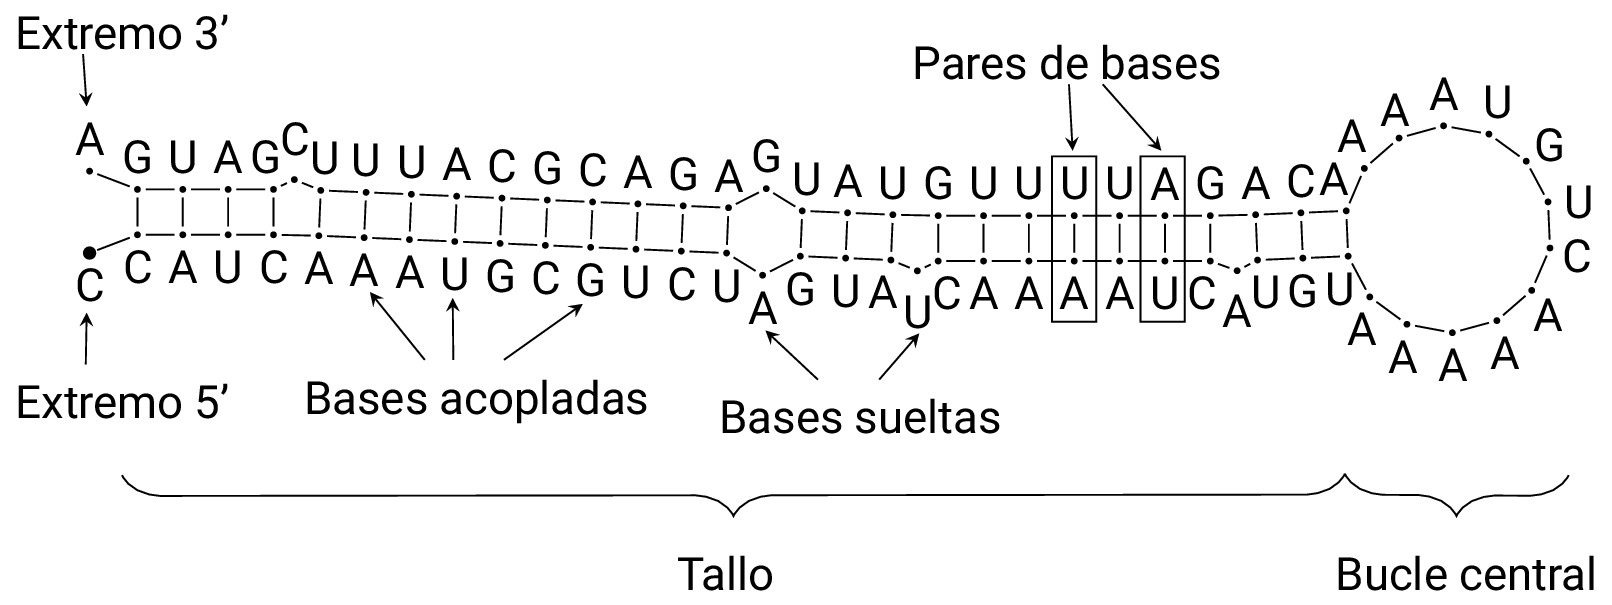
\includegraphics[width=.8\textwidth]{figures/hairpin_cel-lsy-6/hairpin.pdf}
%nnodes = 85
\shorthandoff{<}
\shorthandoff{>}
\tikzsetnextfilename{figures/hairpin_cel-lsy-6/hairpin}
\begin{tikzpicture}[scale=0.025,rotate=90,font=\small\sffamily,every label/.style={label distance=0}]
\tikzstyle{lstyle}=[shorten >= 2,shorten <= 2];
\coordinate[label={[xshift=0,yshift=0]below:C}] (1) at (93.0263,323.2249);
\fill[] (1) circle (2.2);
\coordinate[label={[xshift=0,yshift=0]below:C}] (2) at (99.0726,307.3858);
\fill[] (2) circle (1.1);
\coordinate[label={[xshift=0,yshift=0]below:A}] (3) at (99.0726,292.3858);
\fill[] (3) circle (1.1);
\coordinate[label={[xshift=0,yshift=0]below:U}] (4) at (99.0726,277.3858);
\fill[] (4) circle (1.1);
\coordinate[label={[xshift=0,yshift=0]below:C}] (5) at (99.0726,262.3858);
\fill[] (5) circle (1.1);
\coordinate[label={[xshift=0,yshift=0]below:A}] (6) at (98.7542,247.3892);
\fill[] (6) circle (1.1);
\coordinate[label={[xshift=0,yshift=0]below:A}] (7) at (98.1176,232.4027);
\fill[] (7) circle (1.1);
\coordinate[label={[xshift=0,yshift=0]below:A}] (8) at (97.4810,217.4162);
\fill[] (8) circle (1.1);
\coordinate[label={[xshift=0,yshift=0]below:U}] (9) at (96.8444,202.4297);
\fill[] (9) circle (1.1);
\coordinate[label={[xshift=0,yshift=0]below:G}] (10) at (96.2078,187.4432);
\fill[] (10) circle (1.1);
\coordinate[label={[xshift=0,yshift=0]below:C}] (11) at (95.5712,172.4568);
\fill[] (11) circle (1.1);
\coordinate[label={[xshift=0,yshift=0]below:G}] (12) at (94.9345,157.4703);
\fill[] (12) circle (1.1);
\coordinate[label={[xshift=0,yshift=0]below:U}] (13) at (94.2979,142.4838);
\fill[] (13) circle (1.1);
\coordinate[label={[xshift=0,yshift=0]below:C}] (14) at (93.6613,127.4973);
\fill[] (14) circle (1.1);
\coordinate[label={[xshift=0,yshift=0]below:U}] (15) at (93.0247,112.5108);
\fill[] (15) circle (1.1);
\coordinate[label={[xshift=0,yshift=0]below:A}] (16) at (85.6890,100.6079);
\fill[] (16) circle (1.1);
\coordinate[label={[xshift=0,yshift=0]below:G}] (17) at (91.9888,88.1258);
\fill[] (17) circle (1.1);
\coordinate[label={[xshift=0,yshift=0]below:U}] (18) at (91.3522,73.1393);
\fill[] (18) circle (1.1);
\coordinate[label={[xshift=-2,yshift=0]below:A}] (19) at (90.7156,58.1528);
\fill[] (19) circle (1.1);
\coordinate[label={[xshift=0,yshift=-2]below:U}] (20) at (87.1365,49.4132);
\fill[] (20) circle (1.1);
\coordinate[label={[xshift=2,yshift=0]below:C}] (21) at (90.3837,42.5196);
\fill[] (21) circle (1.1);
\coordinate[label={[xshift=0,yshift=0]below:A}] (22) at (90.3837,27.5196);
\fill[] (22) circle (1.1);
\coordinate[label={[xshift=2,yshift=0]below:A}] (23) at (90.3837,12.5196);
\fill[] (23) circle (1.1);
\coordinate[label={[xshift=0,yshift=0]below:A}] (24) at (90.3837,-2.4804);
\fill[] (24) circle (1.1);
\coordinate[label={[xshift=0,yshift=0]below:A}] (25) at (90.3837,-17.4804);
\fill[] (25) circle (1.1);
\coordinate[label={[xshift=0,yshift=0]below:U}] (26) at (90.3837,-32.4804);
\fill[] (26) circle (1.1);
\coordinate[label={[xshift=-2,yshift=0]below:C}] (27) at (90.3837,-47.4804);
\fill[] (27) circle (1.1);
\coordinate[label={[xshift=0,yshift=-2]below:A}] (28) at (87.1788,-56.3641);
\fill[] (28) circle (1.1);
\coordinate[label={[xshift=2,yshift=0]below:U}] (29) at (90.7156,-63.1136);
\fill[] (29) circle (1.1);
\coordinate[label={[xshift=0,yshift=0]below:G}] (30) at (91.3522,-78.1001);
\fill[] (30) circle (1.1);
\coordinate[label={[xshift=-2,yshift=0]below:U}] (31) at (91.9888,-93.0866);
\fill[] (31) circle (1.1);
\coordinate[label={[xshift=-2,yshift=0]below:A}] (32) at (78.5065,-100.2412);
\fill[] (32) circle (1.1);
\coordinate[label={[xshift=-1,yshift=0]below:A}] (33) at (69.4705,-112.5422);
\fill[] (33) circle (1.1);
\coordinate[label={[xshift=0,yshift=0]below:A}] (34) at (66.6749,-127.5471);
\fill[] (34) circle (1.1);
\coordinate[label={[xshift=2,yshift=0]below:A}] (35) at (70.6749,-142.2768);
\fill[] (35) circle (1.1);
\coordinate[label={[xshift=4,yshift=2]below:A}] (36) at (80.6762,-153.8066);
\fill[] (36) circle (1.1);
\coordinate[label={[xshift=-1,yshift=-2]right:C}] (37) at (94.6931,-159.8473);
\fill[] (37) circle (1.1);
\coordinate[label={[xshift=0,yshift=0]right:U}] (38) at (109.9425,-159.1995);
\fill[] (38) circle (1.1);
\coordinate[label={[xshift=-2,yshift=4]right:G}] (39) at (123.3966,-151.9918);
\fill[] (39) circle (1.1);
\coordinate[label={[xshift=2,yshift=0]above:U}] (40) at (132.3840,-139.6554);
\fill[] (40) circle (1.1);
\coordinate[label={[xshift=0,yshift=0]above:A}] (41) at (135.1205,-124.6396);
\fill[] (41) circle (1.1);
\coordinate[label={[xshift=0,yshift=0]above:A}] (42) at (131.0625,-109.9258);
\fill[] (42) circle (1.1);
\coordinate[label={[xshift=0,yshift=0]above:A}] (43) at (121.0159,-98.4354);
\fill[] (43) circle (1.1);
\coordinate[label={[xshift=0,yshift=0]above:A}] (44) at (106.9753,-92.4500);
\fill[] (44) circle (1.1);
\coordinate[label={[xshift=0,yshift=0]above:C}] (45) at (106.3387,-77.4635);
\fill[] (45) circle (1.1);
\coordinate[label={[xshift=0,yshift=0]above:A}] (46) at (105.7021,-62.4770);
\fill[] (46) circle (1.1);
\coordinate[label={[xshift=0,yshift=0]above:G}] (47) at (105.3837,-47.4804);
\fill[] (47) circle (1.1);
\coordinate[label={[xshift=0,yshift=0]above:A}] (48) at (105.3837,-32.4804);
\fill[] (48) circle (1.1);
\coordinate[label={[xshift=0,yshift=0]above:U}] (49) at (105.3837,-17.4804);
\fill[] (49) circle (1.1);
\coordinate[label={[xshift=0,yshift=0]above:U}] (50) at (105.3837,-2.4804);
\fill[] (50) circle (1.1);
\coordinate[label={[xshift=0,yshift=0]above:U}] (51) at (105.3837,12.5196);
\fill[] (51) circle (1.1);
\coordinate[label={[xshift=0,yshift=0]above:U}] (52) at (105.3837,27.5196);
\fill[] (52) circle (1.1);
\coordinate[label={[xshift=0,yshift=0]above:G}] (53) at (105.3837,42.5196);
\fill[] (53) circle (1.1);
\coordinate[label={[xshift=0,yshift=0]above:U}] (54) at (105.7021,57.5162);
\fill[] (54) circle (1.1);
\coordinate[label={[xshift=0,yshift=0]above:A}] (55) at (106.3387,72.5027);
\fill[] (55) circle (1.1);
\coordinate[label={[xshift=0,yshift=0]above:U}] (56) at (106.9753,87.4892);
\fill[] (56) circle (1.1);
\coordinate[label={[xshift=0,yshift=0]above:G}] (57) at (114.3110,99.3921);
\fill[] (57) circle (1.1);
\coordinate[label={[xshift=0,yshift=0]above:A}] (58) at (108.0112,111.8742);
\fill[] (58) circle (1.1);
\coordinate[label={[xshift=0,yshift=0]above:G}] (59) at (108.6478,126.8607);
\fill[] (59) circle (1.1);
\coordinate[label={[xshift=0,yshift=0]above:A}] (60) at (109.2844,141.8472);
\fill[] (60) circle (1.1);
\coordinate[label={[xshift=0,yshift=0]above:C}] (61) at (109.9210,156.8336);
\fill[] (61) circle (1.1);
\coordinate[label={[xshift=0,yshift=0]above:G}] (62) at (110.5576,171.8201);
\fill[] (62) circle (1.1);
\coordinate[label={[xshift=0,yshift=0]above:C}] (63) at (111.1943,186.8066);
\fill[] (63) circle (1.1);
\coordinate[label={[xshift=0,yshift=0]above:A}] (64) at (111.8309,201.7931);
\fill[] (64) circle (1.1);
\coordinate[label={[xshift=0,yshift=0]above:U}] (65) at (112.4675,216.7796);
\fill[] (65) circle (1.1);
\coordinate[label={[xshift=0,yshift=0]above:U}] (66) at (113.1041,231.7661);
\fill[] (66) circle (1.1);
\coordinate[label={[xshift=0,yshift=0]above:U}] (67) at (113.7407,246.7525);
\fill[] (67) circle (1.1);
\coordinate[label={[xshift=0,yshift=0]above:C}] (68) at (117.3198,255.4922);
\fill[] (68) circle (1.1);
\coordinate[label={[xshift=0,yshift=0]above:G}] (69) at (114.0726,262.3858);
\fill[] (69) circle (1.1);
\coordinate[label={[xshift=0,yshift=0]above:A}] (70) at (114.0726,277.3858);
\fill[] (70) circle (1.1);
\coordinate[label={[xshift=0,yshift=0]above:U}] (71) at (114.0726,292.3858);
\fill[] (71) circle (1.1);
\coordinate[label={[xshift=0,yshift=0]above:G}] (72) at (114.0726,307.3858);
\fill[] (72) circle (1.1);
\coordinate[label={[xshift=0,yshift=0]above:A}] (73) at (120.1190,323.2249);
\fill[] (73) circle (1.1);
\draw[lstyle] (1) -- (2);
\draw[lstyle] (2) -- (3);
\draw[lstyle] (3) -- (4);
\draw[lstyle] (4) -- (5);
\draw[lstyle] (5) -- (6);
\draw[lstyle] (6) -- (7);
\draw[lstyle] (7) -- (8);
\draw[lstyle] (8) -- (9);
\draw[lstyle] (9) -- (10);
\draw[lstyle] (10) -- (11);
\draw[lstyle] (11) -- (12);
\draw[lstyle] (12) -- (13);
\draw[lstyle] (13) -- (14);
\draw[lstyle] (14) -- (15);
\draw[lstyle] (15) -- (16);
\draw[lstyle] (16) -- (17);
\draw[lstyle] (17) -- (18);
\draw[lstyle] (18) -- (19);
\draw[lstyle] (19) -- (20);
\draw[lstyle] (20) -- (21);
\draw[lstyle] (21) -- (22);
\draw[lstyle] (22) -- (23);
\draw[lstyle] (23) -- (24);
\draw[lstyle] (24) -- (25);
\draw[lstyle] (25) -- (26);
\draw[lstyle] (26) -- (27);
\draw[lstyle] (27) -- (28);
\draw[lstyle] (28) -- (29);
\draw[lstyle] (29) -- (30);
\draw[lstyle] (30) -- (31);
\draw[lstyle] (31) -- (32);
\draw[lstyle] (32) -- (33);
\draw[lstyle] (33) -- (34);
\draw[lstyle] (34) -- (35);
\draw[lstyle] (35) -- (36);
\draw[lstyle] (36) -- (37);
\draw[lstyle] (37) -- (38);
\draw[lstyle] (38) -- (39);
\draw[lstyle] (39) -- (40);
\draw[lstyle] (40) -- (41);
\draw[lstyle] (41) -- (42);
\draw[lstyle] (42) -- (43);
\draw[lstyle] (43) -- (44);
\draw[lstyle] (44) -- (45);
\draw[lstyle] (45) -- (46);
\draw[lstyle] (46) -- (47);
\draw[lstyle] (47) -- (48);
\draw[lstyle] (48) -- (49);
\draw[lstyle] (49) -- (50);
\draw[lstyle] (50) -- (51);
\draw[lstyle] (51) -- (52);
\draw[lstyle] (52) -- (53);
\draw[lstyle] (53) -- (54);
\draw[lstyle] (54) -- (55);
\draw[lstyle] (55) -- (56);
\draw[lstyle] (56) -- (57);
\draw[lstyle] (57) -- (58);
\draw[lstyle] (58) -- (59);
\draw[lstyle] (59) -- (60);
\draw[lstyle] (60) -- (61);
\draw[lstyle] (61) -- (62);
\draw[lstyle] (62) -- (63);
\draw[lstyle] (63) -- (64);
\draw[lstyle] (64) -- (65);
\draw[lstyle] (65) -- (66);
\draw[lstyle] (66) -- (67);
\draw[lstyle] (67) -- (68);
\draw[lstyle] (68) -- (69);
\draw[lstyle] (69) -- (70);
\draw[lstyle] (70) -- (71);
\draw[lstyle] (71) -- (72);
\draw[lstyle] (72) -- (73);
\draw[lstyle] (2) -- (72);
\draw[lstyle] (3) -- (71);
\draw[lstyle] (4) -- (70);
\draw[lstyle] (5) -- (69);
\draw[lstyle] (6) -- (67);
\draw[lstyle] (7) -- (66);
\draw[lstyle] (8) -- (65);
\draw[lstyle] (9) -- (64);
\draw[lstyle] (10) -- (63);
\draw[lstyle] (11) -- (62);
\draw[lstyle] (12) -- (61);
\draw[lstyle] (13) -- (60);
\draw[lstyle] (14) -- (59);
\draw[lstyle] (15) -- (58);
\draw[lstyle] (17) -- (56);
\draw[lstyle] (18) -- (55);
\draw[lstyle] (19) -- (54);
\draw[lstyle] (21) -- (53);
\draw[lstyle] (22) -- (52);
\draw[lstyle] (23) -- (51);
\draw[lstyle] (24) -- (50);
\draw[lstyle] (25) -- (49);
\draw[lstyle] (26) -- (48);
\draw[lstyle] (27) -- (47);
\draw[lstyle] (29) -- (46);
\draw[lstyle] (30) -- (45);
\draw[lstyle] (31) -- (44);

%%%%%%%%%%%%%%%%

\usetikzlibrary{decorations.pathreplacing};
\coordinate (stemloop) at (20,-92);
\draw[decorate,decoration={brace, amplitude=10}] (stemloop)
to node [midway, label={[label distance=-20,below]:Tallo}] {} (20,320);
\draw[decorate,decoration={brace, amplitude=10}] (20,-170)
to node [midway, label={[label distance=-20,below]:Bucle central}] {} (stemloop);

\node (loose) at (40,70) {Bases sueltas};
\node (paired) at (45,200) {Bases acopladas};
\draw[-stealth] (loose) -- (70,50);
\draw[-stealth] (loose) -- (70,100);
\draw[-stealth] (paired) -- (80,160);
\draw[-stealth] (paired) -- (82,200);
\draw[-stealth] (paired) -- (84,230);

\draw[dotted] (73,-10) rectangle (125,6);
\draw[dotted] (73,-40) rectangle (125,-24);
\node (par) at (160,00) {Pares de bases};
\draw[-stealth] (par) -- (130,-2);
\draw[-stealth] (par) -- (130,-32);

\node (e5) at (45,320) {Extremo 5'};
\node (e3) at (170,320) {Extremo 3'};
\draw[-stealth] (e5) -- (75,330);
\draw[-stealth] (e3) -- (145,330);


\end{tikzpicture}
\shorthandon{<}
\shorthandon{>}


\caption{\captionStyle\protect\label{fig:hairpin-parts} Nomenclatura de las diferentes partes que
componen una la estructura secundaria típica en forma de horquilla.
El ejemplo corresponde a \protect\dset{lsy-6}, un \premirna{} de la
especie \e{C. elegans}, extraído de \work\mirbase{} versión 21.
}
\end{figure}
%
% esta footnote corresponde a la figura hairpin
\footnotetext{Fuente: \url{http://mirbase.org/cgi-bin/mirna_entry.pl?acc=MI0000801}.}
%
%
%
\subsubsection{Características de tripletes}
%
Las \caract{s} de tripletes, propuestas en el método \work{Triplet-SVM}
\cite{xue}, se basan en la idea de que la propiedad distintiva de los
\premirna{s} es una estructura secundaria en forma de horquilla
con una alta complementariedad entre las bases que forman el \e{tallo}.
%% En el trabajo original, los autores proponen un método para clasificar
%% secuencias con estructura secundaria en forma de horquilla entrenando
%% con \premirna{s} ``reales'' y otras secuencias con la misma estructura
%% secundaria denominadas ``pseudo \premirna{s}''.
Esta idea surge a partir de observar que la distribución
(frecuencia de aparición) de unas sub-estructuras locales llamadas
``tripletes'' difiere significativamente entre los ejemplos que
representan \premirna{s} y los ejemplos de otro tipo.

%% A partir de estas observaciones, proponen generar un conjunto de
%% \caract{s} que representa la distribución de las sub-estructuras
%% locales dentro del ``tallo'' de la horquilla.

Un ``triplete'' es una cadena de caracteres que relaciona la base de
un nucleótido (\ntA{}, \ntC{}, \ntG{}, o \ntU{}) en la posición $i$ con su
estructura secundaria local en $i-1,i,i+1$, representada en forma
binaria como ``acoplado'' \pairL{} (paréntesis) y ``no acoplado''
\noPair{} (punto).
El conjunto de \caract{s} de tripletes incluye medidas que cuentan
el número de ocurrencias de las $32$ combinaciones de tripletes posibles
($4$ bases $\cdot$ $2^3$ combinaciones de estado)
en la región del tallo, junto con $4$ medidas auxiliares que surgen
de cálculos intermedios:
%
\begin{itemize}
\item longitud del tallo $L_3$,
\item número de pares de bases $P$,
\item complementariedad de ambos brazos de la horquilla,
\item proporción de bases \ntG{} y \ntC{} en la zona del tallo.
\end{itemize}
%
En la \iflatexml{}Figura~\ref{triplet}\else\autoref{triplet}\fi{} se
representa en forma gráfica el proceso de extracción de las \caract{s}
de tripletes.

\begin{figure}[H]
\figureStyle
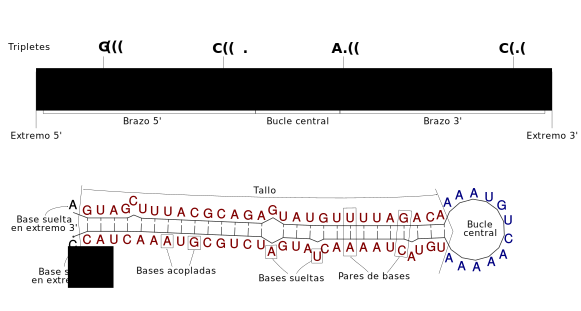
\includegraphics[width=\textwidth]{figures/triplet/triplete.pdf}

\caption{\captionStyle\protect\label{triplet}
Ejemplo de extracción de características de tripletes para el
\premirna{} \dset{cel-lsy-6}.
}
\end{figure}
%
%
\subsubsection{Características de tripletes}
%
Las \caract{s} de tripletes, propuestas en el método \work{Triplet-SVM}
\cite{xue}, se basan en la idea de que la propiedad distintiva de los
\premirna{s} es una estructura secundaria en forma de horquilla con
una alta complementariedad entre sus ``brazos''.
%% En el trabajo original, los autores proponen un método para clasificar
%% secuencias con estructura secundaria en forma de horquilla entrenando
%% con \premirna{s} ``reales'' y otras secuencias con la misma estructura
%% secundaria denominadas ``pseudo \premirna{s}''.
Las \caract{s} de tripletes se justifican en la observación empírica
que la distribución (frecuencia de aparición) de sub-estructuras
locales en la región del tallo de la horquilla difiere
significativamente entre los \premirna{s} ``reales'' y los ejemplos de
clase negativa, que también poseen estructura secundaria en forma de
horquilla.

%% A partir de estas observaciones, proponen generar un conjunto de
%% \caract{s} que representa la distribución de las sub-estructuras
%% locales dentro del ``tallo'' de la horquilla.

Un ``triplete'' es una cadena de caracteres que relaciona la base de
un nucleótido en la posición $i$ (\ntA, \ntC, \ntG, o \ntU) con su
estructura secundaria local en $i-1,i,i+1$, representada en forma
binaria como ``acoplado'' \pairL (paréntesis) y ``no acoplado''
\noPair (punto).
El conjunto de \caract{s} de tripletes incluye medidas que cuentan
el número de ocurrencias de las 32 combinaciones posibles de tripletes
en la región del tallo, junto con 4 medidas auxiliares derivadas
del cálculo de los tripletes:
%
\begin{itemize}
\item longitud del tallo,
\item número de pares de bases,
\item complementariedad de ambos brazos de la horquilla,
\item proporción de bases \ntG y \ntC en la zona del tallo.
\end{itemize}
%

En la \iflatexml{}Figura~\ref{triplet}\else\autoref{triplet}\fi{} se
ilustra el proceso de extracción de tripletes para el \premirna{}
\sbs{cel-lsy-66} correspondiente al organismo modelo \e{C. elegans}
\cite{mirbase1}, con anotaciones que indican las distintas partes que
componen la horquilla: tallo, bucle central, brazos, extremos, bases
sueltas y acopladas, y pares de bases.

La principal limitación de las características de tripletes reside en
que su cálculo resulta posible únicamente cuando la estructura
secundaria tiene forma de horquilla, ya que de otro modo la definición
del ``tallo'' pierde sentido. Por ello, estas \caract{s} no se
calculan cuando el ejemplo contiene bucles múltiples en su estrucutra
secundaria.

En la tabla a continuación se detallan las 36 características de
tripletes y su posición en el vector de características.

\newcommand{\tripletRow}[1]{
  \stepcounter{FeatureCounter}\theFeatureCounter &
  \dset{T} & $N_{\T{\mono{#1}}}$ &
  Número de ocurrencias del triplete \mono{#1} en la región del
  tallo. \iflatexml{}\\\fi
  }

\begin{longtable}{@{}p{0.07\textwidth}%
@{\hspace{0.01\textwidth}}p{0.07\textwidth}%
@{\hspace{0.01\textwidth}}p{0.13\textwidth}%
@{\hspace{0.01\textwidth}}p{0.70\textwidth}@{}}
  \headRow\endhead\iflatexml{}\\\fi
  \tripletRow{A...}\\
  \tripletRow{A..(}\\
  \tripletRow{A.(.}\\
  \tripletRow{A.((}\\
  \tripletRow{A(..}\\
  \tripletRow{A(.(}\\
  \tripletRow{A((.}\\
  \tripletRow{A(((}\\
  \tripletRow{G...}\\
  \tripletRow{G..(}\\
  \tripletRow{G.(.}\\
  \tripletRow{G.((}\\
  \tripletRow{G(..}\\
  \tripletRow{G(.(}\\
  \tripletRow{G((.}\\
  \tripletRow{G(((}\\
  \tripletRow{C...}\\
  \tripletRow{C..(}\\
  \tripletRow{C.(.}\\
  \tripletRow{C.((}\\
  \tripletRow{C(..}\\
  \tripletRow{C(.(}\\
  \tripletRow{C((.}\\
  \tripletRow{C(((}\\
  \tripletRow{U...}\\
  \tripletRow{U..(}\\
  \tripletRow{U.(.}\\
  \tripletRow{U.((}\\
  \tripletRow{U(..}\\
  \tripletRow{U(.(}\\
  \tripletRow{U((.}\\
  \tripletRow{U(((}\\
  33 & \dset{X} & $L_3$ &
  Longitud del tallo: cantidad de nucleótidos en el tallo de
  la estructura de horquilla. \\
  34 & \dset{X} & $P$ &
  Número de pares de bases en el \premirna{}. \\
  35 & \dset{X} & $L_3/P$ &
  Grado de complementariedad entre los dos brazos de la estructura de
  horquilla: para una complementariedad perfecta, se da el valor
  mínimo 2. Este valor aumenta conforme aumenta el número de
  bases ``sueltas'' (no acopladas) en el tallo. \\
  36 & \dset{X} & $GC=\frac{N_\ntC{}+N_\ntG{}}{L_3}$ &
  Proporción de bases \ntG{} y \ntC{} en el tallo.  Se calcula contando el
  número de bases \ntC{} y \ntG{} en el tallo y dividiendo por $L_3$.
\end{longtable}

%
%
\subsubsection{Características de la secuencia}
%
Las \caract{s} de la secuencia se proponen en los trabajos \e{miPred}
\cite{ng} y \e{microPred} \cite{batuwita}.
Estas \caract{s} se calculan directamente a partir de la secuencia,
ignorando las propiedades de la estructura secundaria.
Se incluyen medidas que cuentan la longitud de la secuencia, el número
de ocurrencias de las bases \ntA, \ntG, \ntC y\ntU en forma individual
y en combinaciones de dos posiciones consecutivas (dinucleótidos).
En la tabla a continuación se enumeran las 23 \caract{s} de la
secuencia según la posición que ocupan en el vector de \caract{s}.

\newcommand{\dnRow}[1]{
  \stepcounter{FeatureCounter}\theFeatureCounter
  & $N_{\T{\mono{#1}}}$
  & Número de dinucleótidos \mono{#1}.}
%
\setcounter{FeatureCounter}{43}
%
\begin{longtable}{@{}p{0.07\textwidth}%
@{\hspace{0.01\textwidth}}p{0.13\textwidth}%
@{\hspace{0.01\textwidth}}p{0.78\textwidth}@{}}
  \headRow\endhead
  37 & $L$ &
  Longitud de la secuencia. \\
  38 & $N_\ntA{}$ &
  Número de nucleótidos \ntA{}. \\
  39 & $N_\ntC{}$ &
  Número de nucleótidos \ntC{}. \\
  40 & $N_\ntG{}$ &
  Número de nucleótidos \ntG{}. \\
  41 & $N_\ntU{}$ &
  Número de nucleótidos \ntU{}. \\
  42 & $N_\ntC{}+N_\ntG{}$ &
  Número de nucleótidos \ntC{} y \ntG{}. \\
  43 & $N_\ntA{}+N_\ntU{}$ &
  Número de nucleótidos \ntA{} y \ntU{}. \\
  \dnRow{AA}\\
  \dnRow{AC}\\
  \dnRow{AG}\\
  \dnRow{AU}\\
  \dnRow{CA}\\
  \dnRow{CC}\\
  \dnRow{CG}\\
  \dnRow{CU}\\
  \dnRow{GA}\\
  \dnRow{GC}\\
  \dnRow{GG}\\
  \dnRow{GU}\\
  \dnRow{UA}\\
  \dnRow{UC}\\
  \dnRow{UG}\\
  \dnRow{UU}\\
\end{longtable}

%
%
\subsubsection{Características de la estructura secundaria}
%
Este grupo de \caract{s} incluye medidas relacionadas con la
estructura secundaria, tales como la ocurrencia de diferentes tipos de
pares de bases (bases acopladas) \bp{A}{U}, \bp{G}{C}, y \bp{G}{U}, así
como medidas basadas en la \e{Mínima Energía Libre}, un valor
resultante del algoritmo de plegado (predicción de la estructura
secundaria).  Al igual que las medidas de la secuencia, este grupo
de \caract{s} se basa en aquellas utilizadas en \cite{ng}
y \cite{batuwita}.  A continuación se detallan las 7 \caract{s} que
componen este grupo y su posición dentro del vector global
de \caract{s}.

\begin{longtable}{@{}p{0.07\textwidth}%
@{\hspace{0.01\textwidth}}p{0.07\textwidth}%
@{\hspace{0.01\textwidth}}p{0.13\textwidth}%
@{\hspace{0.01\textwidth}}p{0.70\textwidth}@{}}
  \headRow\endhead
  60 & \dset{E} & MFE &
  Mínima energía libre. \\
  61 & \dset{E} & MFEI$_1$ &
  MFEI$_1=\frac{\T{MFE}}{100\cdot(N_\ntC{}+N_\ntG{})}$. \\
  62 & \dset{E} & MFEI$_4$ &
  MFEI$_4=\T{MFE}/P$. \\
  63 & \dset{E} & $dP = P/L$ &
  Número de pares de bases dividido entre la longitud total $L$. \\
  64 & \dset{E} & $P_{\bp{A}{U}}/L$ &
  Número de pares \bp{A}{U} normalizado. \\
  65 & \dset{E} & $P_{\bp{G}{C}}/L$ &
  Número de pares \bp{G}{C} normalizado. \\
  66 & \dset{E} & $P_{\bp{G}{U}}/L$ &
  Número de pares \bp{G}{U} normalizado.
\end{longtable}

%
%
%
\subsection{Normalización de los vectores de características}
%
Las \caract{s} que componen el vector de \caract{s} poseen rangos
numéricos diferentes, ya que representan cantidades de naturaleza
diversa.
Esto implica que algunos componentes del vector de \caract{s} tendrán
magnitudes mayores que otros, generando una ponderación implícita de
algunas \caract{s} por sobre otras.
La normalización permite evitar este problema modificando el rango de
cada \caract{} a un intervalo preestablecido, típicamente $[0,1]$ o
$[-1,+1]$.
Esto deriva en problemas mejor condicionados desde el punto de vista
numérico e incrementa la velocidad de convergencia en el
entrenamiento \cite{nnfaq2}.

Dado un vector de características $\xx=(x_{1},x_{2},\ldots,x_{F})$, la
versión normalizada $\xx^*$ del mismo vector se calcula según
%
\begin{align}
  \label{e3:norm-op}
  x_j^{*} = ( x_j + d_j ) s_j, \quad j=1,\ldots,F,
\end{align}
%
donde $\B{s}$ es un \e{vector de escala} y $\B{d}$ es un \e{vector de
  desplazamiento} que permiten transformar las componentes $x_j$ al
intervalo especificado.

Cuando el objetivo es la generación de un modelo de clasificador, los
vectores $\B{s}$ y $\B{d}$ se calculan con el primer archivo leído a
la entrada del método.
El primer paso es armar una matriz
$M{}_{({N}\times{}F)}$, donde cada fila $i=1,\ldots,N$ corresponde a
un ejemplo y cada columna $j=1,\ldots,F$ representa una variable
(\caract{}).
Para cada columna $j$ de $M$, se calculan los valores $d_j$ y $s_j$
que transforman el rango de la variable $x_j$ al intervalo deseado.
Para llevar las variables al rango $[0,1]$, $d_j$ y $s_j$ se
calculan según
%
\begin{align}
  d_j &= - \min_i m_{ij}, &
  s_j &= \frac{1}{\max_i m_{ij} - \min_i m_{ij}}.
\end{align}
%
Similarmente, para llevar las variables al intervalo simétrico
$[-1,+1]$,
%
\begin{align}
  d_j &= -\frac{1}{2}\left(\max_i m_{ij} + \min_i m_{ij}\right), &
  s_j &= \frac{2}{\max_i m_{ij} - \min_i m_{ij}}.
\end{align}
%
Una vez calculados los vectores $\B{d}$ y $\B{s}$, se aplica la
normalización (\iflatexml{}Ecuación~\ref{e3:norm-op}\else\autoref{e3:norm-op}\fi)
sobre todos los ejemplos leídos en la entrada.

Para un modelo de clasificador entrenado con datos normalizados, es
importante aplicar la misma normalización sobre todos los ejemplos
futuros a clasificar.
Por ello, los vectores $\B{d}$ y $\B{s}$ se guardan como parte del
mismo modelo.
Cuando se provee un modelo como entrada al método, los ejemplos se
normalizan según la información contenida en el mismo.

%
%
%
\subsection{Particionado de los datos}
%
El particionado separa los datos leídos en conjuntos de entrenamiento,
utilizado para la generación del modelo del clasificador, y de prueba,
que contiene los ejemplos a usar para clasificación.
La composición de estos conjuntos viene determinada por la
especificación del usuario, que debe indicar, para cada archivo, el
número de elementos a utilizar para entrenamiento y para prueba.
Cuando el archivo se utiliza para entrenamiento, se debe indicar
adicionalmente la clase de los ejemplos que contiene.

El primer paso es ``etiquetar'' los vectores normalizados, extendiéndolos
con números de referencia que indican el archivo de origen, la
posición del dato original dentro del archivo, y la clase del ejemplo
en cuestión.
El segundo paso armar los conjuntos de entrenamiento y prueba como
matrices, cuyas filas son vectores ``etiquetados'' seleccionados al
azar de cada archivo, respetando las proporciones indicadas por el
usuario.
Una vez incorporados todos los ejemplos a los conjuntos de
entrenamiento y prueba, se permutan las filas de ambas matrices en
forma pseudoaleatoria.

La partición de los datos se efectúa de forma tal que los conjuntos de
entrenamiento y prueba resultantes sean disjuntos: si un ejemplo se
incorpora al conjunto de prueba, no será parte del conjunto de
entrenamiento, y viceversa.

%% %
%% \subsubsection{Sobremuestreo de la clase minoritaria}
%% %
%% El método permite efectuar sobremuestreo de la clase minoritaria en el
%% conjunto de entrenamiento, repitiendo ejemplos seleccionados
%% aleatoriamente hasta igualar en número a los ejemplos de la clase
%% mayoritaria.
%% Esto resulta útil para entrenar clasificadores sensibles al desbalance
%% de clases, tales como el perceptrón multicapa, evitando que el modelo
%% resultante presente un sesgo hacia la clase mayoritaria.
\pdfmargincomment[icon=note]{Saco la seccion de
  sobremuestreo directamente, ya que no aporta nada: tampoco hice
  pruebas en el Cap4.}

%
%
\subsubsection{Generación de particiones para validación cruzada}
%
%La generación de las particiones de validación cruzada se lleva a cabo
%una vez armado el conjunto de entrenamiento con $\ell^E$ elementos.
Las particiones de validación cruzada se generan como un conjunto de
índices sobre el conjunto de entrenamiento.
En primer lugar, se genera un vector de índices en orden aleatorio
entre $1$ y $\ell^E$, el número de ejemplos en el conjunto de
entrenamiento.
Luego se seleccionan los primeros $p\cdot\ell^E$ elementos para la
partición de validación, y los elementos restantes para la partición
de estimación correspondiente.
La operación se repite para cada $j=1,\ldots,k$, efectuando un
desplazamiento circular del vector de índices en $\ell^E/k$ elementos
entre iteraciones.
El parámetro $p$ regula la proporción de elementos de entrenamiento a
utilizar para validación, mientras que $k$ determina el número de
iteraciones de la validación cruzada.
Ambos parámetros pueden ser especificados por el usuario, y por
defecto se utilizan los valores $k=10$ $p=1/$.
Cuando $p=1/k$, cada ejemplo del conjunto de entrenamiento será
utilizado exactamente una vez para validación.

%
%
%
\section{Construcción del modelo del clasificador MLP}
%
El primer paso para la construcción de un modelo MLP es determinar el
número óptimo de neuronas en la capa oculta mediante una estrategia
de búsqueda exhaustiva que maximiza la tasa \GM{} promedio de
validación cruzada.
%% Para ello, se utiliza una estrategia de prueba y error, que prueba
%% distintos modelos mediante validación cruzada, y selecciona como
%% número óptimo de neuronas el de aquel modelo que obtiene la mejor tasa
%% $G_m$ en promedio sobre el conjunto de validación.
Alternativamente, se define una estrategia de selección trivial que
siempre selecciona 0 neuronas en la capa oculta, resultando en un
clasificador lineal.

Una vez determinado el número óptimo de neuronas en la capa oculta,
se procede al entrenamiento del modelo final utilizando el conjunto
de entrenamiento completo.

%% uego se procede a efectuar el entrenamiento propiamente dicho, con
%% regularización de corte prematuro cuando el error de validación
%% cruzada alcanza su valor mínimo.

%% La arquitectura de la red resultante contendrá una o ninguna capa
%% oculta.

%% En todo entrenamiento del clasificador, se promedian en realidad cinco
%% redes inicializadas aleatoriamente, y la salida del clasificador en
%% realidad es un voto mayoritario de la salida de estas cinco redes.

%% Adicionalmente, se acepta el valor especial de 0 neuronas ocultas para
%% representar un MLP sin capa oculta, capaz de efectuar clasificación lineal.

%% Las estrategias de selección del \hparam{} de la red (el número de
%% neuronas en la capa oculta) son
%% %
%% \begin{description}
%% \item[Estrategia trivial:] Consiste en seleccionar cero neuronas
%%   en la capa oculta, sin entrenamiento. Esto redunda en una red que es
%%   capaz de efectuar separación lineal, y se utiliza como criterio de base para
%%   establecer el rendimiento de la red.
%% \item[Estrategia de búsqueda exhausiva:] Consiste en determinar, mediante prueba y error,
%%   el número óptimo de neuronas que maximizan una tasa promedio de validación cruzada.
%% \end{description}
%% %
%% Una vez encontrado el valor óptimo, se procede al entrenamiento.

%
\subsection{Estrategia trivial}
%
La estrategia trivial retorna siempre el valor 0 como cantidad
``óptima'' de neuronas en la capa oculta, ignorando los datos de
entrenamiento.
El modelo de clasificador MLP resultante del entrenamiento siempre
equivale a un perceptrón simple, que funciona como un clasificador
lineal.
Si bien resulta claro que esta estrategia no efectssss ningnnnn tipo
de optimización, su utilidad reside en que el modelo resultante puede
tomarse como base en la comparación de distintos modelos MLP para el
problema dado.
%
%% En el caso de las
%% máquinas de vectores de soporte, la estrategia selecciona el valor $1$
%% para el hiperparámetro de regularización $C$ \cite{libsvm}, y un valor
%% $\gamma=\frac{1}{2F}$ para el hiperparámetro de amplitud del núcleo
%% RBF, donde $F$ es el número de características consideradas
%% \cite{glasmachersigel}.
%

%
\subsection{Búsqueda exhaustiva}
%
La estrategia de búsqueda exhaustiva determina el número óptimo de
neuronas ocultas mediante prueba y error, entrenando modelos con
diferentes cantidades de neuronas en la capa oculta y seleccionando
aquel que obtiene la mayor tasa \GM{} de validación cruzada en
promedio.

Dado que no existe una regla general para determinar el número
recomendado de neuronas ocultas \cite{nnfaq3}, se establece un rango
de prueba de entre 0 y 200.
Por razones de costo computacional, en lugar de efectuar la búsqueda
sobre todos los valores posibles, se prueban 20 valores $h$ entre 0 y
200 en una escala aproximadamente logarítmica:
%
\begin{align}
  \label{mlp-hidden-tries}
  h=0,1,2,3,4,5,7,9,11,14,19,24,32,41,54,70,91,118,154,200.
\end{align}
%
%% La estrategia genera selecciona aquel valor de $h$ para el cual se obtuvo
%% el mayor \GM de validación cruzada en promedio.

%
\subsubsection{Entrenamiento}
%
Una vez determinados los hiperparámetros óptimos del clasificador
mediante alguna de las estrategias descriptas previamente, se entrena
una máquina de aprendizaje (SVM o MLP) con el conjunto de
entrenamiento completo $D$, obteniendo un modelo ``final''.

La salida del método consiste en el modelo de la máquina de
aprendizaje correspondiente, el cual servirá, junto a una
especificación del escalado y offset a utilizar, para clasificar
elementos nuevos.

Para el caso del perceptrón multicapa, el modelo en realidad
consiste en 5 redes neuronales inicializadas con datos aleatorios
y entrenadas con el mismo conjunto de datos $D$.
De este modo, se neutraliza hasta cierto punto los efectos negativos
que una red mal ondicionada pudiera generar un mal modelo.

{\Huge \hl{Agregar detalles implementacion pertinentes}}

%
%
\section{Construcción del modelo del clasificador SVM}
%
Tal como en el caso del perceptrón multicapa, la construcción del
modelo SVM es un proceso de dos etapas: en primer lugar se determinan
valores óptimos para los \hparam{s}, y una vez encontrados, se procede
a entrenar el modelo final con los datos de entrenamiento y los
\hparam{s} óptimos encontrados.
%% A diferencia del caso MLP, sin embargo, en una máquina de vectores de
%% soporte puede haber más de un \hparam{}, y en general éstos se trata
%% de variables continuas.

Las propiedades analíticas de la SVM permiten aplicar estrategias de
selección de hiperparámetros más complejas que en el caso del MLP, que
en general resultan computacionalmente más eficientes.
Las cuatro estrategias de selección de \hparam{s} aplicables al
clasificador SVM son:
%
\begin{itemize}
\item
  Selección trivial: Retorna valores preestablecidos para los
  \hparam{s}, sin efectuar entrenamiento.
\item
  Búsqueda en la grilla: Efectúa una búsqueda exhaustiva de los
  hiperparámetros, maximizando la tasa de clasificación de validación
  cruzada.
\item
  Minimización del error empírico: Minimiza, mediante descenso por
  gradiente en el espacio de los \hparam{s}, una función que representa
  el error de clasificación de validación cruzada.
\item
  Minimización de la cota radio-margen: Minimiza mediante descenso por
  gradiente en el espacio de los \hparam{s} una función de derivación
  teórica que se relaciona con el error de clasificación.
\end{itemize}
%

%
%
\subsection{Selección trivial}
%
La estrategia de selección trivial consiste en seleccionar valores
preestablecidos (genéricos) para los hiperparámetros, apropiados para
la mayoría de los problemas.
El valor preestablecido para el hiperparámetro de regularización $C$
es $1$ \cite{libsvm}.
En el caso del hiperparámetro de amplitud del núcleo RBF, se calcula
un valor $\gamma=\frac{1}{2F}$, donde $F$ es el número de elementos en
el vector de características \cite{glasmachersigel}.

Es de esperar que el modelo resultante del uso de esta estrategia no
sea óptimo, aunque sí resulta de utilidad como base para la
comparación contra otros modelos parametrizados con estrategias más
complejas.

%
%
\subsection{Búsqueda en la grilla}
%
La \e{búsqueda en la grilla} es una estrategia heurística basada en el
método propuesto en \cite{hsu} que calcula valores óptimos para los
\hparam{s} de regularización $C$ y de amplitud del núcleo RBF
$\gamma$.
La estrategia considera las combinaciones de $(C,\gamma)$ como
``coordenadas en el espacio de los \hparam{s}''.
En cada punto $(C,\gamma)$, se entrena el clasificador con los
\hparam{s} correspondientes y se evalúa el resultado de validación
cruzada.
La búsqueda comienza con una ``grilla'' de puntos espaciados a
intervalos regulares y continúa interpolando en las cercanías de
aquellos puntos donde se obtuvo las mayores tasas de clasificación de
validación cruzada.

La grilla inicial viene dada por las coordenadas $C$-$\gamma$
%
\begin{align}
  \label{initial-grid}
  \log_2 C     \tab= -5, -3, -1, 1, \ldots, 15, \tabs
  \log_2\gamma \tab= -15,-13, -11, \ldots, 3.
\end{align}
%
Para cada punto $(C_i,\gamma_j)$, se entrena un modelo con los
\hparam{s} correspondientes y se clasifican las particiones de
validación cruzada, obteniendo una tasa $\GM_{ij}$ promedio.

La interpolación de la grilla se lleva a cabo mediante alguno de los
siguientes algoritmos heurísticos:
%
\begin{itemize}
\item
  \e{Zoom}: interpola una región centrada en el punto con mayor tasa
  de clasificación, reduciendo el área de búsqueda a $1/2$ de la
  amplitud anterior en cada dimensión.
\item
  \e{Umbral}: interpola puntos intermedios alrededor de las
  coordenadas cuyo resultado se ubica por encima de un valor
  ``umbral'', por defecto el percentil 90 de toda la grilla.
  Este algoritmo es el utilizado por defecto.
\item
  \e{$n$-mejores}: similar al umbral, interpola la grilla alrededor de
  los $n$ puntos con mejores resultados de validación cruzada.
\end{itemize}
%
Luego de efectuar la interpolación, se entrena y prueba el
clasificador sobre los nuevos puntos generados.
El procedimiento se repite $N$ iteraciones (por defecto, $N=3$).

La búsqueda en la grilla tiene la ventaja de ser conceptualmente
simple, sin embargo, no resulta escalable a más de dos dimensiones.
Dado que se trata de un método de búsqueda exhaustiva, resulta
comparativamente lento.
Cuando se trabaja con un clasificador SVM con núcleo lineal, se
establece la coordenada $\gamma=0$, y la grilla resultante tiene una
única dimensión, la del hiperparámetro $\log C$.

%
%
\subsection{Criterio del error empírico}
%
El \e{criterio del error empírico} es una estrategia que optimiza los
\hparam{s} del clasificador minimizando una función objetivo
denominada \e{error empírico}\,\footnote{
  El lector experto encontrará ambigua la denominación de la función
  ``error empírico'', ya que en la disciplina este nombre se utiliza
  como equivalente de ``error de entrenamiento''.
  En este trabajo, se mantiene la denominación de los autores
  \cite{ayat}, definiendo ``error empírico'' como la función que
  calcula un error probabilístico de validación cruzada sobre el
  conjunto de entrenamiento.
}, basada en la propuesta presentada en \cite{ayat}.
La función de error empírico mide el error de validación cruzada sobre
el conjunto de entrenamiento acoplando un modelo probabilístico a la
salida del clasificador, y permite su optimización mediante descenso
por gradiente ya que sus derivadas respecto de los \hparam{s} son
calculables.

En la propuesta original \cite{ayat}, la función {error empírico} se
optimiza únicamente respecto a los \hparam{s} del núcleo.
En la estrategia implementada, se agregó soporte para la optimización
del hiperparámetro $C$, siguiendo el método del cálculo de la derivada
respecto de $C$ propuesto en \cite{keerthi} y \cite{glasmachers}, tal
como se implementa en \cite{shark}.

%
\subsubsection{La función error empírico}
%
La función error empírico es la función objetivo a minimizar, y se
construye a partir de una estimación de la probabilidad de error del
modelo sobre el conjunto de entrenamiento.
Esta función posee características deseables de continuidad y
derivabilidad que permiten su optimización mediante descenso por
gradiente.

Considerando en primer lugar la pérdida $0-1$ promedio del modelo $h$
sobre un conjunto de validación $V=((\xx_k,y_k)),\,i=1,\ldots,\ell^V$,
se observa que este error puede escribirse
%
\begin{align}
\label{e3:error-test-alt}
E^V \tab = \frac{1}{\ell^V}\sum_{k=1}^{\ell^V} H(-{y}_k {h}(\xx_k))
\tabs = \frac{1}{\ell^V}\sum_{k=1}^{\ell^V} L_{0-1}(y_k,h(\xx_k)).
\end{align}
%
El uso de la función escalón unitario de Heaviside $H(\cdot)$ pone de
relieve el hecho que $E^V$ es una suma de funciones discontinuas, y
por lo tanto no es derivable.
Para salvar esta limitación, la función error empírico se construye a
partir de una estimación $\hat{p}_k$ de la \e{probabilidad a
  posteriori} $p_k$ de que el ejemplo $\xx_k$ pertenezca a la clase
positiva
%
\begin{align}
  \label{e3:pk}
  p_k = p(\xx_k) = P(h(\xx_k)=+1|\xx_k).
\end{align}
%
Por el momento, se supone que $p_k$ es una función continua y
derivable.
La \e{probabilidad de error} $E_k$ del modelo al clasificar el ejemplo
$\xx_k$ puede escribirse en términos de la probabilidad $p_k$ según
%
\begin{align}
\label{e3:Ek}
  E_k = P(h(\xx_k)\neq y_k) = |t_k-{p}_k| =
  \begin{cases}
    {p}_k, & t_k=0\\ 1-{p}_k, & t_k = 1,
  \end{cases}
\end{align}
%
en donde $t_k=\frac{1}{2}({y_k+1})$ es un ``valor deseado'' calculado
a partir de la clase conocida $y_k$.
El error empírico es simplemente la probabilidad de error promedio
para el conjunto completo $V$:
%
\begin{align}
\label{Err1}
  E = \frac{1}{\ell^V}\sum_{j=1}^{\ell^V} E_k.
\end{align}
%
Para el cálculo exacto de $E$ se requiere conocer la probabilidad
$p_k$ (\iflatexml{}Ecuación~\ref{e3:pk}\else\autoref{e3:pk}\fi), la
cual no puede determinarse a partir de la salida binaria del modelo
SVM.
En su lugar se utiliza un estimador $\hat{p}_k$, que se obtiene
ajustando un modelo probabilístico a la salida del modelo, tal como se
explica a continuación.

%
\subsubsection{Salida probabilística del modelo SVM}
%
La salida del modelo de una \MVS{} (\ref{e2:svm-model-hard}) puede
entenderse como el resultado de aplicar la operación signo sobre una
función continua $f$:
%
\begin{align}
\label{e3:svm-model-as-sign-f}
  h(\xx) \tab= \T{signo}(f),\tabs
  f\tab=\pint{\ww}{\BPhi(\xx)}+b.
\end{align}
%
Aplicando el método propuesto por {Platt} en \cite{platt}, se calcula
un estimador $\hat{p}$ para la probabilidad real $p=P(h=+1|\xx)$
utilizando el valor de $f$:
%
\begin{align}
\label{e3:p-hat}
  \hat{p}\tab=\frac{1}{1+e^{Af+B}} \tabs\approx\,{}p.%P(h=+1|\xx).
\end{align}
%
Los valores $A$ y $B$ se determinan a partir de un conjunto de validación
$V$ resolviendo el problema de optimización
%
\begin{align}
  \arg\min_{A,B} \tabs -\sum_{j=1}^{\ell^V} t_k\log(\hat{p}_k)+(1-t_k)\log(1-\hat{p}_k),
  \label{abproblem}
\end{align}
%
en donde $\hat{p}_k$ viene dado por (\ref{e3:p-hat}), y
$t_k=\frac{1}{2}({y_k+1})$.
Este problema se resuelve mediante el algoritmo de optimización
estándar BFGS \cite{nocedal}, observando que las derivadas de
$\hat{p}_k$ respecto de $A$ y $B$ vienen dadas por
%
\begin{align}
  \begin{split}
    \dpar{\hat{p}_k}{A}{}&=-f_k e^{Af_k+B}\frac{1}{(1+e^{Af_k+B})^2}
    =-f_k\hat{p}_k(1-\hat{p}_k),\\
    \dpar{\hat{p}_k}{B}{}&=    -e^{Af_k+B}\frac{1}{(1+e^{Af_k+B})^2}
    =-   \hat{p}_k(1-\hat{p}_k).
  \end{split}
\label{e3:deriv-pk-wrt-AB}
\end{align}
%
%% Utilizando estas derivadas, el cálculo de la solución al problema
%% (\ref{abproblem}) se efectúa mediante un algoritmo de descenso por
%% gradiente.

%% La elección de una función logística como $\hat{p}_k$ se basa en la
%% presunción de que las salidas $f_k$ para las entradas $\{\xx_k\}$ de
%% clase positiva tienen una distribución gaussiana en $f$.

%% Una interpretación intuitiva de $\hat{p}_k$ es que, para una salida
%% $f_k$ de gran magnitud, que se ubica lejos del hiperplano de separación
%% en el espacio inducido por el núcleo, el clasificador SVM tiene amplia
%% certeza de su decisión.  Asimismo, se tendrá que cuando el valor de
%% $f_k=0$, $x_k$ recae exactamente en el plano de separación y se
%% obtiene la peor predicción posible $\hat{p}_k=0.5$ y, similarmente,
%% cuanto más ancho sea el margen de separación, más suave deberá ser la
%% pendiente de $\hat{p}_k$.

%
\subsubsection{Cálculo del gradiente $\grad{E}$}
\label{se:gradE}
%
Considerando un vector genérico de \hparam{s}
$\Btheta=(\theta_1,\theta_2,\ldots)$, el gradiente
$\nabla{}E=\left(\dpar{E}{\theta}{}\right)$ se calcula según
%
\begin{align}
\label{gradE}
  \dpar{E}{\theta_j}{} = \sum_{k=1}^{\ell^V} \dpar{E_k}{\theta_j}{} =
  \sum_{ \{m:t_k=0\}  } \dpar{\hat{p}_m}{\theta_j}{}
  - \sum_{ \{n:t_k=1\}  } \dpar{\hat{p}_n}{\theta_j}{}
  = \sum_{k=1}^{\ell^V} y_k \dpar{\hat{p}_k}{\theta_j}{}.
\end{align}
%
Aplicando la regla de la cadena y calculando la derivada
$\dpar{\hat{p}_k}{f_k}{}$, se tiene
%
\begin{align}
  \dpar{\hat{p}_k}{\theta_j}{} =
  \dpar{\hat{p}_k}{f_k}{}\dpar{f_k}{\theta_j}{} =
  -A\hat{p}_k(1-\hat{p}_k)\dpar{f_k}{\theta_j}{}.
  \label{eq:deriv-pk-thetaj}
\end{align}
%
Para el cálculo de $\dpar{f_k}{\theta_j}{}$ a continuación se recurre
a una interpretación geométrica del modelo SVM con regularización $L1$
tal como en \cite{keerthi,glasmachers,shark}.
En primer lugar, se observa que $f_k$ viene dado por
%
\begin{align}
  f_k = \langle \ww,\Phi(\xx_k)\rangle+b
      = \sum_{i=1}^\ell \alpha_i y_i k(\xx_i,\xx_k) + b,
  \label{fk}
\end{align}
%
en donde $((\xx_i,y_i)),\,i=1,\ldots,\ell$ son los ejemplos del
conjunto utilizado para entrenamiento, $k(\cdot,\cdot)$ es la función
núcleo, y $(\alpha_i, b)$ son los parámetros del modelo SVM $h$.
Aplicando la regla de la derivada de un producto,
$\dpar{f_k}{\theta_j}{}$ viene dada por
%g
\begin{align}
  \dpar{f_k}{\theta_j}{} = \sum_{i=1}^\ell y_i
  \left[\dpar{\alpha_i}{\theta_j}{} k(\xx_i,\xx_k) + \alpha_i
    \dpar{k(\xx_i,\xx_k)}{\theta_j}{} \right].
\end{align}
%
Según sea el valor de $\alpha_i$, el multiplicador correspondiente al
vector de entrenamiento $\xx_i$, se definen los conjuntos de índices
%
\begin{align}
  \label{unbounded-sv-set}
  u &= \left\{i\in\{1,\ldots,\ell\}:0<y_i\alpha_i<C \right\}\\
  \label{bounded-sv-set}
  g &= \left\{i\in\{1,\ldots,\ell\}: y_i\alpha_i=C \right\}\\
  n &= \left\{i\in\{1,\ldots,\ell\}: \alpha_i=0 \right\}.
\end{align}
%
Efectuando una interpretación geométrica de la solución al problema de
la SVM (\iflatexml{}Ecuación~\ref{svmprob-dual-soft}\else\autoref{svmprob-dual-soft}\fi),
se sabe que para aquellos vectores $\xx_i$ que no son de soporte, se
cumple que $\alpha_i=0$, luego las derivadas
$\dpar{\alpha_n}{\theta_j}{}$ son nulas.
Cuando $\alpha_i=\pm{}C$, el valor de $\alpha_g$ viene limitado (en
valor absoluto) por el \hparam{} $C$, y las derivadas
$\dpar{\alpha_g}{\theta_j}{}$ son entonces
%
\begin{align}
  \dpar{\alpha_g}{C}{} \tab= y_g, \tabs
  \dpar{\alpha_g}{{\theta}^K_j}{} \tab= 0,
\end{align}
%
en donde $\theta_j^K$ es un hiperparámetro del núcleo.
Para simplificar el cálculo de las derivadas de $\alpha_u$ y $b$, se
plantea el problema en forma matricial.
Se plantea entonces la \e{matriz del núcleo} $K$
%
\begin{align}
  K = \begin{pmatrix} k(\xx_1,\xx_1) & k(\xx_1,\xx_2) & \cdots & k(\xx_1,\xx_\ell)
    \\ k(\xx_2,\xx_1) & k(\xx_2,\xx_2) & \cdots & k(\xx_2,\xx_\ell) \\ \vdots &
    \vdots & \ddots & \vdots \\ k(\xx_\ell,\xx_1) & k(\xx_\ell,\xx_2) & \cdots &
    k(\xx_\ell,\xx_\ell)
  \end{pmatrix}
  =
  \begin{pmatrix}
    (K_{uu}) & (K_{ug}) & (K_{un}) \\
    (K_{gu}) & (K_{gg}) & (K_{gn}) \\
    (K_{nu}) & (K_{ng}) & (K_{nn})
  \end{pmatrix}.
\end{align}
%
En la matriz de la derecha, los elementos de $K$ han sido reordenados
en submatrices $K_{uu},K_{ug},\ldots$ según los conjuntos de índices
$u, g, n$ definidos anteriormente.
Entonces, se calcula la matriz
%
\begin{align}
  H=\begin{pmatrix} K_{uu} & \B{1}_u \\ \B{1}_u^T & 0
  \end{pmatrix},
\end{align}
%
en donde $\B{1}_u$ es un vector columna de $|u|$ elementos iguales a 1.
La derivada de $(\B{\alpha}_u,b)^T$ respecto de un \hparam{}
$\theta_j$ viene dada por
%
\begin{align}
  \dpar{}{\theta^K_j}{} \begin{pmatrix}\alpha_{u}\\b\end{pmatrix} &=
    -H^{-1} \left[
      \dpar{H}{\theta^K_j}{}
      \begin{pmatrix}\alpha_{u}\\b\end{pmatrix}
        +C \begin{pmatrix}\dpar{K_{gu}}{\theta^K_j}{}\\0\end{pmatrix}
          y_g
          \right],
\end{align}
%
donde $\B{1}_g$ es un vector columna de $|g|$ elementos iguales a 1 y
$\B{y}_g$ es el vector de clases correspondientes a los elementos en
$g$.
Cuando $\theta_j = C$, se tiene
%
\begin{align}
  \dpar{}{C}{} \begin{pmatrix}\alpha_{u}\\b\end{pmatrix} &=
    -H^{-1} \left[
      \begin{pmatrix}{K_{gu}}\\\B{1_g^T}\end{pmatrix} y_g
      \right].
\end{align}
%
Para los detalles de este resultado, se refiere al lector a
\cite{glasmachers} y \cite{keerthi}.
Una vez conocidas las derivadas
$\dpar{({\B{\alpha},b})^T}{\theta_j}{}$, la derivada
$\dpar{f}{\theta_j}{}$ se calcula según
%
\begin{align}
  \dpar{f_k}{\theta^K_j}{} &=  \sum_{i=1}^l y_i \left[
    \dpar{\alpha_i}{\theta^K_j}{} k(x_i,x_k) +
    \dpar{k(x_i,x_k)}{\theta^K_j}{} \alpha_i \right]
  + \dpar{b}{\theta^K_j}{}, \\
    \dpar{f_k}{C}{} &=  \sum_{i=1}^l y_i\left[
    \dpar{\alpha_i}{C}{} k(x_i,x_k) \right]
  + \dpar{b}{C}{}.
\end{align}
%
Reemplazando estos resultados en la
\iflatexml{}Ecuación~\ref{eq:deriv-pk-thetaj}\else\autoref{eq:deriv-pk-thetaj}\fi{},
el gradiente $\nabla{}E=\left(\dpar{E}{\theta_j}{}\right)$
(\iflatexml{}Ecuación~\ref{gradE}\else\autoref{gradE}\fi{}) se calcula
directamente.

%
\subsubsection{Algoritmo de optimización}
%
Dado el conjunto de entrenamiento $D$, en cada punto de evaluación
$\Btheta$ el error empírico $E(\Btheta)$ se calcula del siguiente modo
%
\begin{enumerate}
\item
  Aplicando validación cruzada, se entrena un modelo SVM para cada
  conjunto de estimación.
\item
  Se calculan las salidas $f_k$
  (\iflatexml{}Ecuación~\ref{fk}\else\autoref{fk}\fi) de los modelos
  para todos los ejemplos $\xx_k$ en las respectivas particiones de
  validación.
\item
  Se determinan los valores óptimos de los parámetros $A$ y $B$,
  minimizando el Problema~\ref{abproblem}, partiendo de los
  valores iniciales $A_0=1$, $B_0=0$.
\item
  Se calculan las probabilidades estimadas $\hat{p}_k$ y con ellas, el
  error empírico de cada ejemplo $E_k$ y global $E$.
\item
  Se calcula el gradiente $\nabla{}E$.
\end{enumerate}
%
Partiendo de un punto inicial $\Btheta^0$, la búsqueda procede en cada
punto $\Btheta^i$ evaluando la función objetivo y determinando un
nuevo punto $\Btheta^{i+1}$ a partir del valor $E^i=E(\Btheta^i)$ y la
información disponible en el gradiente $\nabla{}E^i$ hasta satisfacer
algún criterio de corte, por ejemplo
%
\begin{align*}
  |E^i-E^{i-1}|&<\eta, & \|\nabla E^i\| < \nu,
\end{align*}
%
donde $\eta$ y $\nu$ son números pequeños.
El esquema utilizado para descenso por gradiente es el algoritmo de
optimización BFGS \cite{nocedal}.

%
%
\subsection{Minimización de la cota radio-margen ${\rho}$}
%
Esta estrategia se basa en el método propuesto en \cite{chung}, y
trata de encontrar los \hparam{s} óptimos para un clasificador SVM con
núcleo gaussiano, minimizando una función llamada ``cota
radio-margen'' que en adelante se denota con el símbolo $\rho$.

La función $\rho$ es una adaptación heurística para los clasificadores
SVM con regularización $L1$ de otra función {RM}, propuesta
originalmente en \cite{vapnik} para máquinas de vectores de soporte
con regularización $L2$.
La función {RM} relaciona el radio de la hiperesfera que contiene a
los vectores de soporte con la amplitud del margen del modelo, y
cumple con la siguiente propiedad:
%
\begin{align}
  E_{\T{LOO}} \leq \T{RM}.
\end{align}
%
Aquí, $E_{\T{LOO}}$ representa el error de validación cruzada
dejando-uno-fuera, luego la función {RM} funciona como una cota
superior de este error.
%% % vapnik sec. 10.7, pag 441
%% \begin{align}
%%   \T{RM} = 4R^2 \|\ww\|^2.
%% \end{align}
%% %
Esta propiedad hace que {RM} sea atractiva como función objetivo de
optimización, ya que minimizar {RM} implica minimizar también el error
$E_{\T{LOO}}$ del modelo.
%% De hecho, en \cite{chapelle} se presenta un método para selección
%% automática de hiperparámetros basado en esta función.

La función $\rho$ es una versión modificada de {RM}, que si bien no
representa estrictamente una cota, ya que ajusta el error
$E_{\T{LOO}}$ con demasiada holgura, posee un mínimo global cerca del
punto que minimiza la tasa de error $E_{\T{LOO}}$.

En adelante, se describe la función $\rho$ y su método de cálculo, la
derivación del gradiente respecto a los \hparam{s} y el algoritmo de
minimización utilizados en esta estrategia.

%
\subsubsection{Cálculo de $\rho$}
%
La ``cota radio-margen'' $\rho$ es la función objetivo a minimizar, y
se define según
%
\begin{align}
  \rho = \rho_R \cdot \rho_M,
\end{align}
%
donde
%
\begin{align}
  \label{rho-r}
  \rho_R &= R^2+\frac{1}{C}, \\
  \label{rho-m}
  \rho_M &= \|\ww\|^2+2C\sum\xi_i.
\end{align}
%
El valor $R^2$ es el cuadrado del radio de la hiperesfera mínima que
engloba a todos los vectores de soporte del modelo, y viene dado por
%
\begin{align}
  R^2 = 1 - \Bbeta_*^T \KK \Bbeta_*,
\end{align}
%
en donde $\Bbeta_*$ es solución al problema de optimización conocido
como ``SVM de una clase'' \cite{scholkopf}:
%
\begin{align}
\begin{split}
  \arg\min_{\Bbeta}\quad&\Bbeta^T \KK \Bbeta,\\
  \T{sujeto a}    \quad&0\leq\beta_i\leq{}1,\quad{}i=1,\ldots,\ell,\\
                       &\B{1}^T_\ell\,\Bbeta=1.
  \end{split}
  \label{svm-oneclass}
\end{align}
%
Aquí, $\B{1}_{\ell}$ es un vector columna con $\ell$ elementos iguales
a 1, y $\KK$ es la matriz del núcleo con elementos
$k_{ij}=k(\xx_i,\xx_j)$.
Este problema posee solución única siempre que no haya elementos
repetidos en el conjunto de entrenamiento \cite{chung}.
En la implementación, el cálculo de la solución se realiza invocando
las funciones provistas por la biblioteca \e{libSVM} \cite{libsvm}.

El valor ``margen'' $\rho_M$ es dos veces la solución al problema de
optimización de la SVM (\ref{svm-primal-blando}).
Dada la equivalencia de las soluciones a los problemas primal y dual
de entrenamiento de la SVM, si $\Balpha$ es solución a la forma dual
(\ref{svmprob-dual-soft}), se tiene simplemente
%
\begin{align}
\label{prieqdual}
  \rho_M &= 2\left(\frac{1}{2}\|\ww\|^2+C\sum\xi_i \right)
  =2\left(\B{e}^T\Balpha-\frac{1}{2}\Balpha^T\B{Q}\Balpha\right),
\end{align}
%
donde $\QQ$ es la matriz con elementos $Q_{ij}=y_iy_jk(\xx_i,\xx_j)$.
El cálculo de $\rho_M$ es sencillo, ya que tanto $\QQ$ como $\Balpha$
se extraen directamente a partir del modelo.

%
\subsubsection{Cáclulo del gradiente $\nabla\rho$}
%
El cálculo de las derivadas de $\rho$ se basa en resultados de
análisis de perturbación de problemas de optimización, ya que tanto
$\rho_R$ como $\rho_M$ son soluciones a problemas de este tipo
\cite{chung}.
Las derivadas de $\rho_R$ respecto de los hiperparámetros $C$ y
$\gamma$ vienen dadas por
%
\begin{align}
%
  \dpar{\rho_R}{C}{} &
  = \dpar{}{C}{}\left(1-\Bbeta^T\KK\Bbeta\right)
       + \dpar{}{C}{}\left(\frac{1}{C}\right)
  = -\Bbeta^T \dpar{\KK}{C}{}\Bbeta - \frac{1}{C^2}
  = -\frac{1}{C^2}, \\[1ex]
%
  \dpar{\rho_R}{\gamma}{} &
  = \dpar{}{\gamma}{}\left(1-\Bbeta^T\KK\Bbeta)\right)
       + \dpar{}{\gamma}{}\left(\frac{1}{C}\right)
  = -\Bbeta^T \dpar{\KK}{\gamma}{}\Bbeta.
%
\end{align}
%
Para garantizar la existencia de estas derivadas, resulta necesario
reescribir las restricciones $\alpha_i\leq{}C$ del problema de la SVM
(\ref{svmprob-dual-soft}) de forma tal que las mismas no dependan del
\hparam{} $C$ \cite{chung}.
Esto se logra efectuando el cambio de variable
$\bar{\Balpha}=\Balpha/C$ en (\ref{svmprob-dual-soft}):
%
\begin{align}
\begin{split}
    \max_{\bar{\Balpha}}\quad&
    f(\bar{\Balpha}) = C^2 \left( \frac{\B{1}^T\bar{\Balpha}}{C}
    -\frac{1}{2}\bar{\Balpha}^T\QQ\bar{\Balpha}\right)\\
    \T{sujeto a}\quad & \yy^T\bar{\Balpha} = 0, \\
    & 0\leq\bar{\alpha}_i\leq 1,
    \T{ para todo } i\in {1,\ldots,\ell }.
\end{split}
\end{align}
%
Con este cambio de variable el valor de $\rho_M$ viene dado por:
%
\begin{align}
  \label{eq:rmb-alpha-equiv}
  \rho_M=2\left(\B{e}^T\Balpha-\frac{1}{2}\Balpha^T\B{Q}\Balpha\right)
  = 2C^2\left(\frac{\B{1}^T\bar{\Balpha}}{C} -
  \frac{1}{2}\bar{\Balpha}^T\QQ\bar{\Balpha}\right).
\end{align}
%

Las derivadas de $\rho_M$ respecto a los \hparam{s} $C$ y $\gamma$ se
calculan según:
%
\begin{align}
    \dpar{\rho_M}{C}{}
    &= \dpar{}{C}{}\left( 2C^2\left(\frac{\B{1}^T\bar{\Balpha}}{C} -
    \frac{1}{2}\bar{\Balpha}^T\QQ\bar{\Balpha}\right)
    \right) \nonumber\\
    &= 4C \left(\frac{\B{1}^T\bar{\Balpha}}{C} -
    \frac{1}{2}\bar{\Balpha}^T\QQ\bar{\Balpha}\right)
    - 2C^2 \left(\frac{\B{1}^T\bar{\Balpha}}{C^2} \right) \nonumber\\
    &= 2\left(\B{1}^T\bar{\Balpha}
    - C \bar{\Balpha}^T\QQ\bar{\Balpha}\right) \nonumber\\
    &= \frac{2}{C} \left(\B{1}^T\Balpha - \Balpha^T\QQ\Balpha\right),\\[1ex]
    \dpar{\rho_M}{\gamma}{}
    &= \dpar{}{\gamma}{}
    2\left(  \B{1}^T\Balpha-\frac{1}{2}\Balpha^T\QQ\Balpha \right) \nonumber\\
    &= - \Balpha^T \dpar{\QQ}{\gamma}{}\Balpha \nonumber\\
    & = - \Balpha^T \left(\yy^T \dpar{\KK}{\gamma}{}\yy\right) \Balpha.
    %% \\
    %% & = \sum_{i,j=1}^\ell \alpha_i\alpha_j y_i y_j \dpar{k(\xx_i,\xx_j)}{\gamma}{}, \\[0.2em]
\end{align}
%
Los elementos $\dpar{k_{ij}}{\gamma}{}$ de la matriz
$\dpar{\KK}{\gamma}{}$ vienen dados por
%
\begin{align}
  \dpar{k_{ij}}{\gamma}{}
  = \dpar{}{\gamma}{}k(\xx_i,\xx_j)
  = \dpar{}{\gamma}{} \left(e^{-\gamma\|\xx_i-\xx_j\|}\right)
  = -k_{ij}\|\xx_i-\xx_j\|.
\end{align}
%
Finalmente se calculan las derivadas de $\rho$ respecto de $C$ y
$\gamma$ mediante
%
\begin{align}
    \dpar{\rho}{C}{} &= \dpar{\rho_M}{C}{} \rho_R + \rho_M \dpar{\rho_R}{C}{} \nonumber\\
    &= \frac{2}{C} \left(\B{1}^T\Balpha - \Balpha^T\QQ\Balpha\right) \left( R^2 + \frac{1}{C} \right)
    - 2\left(  \B{1}^T\Balpha-\frac{1}{2}\Balpha^T\QQ\Balpha \right)
    \left( \frac{1}{C^2} \right) \label{drho-dc}, \\[1em]
    \dpar{\rho}{\gamma}{} &= \dpar{\rho_M}{\gamma}{} \rho_R + \rho_M \dpar{\rho_R}{\gamma}{}\nonumber\\
    &= \left( - \Balpha^T \left(\yy^T \dpar{\KK}{\gamma}{}\yy\right) \Balpha \right)
    \left( R^2 + \frac{1}{C} \right)
    - 2\left(  \B{1}^T\Balpha-\frac{1}{2}\Balpha^T\QQ\Balpha \right)
    \left( \Bbeta^T \dpar{\KK}{\gamma}{} \Bbeta \right), \label{drho-dgamma}
\end{align}
%
en donde los elementos de las matrices $\QQ$ y $\dpar{\KK}{\gamma}{}$
son
%
\begin{align}
  q_{ij}&=y_i y_j k(\xx_i,\xx_j)= y_i y_j e^{-\gamma\|\xx_i-\xx_j\|}, \\
  \dpar{k_{ij}}{\gamma}{}&=-k_{ij}\|\xx_i-\xx_j\| = -\|\xx_i-\xx_j\|e^{-\gamma\|\xx_i-\xx_j\|}.
\end{align}
%

%
\subsubsection{Algoritmo de optimización}
%
La minimización de $\rho$ se efectúa mediante el algoritmo BFGS
\cite{nocedal} en el espacio logarítmico de los hiperparámetros
$(\ln(C),\ln(\gamma))$, observando que
%
\begin{align}
  \dpar{\rho}{\ln C}{}\tab= C \dpar{\rho}{C}{}, \tabs
  \dpar{\rho}{\ln \gamma}{}\tab= \gamma \dpar{\rho}{\gamma}{}.
\end{align}
%
Este cambio de coordenadas se traduce en un incremento de la
estabilidad numérica y evita tener que verificar en cada iteración la
no-negatividad de $C$ y $\gamma$.
Partiendo del punto inicial $(C^0,\gamma^0)=(1,1)$, en cada iteración
$k$ se efectúan los siguientes pasos
%
\begin{enumerate}
\item Entrenar una máquina de vectores de soporte con núcleo RBF
  con hiperparámetros $\Btheta_k=(C_k,\gamma_k)$ sobre el conjunto
  de entrenamiento completo $D$
\item Calcular $\Bbeta_*$ óptimo para el problema (\ref{svm-oneclass})
\item Calcular el valor de $\rho$ como el producto de $\rho_M$
  (\ref{rho-m}) y $\rho_r$ (\ref{rho-r}).
\item Calcular el gradiente $\nabla\rho$ con (\ref{drho-dc},
  \ref{drho-dgamma}).
\item Determinar un nuevo punto de evaluación $(C^{k+1},\gamma^{k+1})$
  en la dirección del gradiente negativo ($-\nabla\rho^k$).
\end{enumerate}
%

%
%
\subsection{Entrenamiento}
%
Una vez determinados los hiperparámetros óptimos del clasificador
mediante alguna de las estrategias se entrena la máquina de
aprendizaje SVM con el conjunto de entrenamiento completo $D$,
generando así el modelo final que será utilizado para clasificar
nuevos ejemplos.
El modelo generado incorpora el modelo de clasificador propiamente
dicho, junto a la información de normalización a aplicar a los nuevos
vectores a clasificar.

%
%
%
\section{Clasificación}
%
El proceso de clasificación recibe como entrada un modelo de
clasificador $h$, obtenido mediante alguna de las funciones de
entrenamiento, así como un conjunto de datos de prueba $T$ generado
mediante una invocación al módulo de preprocesamiento.

La clasificación consiste en invocar la función definida en el modelo,
pasándole como argumentos el mismo modelo del clasificador y el
conjunto de datos de prueba recibidos como argumento.
Cuando se trata de un modelo MLP, se invoca la función de
clasificación del \work{Neural Network Toolbox} de Matlab; cuando se
trata de un modelo SVM, se invoca la función correspondiente a la
herramienta utilizada para generar el modelo.

A la salida se retorna un vector $\hat{\yy}=(\hat{y}_1,\hat{y}_2,\ldots)^T$,
que contiene las predicciones de clase para cada ejemplo
correspondiente $\xx_i$ del conjunto de prueba $T$:
%
\begin{align*}
  \hat{y}_i = h(\xx_i).
\end{align*}
%

%
%
%
\section{Interfaz de usuario}
%
El sistema incluye una interfaz de usuario de línea de comandos de
``alto nivel'', común para los distintos tipos de clasificadores
soportados.
Esta interfaz de usuario consiste en tres funciones específicas que
permiten al usuario cargar los datos del disco, generar el modelo del
clasificador, y clasificar nuevos datos.
%
\begin{enumerate}
\item
  La función \func{problem\_gen} carga datos de entrenamiento y de
  prueba según la especificación del usuario, y retorna una estructura
  en memoria denominada ``problema'', que puede utilizarse como
  entrada a las funciones de obtención del modelo y de clasificación.
  A grandes rasgos, esta función lleva a cabo la etapa de
  preprocesamiento de los datos.
\item
  La función \func{select\_model} permite obtener el modelo del
  clasificador a partir de los datos de entrenamiento.
  Recibe como argumento un problema generado con \func{problem\_gen},
  y retorna un modelo de clasificador óptimo según las opciones
  especificadas como parámetros.
  La función ofrece la funcionalidad de construcción del modelo del
  clasificador tanto MLP como SVM, con sus respectivas estrategias de
  selección de hiperparámetros.
\item
  La función \func{problem\_classify} permite clasificar los datos de
  prueba especificados dentro de un problema generado con
  \func{problem\_gen}.
  Recibe como argumento el modelo entrenado y el problema que se desea
  clasificar, y retorna una estructura en memoria con las predicciones
  para todos los elementos incluidos en el conjunto de prueba
  definidos en el problema.
\end{enumerate}
%
Los casos de uso típicos del sistema son la generación de un modelo de
clasificador y la obtención de predicciones de clase.
Utilizando las funciones de interfaz de usuario, estas tareas pueden
efectuarse según los siguientes pasos
\begin{itemize}
\item
  Obtener un nuevo modelo de clasificador:
  %
  \begin{enumerate}
  \item
    Generar un problema de clasificación mediante la función
    \func{problem\_gen} que contenga datos de entrenamiento de clase
    positiva así como negativa.
  \item
    Entrenar un clasificador invocando a la función
    \func{select\_model}.
  \end{enumerate}
  %
\item
  Obtener predicciones de clase:
  %
  \begin{enumerate}
  \item
    Generar un problema de clasificación mediante la función
    \func{problem\_gen} que contenga datos de prueba para clasificar.
  \item
    Invocar la función \func{problem\_classify}, pasándole como
    argumentos el problema y un modelo obtenido mediante
    \func{select\_model}.
  \end{enumerate}
  %
\end{itemize}
%

%
%
\subsection{Interfaz de usuario web}
%
La función \func{webif} permite la utilización del sistema a través
una interfaz web provista por el software \eng{\webdemo{}}
\cite{webdemobuilder}, un desarrollo propio del laboratorio
\eng{sinc(i)} de la Facultad de Ingeniería y Ciencias Hídricas.
Esta función abarca toda la funcionalidad del sistema, aunque presenta
menor flexibilidad que la interfaz de línea de comandos.
Recibe un número fijo de argumentos, que son presentados al usuario en
el formulario web generado por \eng{\webdemo{}}:
%
\begin{itemize}
\item
  Para la generación del modelo del clasificador:
  %
  \begin{itemize}
  \item
    Tipo de clasificador requerido,
  \item
    Conjunto de características consideradas,
  \item
    Estrategia de selección de hiperparámetros,
  \item
    Archivo FASTA con datos de entrenamiento de clase positiva,
  \item
    Archivo FASTA con datos de entrenamiento de clase negativa.
  \end{itemize}
  %
\item
  Para clasificación con un modelo generado previamente:
  %
  \begin{itemize}
  \item
    Archivo con el modelo de clasificador,
  \item
    Archivo FASTA con datos de prueba,
  \item
    Clase de los ejemplos contenidos en el conjunto de prueba (opcional).
  \end{itemize}
  %
\end{itemize}
%
La función está diseñada para ser invocada en modo no interactivo, y
en caso de éxito genera un reporte en formato HTML que incluye el
modelo de clasificador incorporado.
El archivo HTML puede ser guardado y utilizado posteriormente por el
usuario como modelo para clasificar nuevos datos a través de la
interfaz web.
En caso de encontrarse errores, la función \func{webif} escribe un
archivo \e{log} que es presentado al usuario informando del error
encontrado.

\hl{Agregar/publicar web de demostración.}

%
%\subsection{Publicación de la interfaz web de demostración}
%
\paragraph{Puesta en servicio de la demostración web}
\pdfcomment[color=Orange,open=true]{
  La idea es describir aquí la puesta en servicio de la web-demo.
}

%
%
\section{Documentación}
%
Se redactó una una guía para el usuario con las instrucciones para la
instalación y la utilización del método, abarcando los requisitos del
sistema, la utilización de la línea de comandos, y la generación y
utilización de la interfaz de demostración web.
%% La guía del usuario puede consultarse en el
%% \iflatexml{}Anexo~\ref{guiausuario}\else\autoref{guiausuario}\fi de
%% este documento.
\pdfmargincomment[color=Yellow,open=true]{
  ¿Se debe adjuntar la guía de usuario como anexo a este documento?
}
Además de esta guía del usuario, se incorporaron unas 700 líneas de
documentación en el código según el estándar de documentación de
Matlab.
Esto permite la consulta en línea mediante la función \func{help}
propia del software Matlab.

%
%
%
%
\chapter{Pruebas}
%
La evaluación del software se efectuó mediante pruebas experimentales
basadas en la bibliografía.
Cada prueba determina un conjunto de entrenamiento, que se utiliza
para la generación del modelo, y un conjunto de prueba sobre el cual
se aplica el modelo obtenido.
Los resultados de clasificación del conjunto de prueba se evaluaron
con las métricas de sensibilidad (\SE), especificidad (\SP) y media
geométrica de la sensibilidad y la especificidad (\GM).
Se probaron las diferentes variantes de los clasificadores,
estrategias de selección de \hparam{s} y conjuntos de \caract{s},
tabulando los resultados obtenidos para cada combinación.
Adicionalmente, se realizaron pruebas complementarias, menos
exhausitivas, que permiten obtener una idea del funcionamiento del
software ante tipos de problemas comunes.

En la primer parte de este Capítulo se presentan descripciones de
las diferentes pruebas, seguida de un análisis de los resultados
obtenidos.

%
%
%
\section{Descripción de los casos de prueba}
%
Se utilizaron tres casos de prueba principales, denominados
\e{problemas} de clasificación, que se basan en los conjuntos de
datos utilizados por los autores de \work{\tripletsvm} \cite{xue},
\work{\mipred} \cite{ng}, y \work{\micropred} \cite{batuwita} para
evaluar sus respectivos métodos.
Los problemas se denominaron \prob\tripletsvm{}, \prob{\mipred} y
\prob\micropred{}, tal como los métodos para los que han sido
creados.

En los tres problemas seleccionados, los ejemplos de clase positiva
son \premirna{s} de la especie humana, provenientes de diferentes
versiones de la base de datos \work{\mirbase}, un repositorio de
referencia de \premirna{s} experimentalmente validados mantenido por
el laboratorio Griffiths-Jones de la Universidad de Manchester, Reino
Unido \cite{mirbase1, mirbase2, mirbase3}.
Diferentes versiones de \work\mirbase{} se publican regularmente con
los nuevos \premirna{s} descubiertos para diferentes organismos.
Asimismo, los ejemplos de clase negativa provienen principalmente de
un conjunto de datos artificial denominado \dset{coding}.
Este conjunto de ``pseudo \premirna{s}'' fue creado por los autores de
\work{\tripletsvm}, y contiene $8494$ ejemplos generados con fragmentos
del genoma humano que presentan una estructura secundaria de horquilla
similar a la de los \premirna{s}, pero sin embargo son extraídos de
regiones genómicas en las que no se ha reportado la presencia de
ningún \premirna{}.
El armado del conjunto de datos \dset{coding} se detalla en \cite{xue}.

%
%
\subsection{Problema \tripletsvm}
%
El problema \prob{\tripletsvm} replica los datos utilizados
en \cite{xue} para la evaluación del método \work{\tripletsvm}.
Éste fue uno de los primeros métodos de predicción de \premirna{s}
mediante Máquinas de Vectores de Soporte, y su nombre deriva del hecho
que utiliza características de tripletes como entrada al clasificador.

Los conjuntos de entrenamiento y prueba que componen el problema
\prob{\tripletsvm} son idénticos a aquellos utilizados en \cite{xue}
para las pruebas del método \work{\tripletsvm}, ya que los autores
publicaron estos datos como material suplementario, incluyendo la
partición en entrenamiento y prueba.

Los ejemplos de clase positiva son tomados de la versión 5.0 (de
septiembre de 2004) de \work\mirbase.
De los 207 ejemplos de \premirna{s} de la especie humana (clase
positiva) presentes en esta versión, se eliminan aquellos que
contienen ramificaciones en la estructura secundaria, resultando en
193 ejemplos con estructura secundaria en forma de horquilla.
De estos ejemplos, se utilizan 163 para componer el conjunto de
entrenamiento y los 30 restantes para el conjunto de prueba.
Los ejemplos de clase negativa se obtienen de la base de datos
\dset{coding} \cite{xue}, utilizando 168 ejemplos para el conjunto de
entrenamiento y 1000 para el armado del conjunto de prueba.

La composición de los conjuntos de entrenamiento y prueba se resume en
la \iflatexml{}Tabla~\ref{tbl:mainxue}\else\autoref{tbl:mainxue}\fi.

%
\begin{table}[h]
  \tableStyle
  \sisetup{
    table-format = 4.0,
  }
  \begin{tabular}{llScr}
    \toprule
    Uso & Fuente  &{Clase}& Especie & Cant. elementos \\
    \midrule
    \mrow{2}{*}{Entrenamiento}
    & \mirbase{} 5.0 &    +1 & humana  &             163 \\
    & coding         &    -1 & humana  &             168 \\
    \midrule
    \mrow{2}{*}{Prueba}
    & \mirbase{} 5.0 &    +1 & humana  &              30 \\
    & coding         &    -1 & humana  &            1000 \\
    \bottomrule
  \end{tabular}
  \caption{\captionStyle Composición de los conjuntos de datos para
    entrenamiento y prueba definidos en el problema
    \sbs\tripletsvm{}.}
  \label{tbl:mainxue}
\end{table}
%

%
%
\subsection{Problema \mipred{}}
%
El problema \prob\mipred{} se basa en los datos utilizados en
\cite{ng} para el entrenamiento y prueba del método \work\mipred{}.
Si bien en el trabajo original se describe el armado de los conjuntos
de entrenamiento y prueba, no se publican los datos particionados.
Esto implica que no es posible replicar de manera exacta las
particiones generadas por los autores.
En cambio, se particionaron los datos en conjuntos de entrenamiento y
prueba mediante selección aleatoria, respetando el origen y el número
de ejemplos de clase positiva y negativa utilizados en cada caso.

Los ejemplos de clase positiva se obtuvieron de la versión $8$.$2$ (de
julio de $2006$) de la base de datos \dset{\mirbase}, mientras que los
ejemplos de clase negativa se obtuvieron de la base de datos
\dset{coding}, la misma que se utilizó en el problema
\prob\tripletsvm{}.
Respetando el procedimiento descripto en \cite{ng}, para el armado del
conjunto de entrenamiento \dset{TR-H} se seleccionaron al azar $200$
de los $323$ ejemplos de \premirna{s} de la especie humana como clase
positiva y $400$ pseudo \premirna{s} de \dset{coding} como ejemplos de
clase negativa.
El conjunto de prueba \dset{TE-H} se compuso con los $123$ ejemplos de
clase positiva no usados para entrenamiento, y con otros $246$
ejemplos de clase negativa seleccionados al azar de la base
\dset{coding}, excluyendo aquellos ya utilizados para entrenamiento.
La composición de los conjuntos de entrenamiento y prueba de este
problema se resume en la Tabla~\ref{tbl:pruebasng}.

%
\begin{table}[t]
  \tableStyle
  \iflatexml%
  \begin{tabular}{lllrcr}
  \else%
  \sisetup{
    table-format = 4.0,
  }
  \begin{tabular}{lllScS}
  \fi%
  \toprule
    {Nombre}&{Uso}& {Fuente}&{Clase}&{Especie}&{Cant. elementos}\\
    \midrule
    \mrow{2}{*}{TR-H} & \mrow{2}{*}{Entrenamiento}
    &  \mirbase 8.2         & +1    & humana  & 200             \\
    && coding               & -1    & humana  & 400             \\
    \midrule
    \mrow{2}{*}{TE-H} & \mrow{2}{*}{Prueba}
    &  \mirbase 8.2         & +1    & humana  & 123             \\
    && coding               & -1    & humana  & 246             \\
    \bottomrule
  \end{tabular}
  \caption{\captionStyle Conjuntos de datos de entrenamiento y prueba
    definidos en el problema \sbs{\mipred}.}
  \label{tbl:pruebasng}
\end{table}
%

%
%
\subsection{Problema \micropred{}}
%
Este problema se basa en los datos utilizados en \cite{batuwita} para
entrenamiento y prueba del método \work{\micropred}.
En el trabajo original, los autores no especifican una separación
en conjuntos de entrenamiento y prueba, sino que utilizan todos los
ejemplos contenidos en las bases de datos positivas y negativas para
entrenamiento, y reportan las medidas de rendimiento del método
a partir de los resultados obtenidos mediante validación cruzada.
Este esquema contrasta con la forma de efectuar las pruebas en el
presente trabajo, en donde los resultados se obtienen de clasificar un
conjunto de prueba previamente separado de los datos de entrenamiento.

Los ejemplos de clase positiva utilizados en este problema son $691$
\premirna{s} de la especie humana obtenidos de la versión $12$.$0$ de
\dset{\mirbase}.
Los ejemplos de clase negativa provienen de dos fuentes: además de la
base de datos \dset{coding}, se utiliza una base de datos curada por
los autores, denominada \dset{other human ncRNAs}, que contiene en
total $754$ ejemplos de \ncrna{s} (excluyendo \premirna{s}) de la
especie humana \cite{batuwita}.

El armado de los conjuntos de datos del problema \prob\micropred{} se
efectuó según el siguiente procedimiento:
de los ejemplos de clase positiva, se seleccionó el $85\%$ ($587/691$)
de ellos en forma aleatoria para generar el conjunto de entrenamiento.
Tal como se propone en \cite{ng}, se mantuvo una proporcionalidad de
$1$ a $2$ entre ejemplos positivos y negativos, seleccionando al azar
$1174$ ejemplos negativos para entrenamiento.
De ellos, $1078$ se obtienen de la base de datos \dset{coding} y $96$
de \dset{human other \ncrna{s}}, respetando la proporcionalidad de
de $8494$ a $754$ entre ambas bases de datos.
En el conjunto de prueba se incorporaron todos los ejemplos de las
bases de datos positivas y negativas no utilizados para entrenamiento:
$104$ ejemplos de clase positiva de \dset{miRBase}, $7416$ ejemplos
negativos de \dset{coding}, y $658$ ejemplos de \dset{human other
  \ncrna{s}}, también de clase negativa.
En la \iflatexml{}Tabla~\ref{tbl:problembtw}\else\autoref{tbl:problembtw}\fi{}
se resume la composición de los conjuntos de entrenamiento y prueba
que integran el problema \prob\micropred{}.

%
\begin{table}[h]
  \tableStyle
  \begin{tabular}{llScr}
    \toprule
     Tipo & Fuente & {Clase} & Especie & Cant. elementos \\
    \midrule
    \mrow{3}{*}{Entrenamiento}
    &  \mirbase{} 12.0    & +1    & humana    & 587              \\
    &  coding             & -1    & humana    & 1078             \\
    &  human other ncRNAs & -1    & humana    & 96               \\
    \midrule
    \mrow{3}{*}{Prueba}
    &  \mirbase{} 12.0    & +1    & humana    & 104              \\
    &  coding             & -1    & humana    & 7416             \\
    &  human other ncRNAs & -1    & humana    & 658              \\
    \bottomrule
  \end{tabular}
  \caption{\captionStyle Conjuntos de datos de entrenamiento y prueba
    del problema \sbs{microPred}.}
  \label{tbl:problembtw}
\end{table}
%

%
%
%
\section{Configuración de las pruebas}
%
Una prueba es un experimento que consiste en generar un modelo de
clasificador y luego evaluar su desempeño clasificando un conjunto de
prueba.
Cada prueba se parametriza con un \e{problema} de clasificación, que
determina los datos utilizados como conjuntos de entrenamiento u de
prueba, un \e{conjunto de \caract{s}} que establece las componentes de
los vectores de \caract{s}, y una estrategia de selección de \hparam{s}.

\paragraph{Semillas pseudoaleatorias.}
La inicialización de los algoritmos pseudoaleatorios utilizados para
particionar los datos unfluye en la composición de los problemas,
generando particiones de datos más o menos complejas de modelar y/o
clasificar.
Para lograr que las pruebas efectuadas fueran reproducibles, se
utilizaron cinco ``semillas'' para inicializar los algoritmos
pseudoaleatorios, y se repitió cada prueba para las cinco
inicializaciones.

\paragraph{Características.}
Para todos los problemas, se efectuaron pruebas para las
características de secuencia (S), de estructura secundaria (E), y de
secuencia y estructura secundaria en conjunto (S-E).
Para aquellos problemas que contienen únicamente ejemplos con
estructura secundaria tipo horquilla (bucle único), se probaron las
características de tripletes (T), auxiliares de tripletes (X), y de
tripletes y auxiliares en conjunto (T-X).

\paragraph{Entorno.}
Las pruebas del software se efectuaron en entorno Matlab versión
R2012b, en un ordenador personal de escritorio con 8GB de RAM,
procesador Intel Core i5-4440 de 4 núcleos de 3.10GHz, y sistema
operativo Debian GNU/Linux versión 8.
La configuración del sistema permite el cómputo paralelo con los 4
núcleos del sistema.

%% \paragraph{Validación cruzada.}
%% En todos los casos que se aplicó validación cruzada se utilizaron 10
%% particiones, el valor por defecto definido en la implementación del
%% método propuesto.

%
%
%
\section{Pruebas del Perceptrón Multicapa}
%
Se probó el funcionamiento del Perceptrón Multicapa sobre los tres
problemas de clasificación definidos, aplicando las estrategias
trivial y de búsqueda exhaustiva para determinar el número de neuronas
en la capa oculta.
 %% Se probó el desempeño del Perceptrón Multicapa para los tres problemas
%% de clasificación y las dos estrategias de selección del número de
%% neuronas en la capa oculta: trivial y de búsqueda exhaustiva.
En la \iflatexml{}Tabla~\ref{tbl:mlp-results}\else\autoref{tbl:mlp-results}\fi{}
se presentan los resultados obtenidos de generar el clasificador con
el conjunto de entrenamiento y clasificando el conjunto de prueba
respectivo de cada problema, discriminando según el conjunto de
\caract{s} y la estrategia de selección del número de neuronas en la
capa oculta.
Resulta necesario remarcar que, al replicar las pruebas, estos
resultados presentarán ligeras variaciones debido a la inicialización
aleatoria de los pesos de la red.

%
\begin{table}[h]
  \tableStyle
  \smaller
  \iflatexml%
  \begin{tabular}{ccrrrrcrrr}%
  \else%
  \sisetup{
    table-format = 2.1
  }
  \begin{tabular}{ccrSSScSSS}
  \fi
    \toprule
    \mrow{2}{*}{Problema} & \mrow{2}{*}{Caracts.} & &
    \mcol{3}{c}{Trivial} && \mcol{3}{c}{Exhaustiva}
    \\
    \cmidrule(lr){4-6}\cmidrule(lr){8-10} & & &
    \ti{\SE \%} & \ti{\SP \%} & \ti{\GM \%} &&
    \ti{\SE \%} & \ti{\SP \%} & \ti{\GM \%}
    \\
    \midrule
    \mrow{12}{*}{Triplet-SVM}
    &\mrow{2}{*}{  S} &&  63.3 &  72.6 &  67.7 &&  74.7 &  74.7 &  74.4 \\
    &&       &   +-7.1 &   +-2.3 &   +-4.1 &&  +-12.6 &   +-2.9 &   +-6.0 \\\rowSKIP
    &\mrow{2}{*}{  E} &&  96.7 &  95.7 &  96.2 &&  96.7 &  96.3 &  96.5 \\
    &&       &   +-0.0 &   +-0.6 &   +-0.3 &&   +-0.0 &   +-1.1 &   +-0.6 \\\rowSKIP
    &\mrow{2}{*}{S-E} &&  96.0 &  97.4 &  96.7 &&  96.7 &  97.0 &  96.9 \\
    &&       &   +-1.5 &   +-0.3 &   +-0.8 &&   +-0.0 &   +-0.8 &   +-0.4 \\\rowSKIP
    &\mrow{2}{*}{  T} &&  90.7 &  86.3 &  88.4 &&  94.0 &  86.0 &  89.9 \\
    &&       &   +-2.8 &   +-1.4 &   +-0.8 &&   +-2.8 &   +-0.7 &   +-1.1 \\\rowSKIP
    &\mrow{2}{*}{  X} &&  90.0 &  86.5 &  88.2 &&  90.0 &  86.4 &  88.2 \\
    &&       &   +-0.0 &   +-1.0 &   +-0.5 &&   +-0.0 &   +-2.6 &   +-1.3 \\\rowSKIP
    &\mrow{2}{*}{T-X} &&  92.7 &  89.8 &  91.2 &&  92.7 &  86.7 &  89.6 \\
    &&       &   +-1.5 &   +-1.1 &   +-1.2 &&   +-1.5 &   +-4.0 &   +-2.1 \\
    \midrule
    \mrow{6}{*}{miPred}
    &\mrow{2}{*}{  S} &&  43.9 &  88.8 &  62.4 &&  50.4 &  86.7 &  66.1 \\
    &&       &   +-3.6 &   +-2.4 &   +-2.9 &&   +-4.8 &   +-1.1 &   +-2.9 \\\rowSKIP
    &\mrow{2}{*}{  E} &&  85.9 &  96.3 &  90.9 &&  88.6 &  94.6 &  91.5 \\
    &&       &   +-1.8 &   +-1.0 &   +-0.6 &&   +-4.6 &   +-3.3 &   +-1.7 \\\rowSKIP
    &\mrow{2}{*}{S-E} &&  84.7 &  97.6 &  90.9 &&  88.6 &  96.0 &  92.2 \\
    &&       &   +-5.7 &   +-1.3 &   +-2.6 &&   +-3.8 &   +-2.5 &   +-1.7 \\
    \midrule
    \mrow{6}{*}{microPred}
    &\mrow{2}{*}{  S} &&  39.2 &  89.4 &  59.1 &&  51.9 &  88.6 &  67.8 \\
    &&       &   +-5.6 &   +-0.9 &   +-4.3 &&   +-4.5 &   +-1.3 &   +-2.7 \\\rowSKIP
    &\mrow{2}{*}{  E} &&  78.3 &  96.1 &  86.7 &&  81.9 &  96.0 &  88.7 \\
    &&       &   +-2.5 &   +-0.8 &   +-1.4 &&   +-2.8 &   +-0.3 &   +-1.6 \\\rowSKIP
    &\mrow{2}{*}{S-E} &&  80.4 &  96.1 &  87.9 &&  82.3 &  95.3 &  88.6 \\
    &&       &   +-4.0 &   +-0.3 &   +-2.2 &&   +-2.7 &   +-0.3 &   +-1.5 \\
    \bottomrule
  \end{tabular}
  \caption{\captionStyle
    Resultados de la clasificación de los conjuntos de prueba de los
    problemas \sbs{Triplet-SVM}, \sbs{miPred} y \sbs{microPred} con
    los modelos MLP generados a partir de los respectivos conjuntos de
    entrenamiento.
    Los valores mostrados indican la media de las cinco repeticiones
    efectuadas con semillas aleatorias diferentes.
    El número indicado con ${\pm}$ corresponde a la desviación
    estándar observada en cada caso.
  }
  %% \sisetup{
  %%   table-format = 2.1(2)
  %% }
  %% \begin{tabular}{ccrSSScSSS}
  %%   \toprule
  %%   \mrow{2}{*}{Problema} & \mrow{2}{*}{Caracts.} & &
  %%   \mcol{3}{c}{Trivial} && \mcol{3}{c}{Exhaustiva}
  %%   \\
  %%   \cmidrule(lr){4-6}\cmidrule(lr){8-10} & & &
  %%   \ti{SE (\%)} & \ti{SP (\%)} & \ti{Gm (\%)} &&
  %%   \ti{SE (\%)} & \ti{SP (\%)} & \ti{Gm (\%)}
  %%   \\
  %%   \midrule
  %%   \mrow{6}{*}{Triplet-SVM}
  %%  & {  S} &&  63.3(71) &  72.6(23) &  67.7(41) &&  74.7(126)&  74.7(29) &  74.4(60) \\
  %%  & {  E} &&  96.7(00) &  95.7(06) &  96.2(03) &&  96.7(00) &  96.3(11) &  96.5(06) \\
  %%  & {S-E} &&  96.0(15) &  97.4(03) &  96.7(08) &&  96.7(00) &  97.0(08) &  96.9(04) \\
  %%  & {  T} &&  90.7(28) &  86.3(14) &  88.4(08) &&  94.0(28) &  86.0(07) &  89.9(11) \\
  %%  & {  X} &&  90.0(00) &  86.5(10) &  88.2(05) &&  90.0(00) &  86.4(26) &  88.2(13) \\
  %%  & {T-X} &&  92.7(15) &  89.8(11) &  91.2(12) &&  92.7(15) &  86.7(40) &  89.6(21) \\
  %%   \midrule
  %%   \mrow{3}{*}{miPred}
  %%  & {  S} &&  43.9(36) &  88.8(24) &  62.4(29) &&  50.4(48) &  86.7(11) &  66.1(29) \\
  %%  & {  E} &&  85.9(18) &  96.3(10) &  90.9(06) &&  88.6(46) &  94.6(33) &  91.5(17) \\
  %%  & {S-E} &&  84.7(57) &  97.6(13) &  90.9(26) &&  88.6(38) &  96.0(25) &  92.2(17) \\
  %%   \midrule
  %%   \mrow{3}{*}{microPred}
  %%  & {  S} &&  39.2(56) &  89.4(09) &  59.1(43) &&  51.9(45) &  88.6(13) &  67.8(27) \\
  %%  & {  E} &&  78.3(25) &  96.1(08) &  86.7(14) &&  81.9(28) &  96.0(03) &  88.7(16) \\
  %%  & {S-E} &&  80.4(40) &  96.1(03) &  87.9(22) &&  82.3(27) &  95.3(03) &  88.6(15) \\
  %%   \bottomrule
  %% \end{tabular}
  \label{tbl:mlp-results}
\end{table}
%

%

A partir de los resultados de la
\iflatexml{}Tabla~\ref{tbl:mlp-results}\else\autoref{tbl:mlp-results}\fi{}
se efectuaron las siguientes observaciones:
%
\begin{itemize}
\item
  \e{Estrategias de selección de \hparam{s}}.
  La estrategia de búsqueda exhaustiva obtuvo una pequeña mejora en
  los resultados respecto a aquellos obtenidos mediante la estrategia
  trivial.
\item
  \e{Conjuntos de \caract{s}}.
  Los mejores resultados se obtuvieron con aquellos conjuntos que
  incluyen las \caract{s} de estructura secundaria: \dset{E} y
  \dset{S-E}.
  Asimismo, al probar el conjunto de \caract{s} de la secuencia se
  obtuvieron tasas de clasificación subóptimas en todos los casos.
\item
  \e{Variabilidad}.
  La variabilidad observada en los resultados proviene de dos fuentes:
  la inicialización aleatoria de la red y la partición pseudoaleatoria
  de los datos en la generación del problema.
  Dado que en el problema \prob\tripletsvm{} las particiones son fijas
  e independientes de la semilla pseudoaleatoria, se observó en este
  caso una menor desviación estándar en los resultados obtenidos.
\item
  \e{Problema \tripletsvm{}}.
  Los resultados obtenidos para este problema pueden compararse
  directamente con aquellos presentados por los autores del método
  \work\tripletsvm{} \cite{xue}, ya que los datos utilizados en ambos
  casos son idénticos.
  En \cite{xue} se reporta una $\SE=93.3\%$ y una $\SP=88.1\%$ parael
  conjunto de \caract{s} de tripletes (\dset{T}).
  El clasificador MLP obtuvo resultados inferiores para este mismo
  conjunto de \caract{s}, mientras que con el conjunto de \caract{s}
  que incluyen la estructura secundaria (\dset{E} y \dset{S-E})
  los resultados obtenidos superaron al método \work\tripletsvm{}.
\item
  \e{Problema \mipred{}}.
  Según \cite{ng} el método \work{\mipred} obtuvo una $\SE=84.5\%$ y
  una $\SP=98.0\%$ sobre un conjunto de prueba similar al del problema
  \prob\mipred{}.
  Este resultado está en línea con el obtenido por el clasificador MLP
  utilizando el \caract{s} \dset{S-E}.
\item
  \e{Problema \micropred{}}.
  Con el problema \prob\micropred{} se obtuvo el menor rendimiento del
  clasificador, lo cual se explica por la mayor complejidad del
  conjunto de datos.
\item
  \e{Desbalance de clases}.
  En los resultados obtenidos para los problemas \prob\mipred{} y
  \prob\micropred{} se observa que la especificidad (\SP) fue
  sensiblemente mayor a la sensibilidad (\SE).
  Esto se atribuye al desbalance de clases en los respectivos
  conjuntos de entrenamiento, que contienen $2$ ejemplos de clase
  negativa por cada ejemplo de clase positiva.
\end{itemize}
%

%
%
%
\section{Pruebas del clasificador SVM con núcleo lineal}
%
Se probó el clasificador SVM con núcleo lineal sobre los tres
problemas definidos, aplicando las estrategias trivial, de búsqueda en
la grilla (exhaustiva) y del criterio del error empírico para la
selección del \hparam{s} $C$.
En la \iflatexml{}Tabla~\ref{tbl:linear-results}\else\autoref{tbl:linear-results}\fi{}
se presentan los resultados de clasificar el conjunto de prueba de
cada problema con un modelo generado a partir del respectivo
conjunto de entrenamiento.

\begin{table}[h]
  % Generar esta tabla con
  % classifiers = {'linear:trivial', 'linear:gridsearch', 'linear:empirical'}
  % do_test('xue',classifiers,[4,5,8,2,3,6]);
  % do_test('ng',classifiers,[4,5,8]);
  % do_test('batuwita',classifiers,[4,5,8]);
  \tableStyle
  \smaller
  \sisetup{
    table-format = 2.1
  }
  \begin{tabular}{ccrSSScSSScSSS}
    \toprule
    \mrow{2}{*}{Problema} & \mrow{2}{*}{Caracts.} & &
    \mcol{3}{c}{Selección trivial} &&
    \mcol{3}{c}{Búsqueda exhaustiva} &&
    \mcol{3}{c}{Crit. error empírico}
    \\
    \cmidrule(lr){4-6}\cmidrule(lr){8-10}\cmidrule(lr){12-14}
    &&  & \ti{SE\%} & \ti{SP\%} & \ti{Gm\%} &
    & \ti{SE\%} & \ti{SP\%} & \ti{Gm\%} &
    & \ti{SE\%} & \ti{SP\%} & \ti{Gm\%}
    \\
    \midrule
    \mrow{12}{*}{\tripletsvm{}}
    \rowMEAN{  S} &  70.0 &  72.9 &  71.4 &&  74.0 &  69.9 &  71.8 &&  74.0 &  73.1 &  73.5 \\
    \rowSTD       &   0.0 &   0.0 &   0.0 &&   1.5 &   4.9 &   1.9 &&   2.8 &   0.9 &   1.4 \\\rowSKIP
    \rowMEAN{  E} &  96.7 &  95.6 &  96.1 &&  96.7 &  95.8 &  96.2 &&  96.7 &  95.7 &  96.2 \\
    \rowSTD       &   0.0 &   0.0 &   0.0 &&   0.0 &   0.4 &   0.2 &&   0.0 &   0.7 &   0.4 \\\rowSKIP
    \rowMEAN{S-E} &  96.7 &  95.8 &  96.2 &&  96.7 &  96.2 &  96.4 &&  96.7 &  95.8 &  96.2 \\
    \rowSTD       &   0.0 &   0.0 &   0.0 &&   0.0 &   0.5 &   0.3 &&   0.0 &   0.0 &   0.0 \\\rowSKIP
    \rowMEAN{  T} &  93.3 &  86.3 &  89.7 &&  96.0 &  86.6 &  91.2 &&  94.0 &  87.0 &  90.4 \\
    \rowSTD       &   0.0 &   0.0 &   0.0 &&   1.5 &   0.4 &   0.5 &&   1.5 &   0.8 &   0.9 \\\rowSKIP
    \rowMEAN{  X} &  90.0 &  90.2 &  90.1 &&  90.0 &  88.4 &  89.2 &&  90.0 &  89.4 &  89.7 \\
    \rowSTD       &   0.0 &   0.0 &   0.0 &&   0.0 &   1.2 &   0.6 &&   0.0 &   0.7 &   0.4 \\\rowSKIP
    \rowMEAN{T-X} &  93.3 &  90.4 &  91.9 &&  93.3 &  87.8 &  90.5 &&  92.7 &  87.7 &  90.1 \\
    \rowSTD       &   0.0 &   0.0 &   0.0 &&   0.0 &   1.0 &   0.5 &&   1.5 &   0.3 &   0.8 \\
    \midrule
    \mrow{6}{*}{\mipred{}}
    \rowMEAN{  S} &  68.3 &  73.2 &  70.7 &&  68.8 &  74.0 &  71.3 &&  66.7 &  74.8 &  70.6 \\
    \rowSTD       &   4.0 &   4.1 &   3.2 &&   5.7 &   2.7 &   3.6 &&   4.9 &   3.1 &   3.7 \\\rowSKIP
    \rowMEAN{  E} &  89.9 &  94.6 &  92.2 &&  91.1 &  94.3 &  92.6 &&  91.5 &  93.9 &  92.7 \\
    \rowSTD       &   2.8 &   1.8 &   0.9 &&   3.0 &   1.8 &   1.2 &&   2.2 &   1.9 &   0.7 \\\rowSKIP
    \rowMEAN{S-E} &  90.9 &  94.7 &  92.8 &&  90.7 &  94.8 &  92.7 &&  90.6 &  95.0 &  92.7 \\
    \rowSTD       &   2.2 &   1.7 &   0.8 &&   2.1 &   1.8 &   0.8 &&   2.3 &   1.2 &   1.0 \\
    \midrule
    \mrow{6}{*}{\micropred{}}
    \rowMEAN{  S} &  63.1 &  74.1 &  68.3 &&  64.0 &  74.2 &  68.9 &&  63.5 &  74.4 &  68.7 \\
    \rowSTD       &   5.9 &   0.8 &   3.0 &&   5.4 &   0.9 &   2.8 &&   5.7 &   0.7 &   3.0 \\\rowSKIP
    \rowMEAN{  E} &  86.3 &  93.3 &  89.8 &&  86.7 &  93.0 &  89.8 &&  87.3 &  92.9 &  90.1 \\
    \rowSTD       &   2.4 &   0.2 &   1.2 &&   2.3 &   0.5 &   1.2 &&   2.5 &   0.3 &   1.2 \\\rowSKIP
    \rowMEAN{S-E} &  87.9 &  93.6 &  90.7 &&  87.5 &  93.6 &  90.5 &&  87.9 &  93.3 &  90.5 \\
    \rowSTD       &   2.4 &   0.4 &   1.2 &&   3.5 &   0.4 &   1.8 &&   3.4 &   0.6 &   1.8 \\
    \bottomrule
    \\
  \end{tabular}
  \caption{\captionStyle Resultados de clasificar los conjuntos de prueba
    de los tres problemas mediante el clasificador SVM con núcleo lineal.}
  \label{tbl:linear-results}

\end{table}
%

Las siguientes observaciones derivan de los resultados de la
\iflatexml{}Tabla~\ref{tbl:linear-results}\else\autoref{tbl:linear-results}\fi{}:
%
\begin{itemize}
\item
  \e{Estrategias de selección de \hparam{s}}.
  Las tres estrategias probadas arrojaron resultados similares en
  prácticamente todos los casos.
\item
  \e{Conjuntos de \caract{s}}.
  Tal como se observó con el clasificador MLP, los conjuntos que
  incluyen las \caract{s} de la estructura secundaria (\dset{E} y
  \dset{S-E}) obtuvieron las mejores tasas de clasificación.
\item
  \e{Variabilidad}.
  Para el problema \prob{\tripletsvm} con la estrategia de selección
  de \hparam{s} trivial se obtuvo una desviación estándar nula: esto
  se debe a que la determinación del \hparam{} $C$ no involucra ningún
  factor aleatorio, como es el particionado de validación cruzada.
  Por ello, también se concluye que la variabilidad observada con la
  estrategia de selección trivial en los problemas \prob\mipred{} y
  \prob\micropred{} es atribuible únicamente a la composición
  diferente de las particiones de entrenamiento y prueba según la
  semilla aleatoria utilizada.
\item
  \e{Problema \tripletsvm{}}.
  Con el conjunto de \caract{s} de tripletes (\dset{T}), tal como el
  utilizado en \cite{xue}, se obtuvieron resultados similares a los
  reportados por los autores, con una menor especificidad (\SP{}).
  Con el uso de los conjuntos de \caract{s} \dset{E} y \dset{S-E},
  sin embargo, las tasas \SE{} y \SP{} mejoraron significativamente.
\item
  \e{Problema \mipred{}}.
  Al comparar con los resultados reportados por los autores \cite{ng}
  de una $\SE=84.5\%$ y una $\SP=98.0\%$, los resultados obtenidos con
  este problema presentan una mayor sensibilidad, que ronda el $90\%$
  con los conjuntos de \caract{s} \dset{E} y \dset{S-E}, y una menor
  especificidad ($\approx{94\%}$).
\item
  \e{Problema \micropred{}}.
  Tal como en el clasificador MLP, se observa que este problema
  resultó el más difícil de clasificar correctamente con el
  clasificador SVM-lineal.
\item
  \e{Desbalance de clases}.
  Se observó el efecto del ``desbalance de clases'' en los datos de
  entrenamiento de los problemas \prob\mipred{} y \prob\micropred{},
  ya que en ambos casos se obtuvo una especificidad (\SP{})
  sensiblemente superior a la especificidad (\SE{}).
\item
  \e{Comparación con el clasificador MLP}.
  Mientras que los resultados obtenidos para el problema
  \prob\tripletsvm{} resultaron comparables a los del clasificador
  MLP, en los problemas \prob\mipred{} y \prob\micropred{} se observó
  una pequeña mejora.
  Asimismo, la diferencia entre la especificidad (\SP) y la
  sensibilidad (\SE) observada en estos problemas \prob\mipred{} fue
  menor a la obtenida con el clasificador MLP.
\end{itemize}
%

%
%
%
\section{Pruebas del clasificador SVM con núcleo RBF}
%
En la
\iflatexml{}Tabla~\ref{tbl:rbf-results}\else\autoref{tbl:rbf-results}\fi
se observa que los resultados obtenidos para los tres problemas de
clasificación resultaron comparables a los obtenidos con el
clasificador SVM con núcleo lineal.
Mientras que para el problema \prob\tripletsvm{} las tasas de
clasificación superaron las obtenidas con el núcleo lineal, para los
problemas \prob\mipred{} y \prob\micropred{} se observaron tasas
generalmente inferiores.

Para todos los problemas, la utilización del conjunto de \caract{s}
\dset{S-E} resultó en las mayores tasas de clasificación, superando
además las tasas obtenidas con los clasificadores MLP y SVM con núcleo
lineal.

La estrategia de selección de \hparam{s} mediante minimización de la
cota RM obtuvo muy buenos resultados de clasificación, especialmente
teniendo en cuenta su bajo coste computacional, que se analiza más
adelante.
Resulta prudente sospechar que el modelo generado con esta estrategia
presenta sobreajuste en el caso del problema \prob\tripletsvm{}.
Asimismo, se observa que la estrategia presentó divergencia al
utilizar el conjunto de \caract{s} de secuencia \dset{S} para el
problema \prob\mipred{}.

\begin{table}[h]
  \tableStyle
  \smaller
  \iflatexml%
  \begin{tabular}{ccrrrrcrrrcrrrcrrr}
  \else%
  \sisetup{
    table-format = 2.1,
  }
  \setlength{\tabcolsep}{5.1pt}
  \begin{tabular}{ccrSSScSSScSSScSSS}
  \fi%
    \toprule
    \mrow{2}{*}{P.} & \mrow{2}{*}{Car.} & &
    \mcol{3}{c}{Selección trivial} &&
    \mcol{3}{c}{Búsq. exhaustiva} &&
    \mcol{3}{c}{Crit. err. empírico} &&
    \mcol{3}{c}{RMB}
    \\
    \cmidrule(lr){4-6}\cmidrule(lr){8-10}\cmidrule(lr){12-14}\cmidrule(lr){16-18}
    &&  & \ti{SE\%} & \ti{SP\%} & \ti{Gm\%} &
    & \ti{SE\%} & \ti{SP\%} & \ti{Gm\%} &
    & \ti{SE\%} & \ti{SP\%} & \ti{Gm\%} &
    & \ti{SE\%} & \ti{SP\%} & \ti{Gm\%}
    \\
    \midrule
    \mrow{12}{*}{\rotatebox[origin=c]{90}{\tripletsvm}}
    &\mrow{2}{*}{  S}&& 66.7& 66.0& 66.3&& 96.0& 73.7& 84.1&& 93.3& 73.7& 82.9&& 73.3& 75.8& 74.6\\
    &&      &  +-0.0&  +-0.0&  +-0.0&&  +-1.5&  +-1.6&  +-1.0&&  +-2.4&  +-1.9&  +-1.3&&  +-0.0&  +-0.0&  +-0.0\\\rowSKIP
    &\mrow{2}{*}{  E}&& 96.7& 95.1& 95.9&& 96.7& 96.7& 96.7&& 96.7& 96.8& 96.7&& 96.7& 96.8& 96.7\\
    &&      &  +-0.0&  +-0.0&  +-0.0&&  +-0.0&  +-0.4&  +-0.2&&  +-0.0&  +-0.1&  +-0.0&&  +-0.0&  +-0.0&  +-0.0\\\rowSKIP
    &\mrow{2}{*}{S-E}&& 96.7& 97.3& 97.0&& 98.0& 96.9& 97.4&& 96.7& 96.6& 96.6&&100.0& 96.4& 98.2\\
    &&      &  +-0.0&  +-0.0&  +-0.0&&  +-1.8&  +-0.7&  +-0.7&&  +-0.0&  +-0.2&  +-0.1&&  +-0.0&  +-0.0&  +-0.0\\\rowSKIP
    &\mrow{2}{*}{  T}&& 83.3& 85.4& 84.4&& 94.7& 86.2& 90.3&& 96.7& 86.6& 91.5&&100.0& 91.8& 95.8\\
    &&      &  +-0.0&  +-0.0&  +-0.0&&  +-1.8&  +-0.2&  +-0.9&&  +-2.4&  +-1.7&  +-0.5&&  +-0.0&  +-0.0&  +-0.0\\\rowSKIP
    &\mrow{2}{*}{  X}&& 90.0& 87.7& 88.8&& 90.0& 88.9& 89.4&& 90.0& 90.0& 90.0&& 90.0& 90.0& 90.0\\
    &&      &  +-0.0&  +-0.0&  +-0.0&&  +-0.0&  +-0.8&  +-0.4&&  +-0.0&  +-0.2&  +-0.1&&  +-0.0&  +-0.0&  +-0.0\\\rowSKIP
    &\mrow{2}{*}{T-X}&& 90.0& 88.5& 89.2&& 96.0& 90.1& 93.0&& 94.0& 88.6& 91.2&&100.0& 92.6& 96.2\\
    &&      &  +-0.0&  +-0.0&  +-0.0&&  +-3.7&  +-1.6&  +-1.2&&  +-1.5&  +-1.1&  +-0.8&&  +-0.0&  +-0.0&  +-0.0\\
    \midrule
    \mrow{6}{*}{\rotatebox[origin=c]{90}{\mipred}}
    &\mrow{2}{*}{  S}&& 65.7& 72.8& 69.1&& 73.8& 76.8& 75.3&& 71.2& 78.4& 74.7&& 60.5& 78.8& 59.6\\
    &&      &  +-3.8&  +-2.5&  +-2.6&&  +-4.1&  +-1.7&  +-2.0&&  +-2.7&  +-2.2&  +-0.6&& +-34.1& +-12.1& +-33.3\\\rowSKIP
    &\mrow{2}{*}{  E}&& 86.8& 96.7& 91.6&& 91.1& 94.0& 92.5&& 89.9& 94.4& 92.1&& 90.4& 94.0& 92.2\\
    &&      &  +-2.3&  +-1.9&  +-0.6&&  +-2.8&  +-1.8&  +-1.1&&  +-2.5&  +-1.8&  +-0.7&&  +-2.8&  +-2.1&  +-1.1\\\rowSKIP
    &\mrow{2}{*}{S-E}&& 84.9& 96.7& 90.6&& 90.4& 95.4& 92.8&& 90.4& 95.4& 92.9&& 84.4& 97.2& 90.6\\
    &&      &  +-3.7&  +-0.9&  +-1.8&&  +-1.7&  +-1.5&  +-0.8&&  +-2.7&  +-1.5&  +-1.2&&  +-4.9&  +-1.4&  +-2.8\\
    \midrule
    \mrow{6}{*}{\rotatebox[origin=c]{90}{\micropred}}
    &\mrow{2}{*}{  S}&& 61.7& 73.8& 67.4&& 72.7& 78.8& 75.7&& 73.3& 79.3& 76.2&& 70.6& 76.5& 73.5\\
    &&      &  +-6.4&  +-1.2&  +-3.2&&  +-4.1&  +-0.9&  +-2.2&&  +-3.7&  +-0.7&  +-1.8&&  +-4.0&  +-0.4&  +-2.0\\\rowSKIP
    &\mrow{2}{*}{  E}&& 84.0& 94.6& 89.1&& 86.7& 93.2& 89.9&& 85.6& 93.2& 89.3&& 86.0& 92.9& 89.3\\
    &&      &  +-2.4&  +-0.5&  +-1.2&&  +-3.4&  +-0.6&  +-1.6&&  +-3.4&  +-0.5&  +-1.9&&  +-2.5&  +-0.4&  +-1.4\\\rowSKIP
    &\mrow{2}{*}{S-E}&& 80.0& 96.7& 87.9&& 88.7& 94.1& 91.3&& 89.0& 94.0& 91.5&& 88.8& 94.1& 91.4\\
    &&      &  +-3.9&  +-0.3&  +-2.1&&  +-1.1&  +-0.4&  +-0.6&&  +-1.5&  +-0.3&  +-0.8&&  +-1.5&  +-0.4&  +-0.6\\
    \bottomrule
    \\
  \end{tabular}
  %% \sisetup{
  %%   table-format = 2.1(2),
  %%   table-number-alignment = right,
  %%   uncertainty-separator = \,\smaller
  %% }
  %% \setlength{\tabcolsep}{4pt}
  %% \begin{tabular}{ccrSSScSSScSSScSSS}
  %%   \toprule
  %%   \mrow{2}{*}{P.} & \mrow{2}{*}{Car.} & &
  %%   \mcol{3}{c}{Selección trivial} &&
  %%   \mcol{3}{c}{Búsq. exhaustiva} &&
  %%   \mcol{3}{c}{Crit. err. empírico} &&
  %%   \mcol{3}{c}{RMB}
  %%   \\
  %%   \cmidrule(lr){4-6}\cmidrule(lr){8-10}\cmidrule(lr){12-14}\cmidrule(lr){16-18}
  %%   &&  & \ti{SE\%} & \ti{SP\%} & \ti{Gm\%} &
  %%   & \ti{SE\%} & \ti{SP\%} & \ti{Gm\%} &
  %%   & \ti{SE\%} & \ti{SP\%} & \ti{Gm\%} &
  %%   & \ti{SE\%} & \ti{SP\%} & \ti{Gm\%}
  %%   \\
  %%   \midrule
  %%   \mrow{6}{*}{\rotatebox[origin=c]{90}{\tripletsvm}}
  %%   &{  S}&& 66.7(00)& 66.0(00)& 66.3(00)&& 96.0(15)& 73.7(16)& 84.1(10)&& 93.3(24)& 73.7(19)& 82.9(13)&& 73.3(00)& 75.8(00)& 74.6(00)\\
  %%   &{  E}&& 96.7(00)& 95.1(00)& 95.9(00)&& 96.7(00)& 96.7(04)& 96.7(02)&& 96.7(00)& 96.8(01)& 96.7(00)&& 96.7(00)& 96.8(00)& 96.7(00)\\
  %%   &{S-E}&& 96.7(00)& 97.3(00)& 97.0(00)&& 98.0(18)& 96.9(07)& 97.4(07)&& 96.7(00)& 96.6(02)& 96.6(01)&&100.0(00)& 96.4(00)& 98.2(00)\\
  %%   &{  T}&& 83.3(00)& 85.4(00)& 84.4(00)&& 94.7(18)& 86.2(02)& 90.3(09)&& 96.7(24)& 86.6(17)& 91.5(05)&&100.0(00)& 91.8(00)& 95.8(00)\\
  %%   &{  X}&& 90.0(00)& 87.7(00)& 88.8(00)&& 90.0(00)& 88.9(08)& 89.4(04)&& 90.0(00)& 90.0(02)& 90.0(01)&& 90.0(00)& 90.0(00)& 90.0(00)\\
  %%   &{T-X}&& 90.0(00)& 88.5(00)& 89.2(00)&& 96.0(37)& 90.1(16)& 93.0(12)&& 94.0(15)& 88.6(11)& 91.2(08)&&100.0(00)& 92.6(00)& 96.2(00)\\
  %%   \midrule
  %%   \mrow{3}{*}{\rotatebox[origin=c]{90}{\mipred}}
  %%   &{  S}&& 65.7(38)& 72.8(25)& 69.1(26)&& 73.8(41)& 76.8(17)& 75.3(20)&& 71.2(27)& 78.4(22)& 74.7(06)&& 60.5(341)& 78.8(121)& 59.6(333)\\
  %%   &{  E}&& 86.8(23)& 96.7(19)& 91.6(06)&& 91.1(28)& 94.0(18)& 92.5(11)&& 89.9(25)& 94.4(18)& 92.1(07)&& 90.4(28)& 94.0(21)& 92.2(11)\\
  %%   &{S-E}&& 84.9(37)& 96.7(09)& 90.6(18)&& 90.4(17)& 95.4(15)& 92.8(08)&& 90.4(27)& 95.4(15)& 92.9(12)&& 84.4(49)& 97.2(14)& 90.6(28)\\
  %%   \midrule
  %%   \mrow{3}{*}{\rotatebox[origin=c]{90}{\micropred}}
  %%   &{  S}&& 61.7(64)& 73.8(12)& 67.4(32)&& 72.7(41)& 78.8(09)& 75.7(22)&& 73.3(37)& 79.3(07)& 76.2(18)&& 70.6(40)& 76.5(04)& 73.5(20)\\
  %%   &{  E}&& 84.0(24)& 94.6(05)& 89.1(12)&& 86.7(34)& 93.2(06)& 89.9(16)&& 85.6(34)& 93.2(05)& 89.3(19)&& 86.0(25)& 92.9(04)& 89.3(14)\\
  %%   &{S-E}&& 80.0(39)& 96.7(03)& 87.9(21)&& 88.7(11)& 94.1(04)& 91.3(06)&& 89.0(15)& 94.0(03)& 91.5(08)&& 88.8(15)& 94.1(04)& 91.4(06)\\
  %%   \bottomrule
  %%   \\
  %% \end{tabular}
  \caption{\captionStyle Resultados de clasificar los conjuntos de
    prueba de los tres problemas mediante el clasifi- cador SVM con
    núcleo de función de base radial (RBF).}
  \label{tbl:rbf-results}

\end{table}

%

A partir de los resultados que se muestran en la
\iflatexml{}Tabla~\ref{tbl:rbf-results}\else\autoref{tbl:rbf-results}\fi{},
se efectuaron las siguientes observaciones:
%
%
\begin{itemize}
\item
  \e{Estrategias de selección de \hparam{s}}.
  La estrategia de selección de \hparam{s} mediante minimización de la
  cota radio-margen obtuvo muy buenos resultados, especialmente cuando
  se considera su bajo coste computacional (analizado más adelante).
  Esta estrategia presentó divergencia al utilizar el conjunto de
  \caract{s} de secuencia \dset{S} para el problema \prob\mipred{}.
  La estrategia del criterio del error empírico presentó una leve
  ventaja respecto a la misma estrategia aplicada con una SVM de
  núcleo lineal.
  A diferencia de lo ocurrido con el clasificador SVM-lineal, la
  estrategia de selección trivial obtuvo resultados inferiores a las
  demás estrategias.
\item
  \e{Conjuntos de \caract{s}}.
  La utilización del conjunto de \caract{s} \dset{S-E} resultó en las
  mayores tasas de clasificación, a excepción del prolema
  \prob\mipred{}, para el cual los mejores resultados variaron entre
  los conjuntos \dset{E} y \dset{S-E}, según la estrategia considerada.
\item
  \e{Variabilidad}.
  Tal como el caso de la estrategia trivial, la minimización de la
  cota radio-margen no efetúa validación cruzada, resultando en una
  desviación estándar nula para el caso del problema
  \prob\tripletsvm{}.  
\item
  \e{Problema \tripletsvm{}}.
  Para este problema se obtuvo una elevada \SE{}, en especial para el
  caonjunto de \caract{s} \dset{S-E} y para la estrategia RMB.
\item
  \e{Problema \mipred{}}.
  Para este problema, los resultados resultaron generalmente
  inferiores a los obtenidos con el clasificador SVM-lineal.
\item
  \e{Problema \micropred{}}.
  Para este problema se observó una mejora sensible en los resultados
  obtenidos respecto de los demás clasificadores.
\item
  \e{Desbalance de clases}.
  El efecto del desbalance de clases en los problemas de los problemas
  \prob\mipred{} y \prob\micropred{} resultó similar al observado en
  el clasificador SVM con núcleo lineal, con una \SP{} superior a la
  \SE{} en todos los casos.
\item
  \e{Comparación con los otros clasificadores}.
  Mientras que para el problema \prob\tripletsvm{} las tasas de
  clasificación superaron las obtenidas con el núcleo lineal, para los
  problemas \prob\mipred{} y \prob\micropred{} los resultados variaron
  según el caso considerado.
  Al comparar con el clasificador MLP, puede observarse que este
  clasificador presenta mejores resultados, en particular para los
  problemas más complejos.
\end{itemize}
%

%
%
%
\section{Discusión}
%
Los resultados obtenidos en las pruebas muestran que la elección del
conjunto de \caract{s} resulta determinante para el desempeño de los
clasificadores.
La utilización del conjunto de \caract{s} \dset{S-E} obtuvo las
mejores tasas de clasificación, mientras que el conjunto de \caract{s}
\dset{E} obtuvo muy buenos resultados considerando que se trata de un
vector de sólo 7 \caract{s}.
Por el contrario, la utilización del conjunto de \caract{s} \dset{S}
resultó en las tasas de clasificación más bajas, incluso provocando la
divergencia de la estrategia de minimización de la cota RM en el
problema \prob\mipred{}.
La recomendación general es entonces utilizar los conjuntos de \caract{s}
\dset{S-E} o \dset{E}.
Se deberá evitar utilizar el conjunto \dset{S}, ya que obtiene tasas
de clasificación no satisfactorias y puede provocar inestabilidad.
Se recomienda asimismo no utilizar las \caract{s} de tripletes
\dset{T}, \dset{X} y \dset{T-X} para evitar potenciales problemas
cuando los ejemplos presenten bucles múltiples.

Respecto a los diferentes clasificadores, se obtuvieron resultados
comparables tanto para MLP como para SVM con núcleos RBF y lineal.
Se destacaron en particular los resultados obtenidos al utilizar las
estrategias de minimización del error empírico en el caso de los
problemas \prob\mipred{} y \prob\micropred{} y la cota radio-margen
para el problema \prob\tripletsvm{}.
En general, se recomienda utilizar el clasificador SVM en alguna de
sus dos variantes, ya que en la práctica los resultados obtenidos con
el clasificador MLP varían en función de la inicialización aleatoria
de la red.

%
%
\subsection{Costo computacional}
%
En cada prueba efectuada, se midió en forma básica el ``costo
computacional'' según el tiempo y el número de entrenamientos
requeridos para generar el modelo del clasificador.
Si bien estas mediciones ignoran otros factores involucrados en el
costo computacional real, tales como la generación de modelos
auxiliares y la resolución de problemas adicionales de optimización,
resultan suficientes para brindar una idea global del comportamiento
del sistema.

Los resultados se resumen en la
\iflatexml{}Tabla~\ref{tbl:cost-main}\else\autoref{tbl:cost-main}\fi{},
discriminados según el clasificador y la estrategia de selección de
\hparam{s}, para cada problema de clasificación y cada conjunto de
\caract{s} probados.
Para una mayor claridad en la visualización, no se muestra en dicha
Tabla la estrategia de selección de \hparam{s} trivial, que para todos
los clasificadores efectúa un único entrenamiento en forma casi
instantánea.

%
\begin{table}
  \tableStyle
  \smaller
  \iflatexml%
  \begin{tabular}{ccrrrcrrrrcrrrrrr}
  \else%
  \sisetup{
    table-format = 2.0
  }
  \begin{tabular}{ccrSScS[table-format = 3.0]SSScS[table-format=3.0]S[table-format=3.0]SSS[table-format=1.0]S}
  \fi%
  \toprule
  \mrow{3}{*}{Prob.} & \mrow{3}{*}{Caract.} & &
  \mcol{2}{c}{MLP} &&
  \mcol{4}{c}{SVM, núcleo lineal} &&
  \mcol{6}{c}{SVM, núcleo RBF}
  \\
  \cmidrule(lr){7-10}\cmidrule(lr){12-17} &&&
  \mcol{2}{c}{Búsq. ex.} &&
  \mcol{2}{c}{Búsq. ex.} & \mcol{2}{c}{Err. emp.} &&
  \mcol{2}{c}{Búsq. ex.} & \mcol{2}{c}{Err. emp.} & \mcol{2}{c}{Cota RM}
  \\
  \cmidrule(lr){4-5}\cmidrule(lr){7-8}\cmidrule(lr){9-10}
  \cmidrule(lr){12-13}\cmidrule(lr){14-15}\cmidrule(lr){16-17} &&&
  {\ti{$t$}} & {\ti{$N$}} &&
  {\ti{$t$}} & {\ti{$N$}} & {\ti{$t$}} & {\ti{$N$}} &&
  {\ti{$t$}} & {\ti{$N$}} & {\ti{$t$}} & {\ti{$N$}} & {\ti{$t$}} & {\ti{$N$}}
  \\
  \midrule\rowSKIP
  \mrow{6}{*}{\rotatebox[origin=c]{90}{\tripletsvm}}
  & { S } && 15 & 201 && 194 & 401 & 11 &  111 &&   87 & 2681 &  11 & 671 & 0 & 12 \\\rowSKIP\rowSKIP
  & { E } && 10 & 201 &&   7 & 401 &  4 &  521 &&   13 & 2761 &   7 & 861 & 0 & 11 \\\rowSKIP\rowSKIP
  & {S-E} && 11 & 201 &&  12 & 401 &  9 & 1051 &&   16 & 2731 &   8 & 841 & 0 & 17 \\\rowSKIP\rowSKIP
  & { T } && 12 & 201 && 149 & 401 & 33 &  231 &&   30 & 2911 &   6 & 451 & 0 & 17 \\\rowSKIP\rowSKIP
  & { X } && 10 & 201 &&  11 & 401 &  5 &  581 &&   23 & 2791 &   8 & 961 & 0 &  9 \\\rowSKIP\rowSKIP
  & {T-X} && 12 & 201 && 171 & 401 & 11 &  661 &&   23 & 2871 &   4 & 371 & 0 & 14 \\\rowSKIP
  \midrule\rowSKIP
  \mrow{3}{*}{{\rotatebox[origin=c]{90}{\mipred}}}
  & { S } && 22 & 201 && 275 & 401 & 12 &  481 &&  123 & 2791 &  24 & 971 & 1 & 13 \\\rowSKIP\rowSKIP
  & { E } && 18 & 201 &&  23 & 401 &  5 &  451 &&   27 & 2911 &   7 & 631 & 1 & 37 \\\rowSKIP\rowSKIP
  & {S-E} && 18 & 201 && 182 & 401 & 13 &  861 &&   28 & 2871 &  13 & 941 & 1 & 21 \\\rowSKIP
  \midrule\rowSKIP
  \mrow{3}{*}{{\rotatebox[origin=c]{90}{\micropred}}}
  & { S } && 44 & 201 && 952 & 401 & 24 &   41 && 1564 & 2811 & 119 & 931 & 7 & 13 \\\rowSKIP\rowSKIP
  & { E } && 21 & 201 &&  99 & 401 & 15 &  381 &&  292 & 2821 &  36 & 781 & 3 & 12 \\\rowSKIP\rowSKIP
  & {S-E} && 29 & 201 && 531 & 401 & 66 &  791 &&  194 & 2811 &  55 & 871 & 4 & 13 \\\rowSKIP\rowSKIP
  \bottomrule
  \end{tabular}
 %
  \caption{\captionStyle
    Tiempo $t\,[\si{\second}]$ y número de entrenamientos $N$
    requeridos para la obtención del modelo del clasificador para los
    distintos problemas, cojuntos de \caract{s}, clasificadores y
    estrategias de selección de \hparam{s}.
  }
  \label{tbl:cost-main}
\end{table}
%
%
%% \begin{table}
%%   \tableStyle
%%   \smaller
%%   \begin{tabular}{ccrSSScSSScSSScSSScSSScSSScSSScSSScSSS}
%%     \toprule
%%     \mrow{2}{*}{Problema} & \mrow{2}{*}{Caracts.} & &
%%     \mcol{3}{c}{mlp:trivial} &&
%%     \mcol{3}{c}{mlp:mlp} &&
%%     \mcol{3}{c}{linear:trivial} &&
%%     \mcol{3}{c}{linear:gridsearch} &&
%%     \mcol{3}{c}{linear:empirical} &&
%%     \mcol{3}{c}{rbf:trivial} &&
%%     \mcol{3}{c}{rbf:gridsearch} &&
%%     \mcol{3}{c}{rbf:empirical} &&
%%     \mcol{3}{c}{rbf:rmb}
%%     \\
%%     \cmidrule(lr){4-6}\cmidrule(lr){8-10}\cmidrule(lr){12-14}\cmidrule(lr){16-18}\cmidrule(lr){20-22}\cmidrule(lr){24-26}\cmidrule(lr){28-30}\cmidrule(lr){32-34}\cmidrule(lr){36-38}
%%     &&  & \ti{SE\%} & \ti{SP\%} & \ti{Gm\%} &
%%     & \ti{SE\%} & \ti{SP\%} & \ti{Gm\%} &
%%     & \ti{SE\%} & \ti{SP\%} & \ti{Gm\%} &
%%     & \ti{SE\%} & \ti{SP\%} & \ti{Gm\%} &
%%     & \ti{SE\%} & \ti{SP\%} & \ti{Gm\%} &
%%     & \ti{SE\%} & \ti{SP\%} & \ti{Gm\%} &
%%     & \ti{SE\%} & \ti{SP\%} & \ti{Gm\%} &
%%     & \ti{SE\%} & \ti{SP\%} & \ti{Gm\%} &
%%     & \ti{SE\%} & \ti{SP\%} & \ti{Gm\%}
%%     \\
%%     \midrule
%%     \mrow{12}{*}{xue}
%%     \rowMEAN{  T} &  88.0 &  85.6 &  86.7 &&  94.0 &  86.1 &  89.9 &&  93.3 &  86.3 &  89.7 &&  96.0 &  86.6 &  91.2 &&  94.0 &  87.0 &  90.4 &&  83.3 &  85.4 &  84.4 &&  94.7 &  86.2 &  90.3 &&  96.7 &  86.6 &  91.5 && 100.0 &  91.8 &  95.8 \\
%%     \rowSTD       &   5.1 &   0.8 &   2.3 &&   5.5 &   0.9 &   2.2 &&   0.0 &   0.0 &   0.0 &&   1.5 &   0.4 &   0.5 &&   1.5 &   0.8 &   0.9 &&   0.0 &   0.0 &   0.0 &&   1.8 &   0.2 &   0.9 &&   2.4 &   1.7 &   0.5 &&   0.0 &   0.0 &   0.0 \\\rowSKIP
%%     \rowMEAN{  X} &  89.3 &  86.7 &  88.0 &&  88.7 &  87.8 &  88.2 &&  90.0 &  90.2 &  90.1 &&  90.0 &  88.4 &  89.2 &&  90.0 &  89.4 &  89.7 &&  90.0 &  87.7 &  88.8 &&  90.0 &  88.9 &  89.4 &&  90.0 &  90.0 &  90.0 &&  90.0 &  90.0 &  90.0 \\
%%     \rowSTD       &   1.5 &   0.6 &   0.9 &&   3.0 &   2.9 &   2.9 &&   0.0 &   0.0 &   0.0 &&   0.0 &   1.2 &   0.6 &&   0.0 &   0.7 &   0.4 &&   0.0 &   0.0 &   0.0 &&   0.0 &   0.8 &   0.4 &&   0.0 &   0.2 &   0.1 &&   0.0 &   0.0 &   0.0 \\\rowSKIP
%%     \rowMEAN{T-X} &  92.7 &  89.6 &  91.1 &&  94.7 &  89.8 &  92.2 &&  93.3 &  90.4 &  91.9 &&  93.3 &  87.8 &  90.5 &&  92.7 &  87.7 &  90.1 &&  90.0 &  88.5 &  89.2 &&  96.0 &  90.1 &  93.0 &&  94.0 &  88.6 &  91.2 && 100.0 &  92.6 &  96.2 \\
%%     \rowSTD       &   1.5 &   0.9 &   0.9 &&   3.0 &   1.4 &   1.6 &&   0.0 &   0.0 &   0.0 &&   0.0 &   1.0 &   0.5 &&   1.5 &   0.3 &   0.8 &&   0.0 &   0.0 &   0.0 &&   3.7 &   1.6 &   1.2 &&   1.5 &   1.1 &   0.8 &&   0.0 &   0.0 &   0.0 \\\rowSKIP
%%     \rowMEAN{  S} &  66.7 &  72.6 &  69.5 &&  74.0 &  74.1 &  73.9 &&  70.0 &  72.9 &  71.4 &&  74.0 &  69.9 &  71.8 &&  74.0 &  73.1 &  73.5 &&  66.7 &  66.0 &  66.3 &&  96.0 &  73.7 &  84.1 &&  93.3 &  73.7 &  82.9 &&  73.3 &  75.8 &  74.6 \\
%%     \rowSTD       &   4.7 &   1.9 &   2.6 &&   9.5 &   1.4 &   4.1 &&   0.0 &   0.0 &   0.0 &&   1.5 &   4.9 &   1.9 &&   2.8 &   0.9 &   1.4 &&   0.0 &   0.0 &   0.0 &&   1.5 &   1.6 &   1.0 &&   2.4 &   1.9 &   1.3 &&   0.0 &   0.0 &   0.0 \\\rowSKIP
%%     \rowMEAN{  E} &  94.7 &  96.8 &  95.7 &&  96.7 &  96.7 &  96.7 &&  96.7 &  95.6 &  96.1 &&  96.7 &  95.8 &  96.2 &&  96.7 &  95.7 &  96.2 &&  96.7 &  95.1 &  95.9 &&  96.7 &  96.7 &  96.7 &&  96.7 &  96.8 &  96.7 &&  96.7 &  96.8 &  96.7 \\
%%     \rowSTD       &   1.8 &   0.5 &   0.8 &&   0.0 &   0.9 &   0.5 &&   0.0 &   0.0 &   0.0 &&   0.0 &   0.4 &   0.2 &&   0.0 &   0.7 &   0.4 &&   0.0 &   0.0 &   0.0 &&   0.0 &   0.4 &   0.2 &&   0.0 &   0.1 &   0.0 &&   0.0 &   0.0 &   0.0 \\\rowSKIP
%%     \rowMEAN{S-E} &  96.0 &  96.7 &  96.3 &&  96.7 &  97.2 &  96.9 &&  96.7 &  95.8 &  96.2 &&  96.7 &  96.2 &  96.4 &&  96.7 &  95.8 &  96.2 &&  96.7 &  97.3 &  97.0 &&  98.0 &  96.9 &  97.4 &&  96.7 &  96.6 &  96.6 && 100.0 &  96.4 &  98.2 \\
%%     \rowSTD       &   1.5 &   0.6 &   0.8 &&   0.0 &   1.0 &   0.5 &&   0.0 &   0.0 &   0.0 &&   0.0 &   0.5 &   0.3 &&   0.0 &   0.0 &   0.0 &&   0.0 &   0.0 &   0.0 &&   1.8 &   0.7 &   0.7 &&   0.0 &   0.2 &   0.1 &&   0.0 &   0.0 &   0.0 \\
%%     \midrule
%%     \mrow{6}{*}{ng}
%%     \rowMEAN{  S} &  44.9 &  86.0 &  61.8 &&  50.7 &  86.4 &  66.1 &&  68.3 &  73.2 &  70.7 &&  68.8 &  74.0 &  71.3 &&  66.7 &  74.8 &  70.6 &&  65.7 &  72.8 &  69.1 &&  73.8 &  76.8 &  75.3 &&  71.2 &  78.4 &  74.7 &&  60.5 &  78.8 &  59.6 \\
%%     \rowSTD       &   7.3 &   6.1 &   3.4 &&   5.3 &   1.4 &   3.3 &&   4.0 &   4.1 &   3.2 &&   5.7 &   2.7 &   3.6 &&   4.9 &   3.1 &   3.7 &&   3.8 &   2.5 &   2.6 &&   4.1 &   1.7 &   2.0 &&   2.7 &   2.2 &   0.6 &&  34.1 &  12.1 &  33.3 \\\rowSKIP
%%     \rowMEAN{  E} &  85.9 &  96.5 &  91.0 &&  87.8 &  95.9 &  91.7 &&  89.9 &  94.6 &  92.2 &&  91.1 &  94.3 &  92.6 &&  91.5 &  93.9 &  92.7 &&  86.8 &  96.7 &  91.6 &&  91.1 &  94.0 &  92.5 &&  89.9 &  94.4 &  92.1 &&  90.4 &  94.0 &  92.2 \\
%%     \rowSTD       &   2.7 &   1.2 &   1.1 &&   3.6 &   1.8 &   1.1 &&   2.8 &   1.8 &   0.9 &&   3.0 &   1.8 &   1.2 &&   2.2 &   1.9 &   0.7 &&   2.3 &   1.9 &   0.6 &&   2.8 &   1.8 &   1.1 &&   2.5 &   1.8 &   0.7 &&   2.8 &   2.1 &   1.1 \\\rowSKIP
%%     \rowMEAN{S-E} &  87.2 &  96.3 &  91.6 &&  87.0 &  96.7 &  91.7 &&  90.9 &  94.7 &  92.8 &&  90.7 &  94.8 &  92.7 &&  90.6 &  95.0 &  92.7 &&  84.9 &  96.7 &  90.6 &&  90.4 &  95.4 &  92.8 &&  90.4 &  95.4 &  92.9 &&  84.4 &  97.2 &  90.6 \\
%%     \rowSTD       &   2.3 &   1.1 &   1.4 &&   2.4 &   0.8 &   1.1 &&   2.2 &   1.7 &   0.8 &&   2.1 &   1.8 &   0.8 &&   2.3 &   1.2 &   1.0 &&   3.7 &   0.9 &   1.8 &&   1.7 &   1.5 &   0.8 &&   2.7 &   1.5 &   1.2 &&   4.9 &   1.4 &   2.8 \\
%% \midrule
%% \mrow{6}{*}{batuwita}
%% \rowMEAN{  S} &  38.3 &  89.2 &  58.3 &&  30.6 &  93.2 &  42.2 &&  63.1 &  74.1 &  68.3 &&  64.0 &  74.2 &  68.9 &&  63.5 &  74.4 &  68.7 &&  61.7 &  73.8 &  67.4 &&  72.7 &  78.8 &  75.7 &&  73.3 &  79.3 &  76.2 &&  70.6 &  76.5 &  73.5 \\
%% \rowSTD       &   4.4 &   0.9 &   3.5 &&  27.6 &   6.0 &  34.2 &&   5.9 &   0.8 &   3.0 &&   5.4 &   0.9 &   2.8 &&   5.7 &   0.7 &   3.0 &&   6.4 &   1.2 &   3.2 &&   4.1 &   0.9 &   2.2 &&   3.7 &   0.7 &   1.8 &&   4.0 &   0.4 &   2.0 \\\rowSKIP
%% \rowMEAN{  E} &  78.8 &  96.0 &  86.9 &&  83.5 &  95.0 &  89.0 &&  86.3 &  93.3 &  89.8 &&  86.7 &  93.0 &  89.8 &&  87.3 &  92.9 &  90.1 &&  84.0 &  94.6 &  89.1 &&  86.7 &  93.2 &  89.9 &&  85.6 &  93.2 &  89.3 &&  86.0 &  92.9 &  89.3 \\
%% \rowSTD       &   6.6 &   0.5 &   3.5 &&   2.8 &   0.6 &   1.4 &&   2.4 &   0.2 &   1.2 &&   2.3 &   0.5 &   1.2 &&   2.5 &   0.3 &   1.2 &&   2.4 &   0.5 &   1.2 &&   3.4 &   0.6 &   1.6 &&   3.4 &   0.5 &   1.9 &&   2.5 &   0.4 &   1.4 \\\rowSKIP
%% \rowMEAN{S-E} &  80.8 &  96.1 &  88.1 &&  84.2 &  95.3 &  89.6 &&  87.9 &  93.6 &  90.7 &&  87.5 &  93.6 &  90.5 &&  87.9 &  93.3 &  90.5 &&  80.0 &  96.7 &  87.9 &&  88.7 &  94.1 &  91.3 &&  89.0 &  94.0 &  91.5 &&  88.8 &  94.1 &  91.4 \\
%% \rowSTD       &   2.8 &   0.5 &   1.6 &&   2.6 &   0.6 &   1.4 &&   2.4 &   0.4 &   1.2 &&   3.5 &   0.4 &   1.8 &&   3.4 &   0.6 &   1.8 &&   3.9 &   0.3 &   2.1 &&   1.1 &   0.4 &   0.6 &&   1.5 &   0.3 &   0.8 &&   1.5 &   0.4 &   0.6 \\
%% \midrule
%% \mrow{6}{*}{batuwita}
%% \rowMEAN{  S} &  38.3 &  90.0 &  58.6 &&  49.0 &  88.8 &  66.0 &&  63.1 &  74.1 &  68.3 &&  64.0 &  74.2 &  68.9 &&  63.5 &  74.4 &  68.7 &&  61.7 &  73.8 &  67.4 &&  72.7 &  78.8 &  75.7 &&  73.3 &  79.3 &  76.2 &&  70.6 &  76.5 &  73.5 \\
%% \rowSTD       &   4.7 &   0.8 &   3.6 &&   4.0 &   0.9 &   2.9 &&   5.9 &   0.8 &   3.0 &&   5.4 &   0.9 &   2.8 &&   5.7 &   0.7 &   3.0 &&   6.4 &   1.2 &   3.2 &&   4.1 &   0.9 &   2.2 &&   3.7 &   0.7 &   1.8 &&   4.0 &   0.4 &   2.0 \\\rowSKIP
%% \rowMEAN{  E} &  79.2 &  96.0 &  87.2 &&  80.8 &  96.0 &  88.0 &&  86.3 &  93.3 &  89.8 &&  86.7 &  93.0 &  89.8 &&  87.3 &  92.9 &  90.1 &&  84.0 &  94.6 &  89.1 &&  86.7 &  93.2 &  89.9 &&  85.6 &  93.2 &  89.3 &&  86.0 &  92.9 &  89.3 \\
%% \rowSTD       &   4.5 &   0.5 &   2.4 &&   3.1 &   0.5 &   1.8 &&   2.4 &   0.2 &   1.2 &&   2.3 &   0.5 &   1.2 &&   2.5 &   0.3 &   1.2 &&   2.4 &   0.5 &   1.2 &&   3.4 &   0.6 &   1.6 &&   3.4 &   0.5 &   1.9 &&   2.5 &   0.4 &   1.4 \\\rowSKIP
%% \rowMEAN{S-E} &  81.2 &  96.1 &  88.3 &&  81.7 &  95.5 &  88.3 &&  87.9 &  93.6 &  90.7 &&  87.5 &  93.6 &  90.5 &&  87.9 &  93.3 &  90.5 &&  80.0 &  96.7 &  87.9 &&  88.7 &  94.1 &  91.3 &&  89.0 &  94.0 &  91.5 &&  88.8 &  94.1 &  91.4 \\
%% \rowSTD       &   4.5 &   0.3 &   2.4 &&   3.8 &   0.9 &   2.0 &&   2.4 &   0.4 &   1.2 &&   3.5 &   0.4 &   1.8 &&   3.4 &   0.6 &   1.8 &&   3.9 &   0.3 &   2.1 &&   1.1 &   0.4 &   0.6 &&   1.5 &   0.3 &   0.8 &&   1.5 &   0.4 &   0.6 \\
%%     \bottomrule
%%     \\
%%   \end{tabular}
%%   \caption{Resultados de clasificacion.}
%% \end{table}


%% \begin{table}
%%   \tableStyle
%%   \smaller
%%   \begin{tabular}{ccrSScSScSScSScSScSScSScSScSS}
%%     \toprule
%%     \mrow{2}{*}{Problema} & \mrow{2}{*}{Caracts.} & &
%%     \mcol{2}{c}{mlp:trivial} &&
%%     \mcol{2}{c}{mlp:mlp} &&
%%     \mcol{2}{c}{linear:trivial} &&
%%     \mcol{2}{c}{linear:gridsearch} &&
%%     \mcol{2}{c}{linear:empirical} &&
%%     \mcol{2}{c}{rbf:trivial} &&
%%     \mcol{2}{c}{rbf:gridsearch} &&
%%     \mcol{2}{c}{rbf:empirical} &&
%%     \mcol{2}{c}{rbf:rmb}
%%     \\
%%     \cmidrule(lr){4-5}\cmidrule(lr){7-8}\cmidrule(lr){10-11}\cmidrule(lr){13-14}\cmidrule(lr){16-17}\cmidrule(lr){19-20}\cmidrule(lr){22-23}\cmidrule(lr){25-26}\cmidrule(lr){28-29}
%%     &&& \ti{$t$} & \ti{$N$} &&
%%     \ti{$t$} & \ti{$N$} &&
%%     \ti{$t$} & \ti{$N$} &&
%%     \ti{$t$} & \ti{$N$} &&
%%     \ti{$t$} & \ti{$N$} &&
%%     \ti{$t$} & \ti{$N$} &&
%%     \ti{$t$} & \ti{$N$} &&
%%     \ti{$t$} & \ti{$N$} &&
%%     \ti{$t$} & \ti{$N$}
%%     \\
%%     \midrule
%%     \mrow{6}{*}{xue}
%%     \rowMEAN{  T} &     0 &     1 &    12 &    21 &     0 &     1 &   149 &    42 &    33 &    25 &     0 &     1 &    31 &   293 &     6 &    47 &     1 &    18 \\
%%     \rowMEAN{  X} &     0 &     1 &    10 &    21 &     0 &     1 &    11 &    42 &     5 &    60 &     0 &     1 &    25 &   281 &     8 &    98 &     0 &    10 \\
%%     \rowMEAN{T-X} &     0 &     1 &    12 &    21 &     0 &     1 &   175 &    42 &    12 &    68 &     0 &     1 &    24 &   289 &     5 &    39 &     0 &    15 \\
%%     \rowMEAN{  S} &     0 &     1 &    11 &    21 &     0 &     1 &   195 &    42 &    12 &    13 &     0 &     1 &    89 &   270 &    11 &    69 &     0 &    13 \\
%%     \rowMEAN{  E} &     0 &     1 &    10 &    21 &     0 &     1 &     7 &    42 &     4 &    54 &     0 &     1 &    14 &   278 &     8 &    88 &     0 &    12 \\
%%     \rowMEAN{S-E} &     0 &     1 &    11 &    21 &     0 &     1 &    12 &    42 &     9 &   107 &     0 &     1 &    17 &   275 &     8 &    86 &     0 &    18 \\
%%     \midrule
%%     \mrow{3}{*}{ng}
%%     \rowMEAN{  S} &     0 &     1 &    14 &    21 &     0 &     1 &   280 &    42 &    12 &    50 &     0 &     1 &   121 &   281 &    22 &    99 &     1 &    14 \\
%%     \rowMEAN{  E} &     0 &     1 &    11 &    21 &     0 &     1 &    23 &    42 &     5 &    47 &     0 &     1 &    27 &   293 &     7 &    65 &     1 &    38 \\
%%     \rowMEAN{S-E} &     0 &     1 &    13 &    21 &     0 &     1 &   185 &    42 &    13 &    88 &     0 &     1 &    28 &   289 &    12 &    96 &     1 &    22 \\
%% \midrule
%% \mrow{3}{*}{batuwita}
%% \rowMEAN{  S} &     0 &     1 &    43 &    21 &     0 &     1 &   983 &    42 &    26 &     6 &     0 &     1 &  1603 &   283 &   124 &    95 &     7 &    14 \\
%% \rowMEAN{  E} &     0 &     1 &    23 &    21 &     0 &     1 &   102 &    42 &    15 &    40 &     0 &     1 &   300 &   284 &    37 &    80 &     3 &    13 \\
%% \rowMEAN{S-E} &     0 &     1 &    29 &    21 &     0 &     1 &   547 &    42 &    72 &    81 &     0 &     1 &   199 &   283 &    55 &    89 &     4 &    14 \\
%% \midrule
%% \mrow{3}{*}{batuwita}
%% \rowMEAN{  S} &     0 &     1 &    39 &    21 &     0 &     1 &   942 &    42 &    24 &     6 &     0 &     1 &  1555 &   283 &   116 &    95 &     7 &    14 \\
%% \rowMEAN{  E} &     0 &     1 &    20 &    21 &     0 &     1 &    98 &    42 &    15 &    40 &     0 &     1 &   288 &   284 &    35 &    80 &     3 &    13 \\
%% \rowMEAN{S-E} &     0 &     1 &    27 &    21 &     0 &     1 &   526 &    42 &    65 &    81 &     0 &     1 &   191 &   283 &    54 &    89 &     4 &    14 \\
%%     \bottomrule
%%     \\
%%   \end{tabular}
%%   \caption{Costo computacional}
%% \end{table}

%% \begin{table}
%%   \tableStyle
%%   \smaller
%%   \sisetup{ table-format = +1.1 }
%%   \begin{tabu}{ccrScScScSScSScSScSS}
%%     \toprule
%%     \mrow{3}{*}{Prob.} & \mrow{3}{*}{Car.} & &
%%     {MLP} && \mcol{3}{c}{SVM, lineal} &&
%%     \mcol{11}{c}{SVM, núcleo RBF}
%%     \\
%%     &&&{BE}&&{BE}&&{EE}&&
%%     \mcol{2}{c}{TR} && \mcol{2}{c}{BE} &&
%%     \mcol{2}{c}{EE} && \mcol{2}{c}{RM}
%%     \\
%%     \cmidrule(lr){6-8}\cmidrule(lr){10-11}\cmidrule(lr){13-14}\cmidrule(lr){16-17}\cmidrule(lr){19-20}\cmidrule(lr){22-23}\cmidrule(lr){25-26}\cmidrule(lr){28-29}
%%     &&&{$h$}&&\ti{$\log_2C$}&&\ti{$\log_2C$}
%%     &&\ti{$\log_2C$}&\ti{$\log_2\gamma$}
%%     &&\ti{$\log_2C$}&\ti{$\log_2\gamma$}
%%     &&\ti{$\log_2C$}&\ti{$\log_2\gamma$}
%%     &&\ti{$\log_2C$}&\ti{$\log_2\gamma$}
%%     \\
%%     \midrule
%%     \mrow{6}{*}{xue}
%%     & \mrow{2}{*}{  T}&& 45.8 &&  6.2 &&  5.1 &&  0.0 & -4.2 && 10.0 & -6.8 &&  4.1 & -3.1 &&  6.0 &  0.2 \\
%%                      &&& +-42.5 &&  +-1.3 &&  +-0.4 &&  +-0.0 &  +-0.0 &&  +-0.3 &  +-0.4 &&  +-2.5 &  +-1.5 &&  +-0.0 &  +-0.0 \\
%%     & \mrow{2}{*}{  X}&& 94.0 &&  0.6 &&  0.7 &&  0.0 & -2.1 &&  1.5 & -1.7 &&  0.5 & -0.2 && -1.3 &  1.3 \\
%%                      &&& +-72.4 &&  +-1.5 &&  +-1.1 &&  +-0.0 &  +-0.0 &&  +-3.7 &  +-2.9 &&  +-0.8 &  +-0.4 &&  +-0.0 &  +-0.0 \\
%%     & \mrow{2}{*}{T-X}&& 51.8 &&  3.7 &&  2.3 &&  0.0 & -4.3 &&  3.3 & -3.1 &&  6.0 & -5.3 &&  4.7 & -0.1 \\
%%                      &&& +-36.3 &&  +-3.7 &&  +-0.5 &&  +-0.0 &  +-0.0 &&  +-3.3 &  +-1.5 &&  +-1.2 &  +-0.5 &&  +-0.0 &  +-0.0 \\
%%     & \mrow{2}{*}{  S}&& 43.0 &&  9.8 &&  5.4 &&  0.0 & -3.8 &&  9.2 & -3.8 &&  4.9 & -2.0 && -1.6 & -0.0 \\
%%                      &&& +-30.4 &&  +-0.6 &&  +-2.8 &&  +-0.0 &  +-0.0 &&  +-0.4 &  +-0.4 &&  +-2.5 &  +-1.0 &&  +-0.0 &  +-0.0 \\
%%     & \mrow{2}{*}{  E}&& 110.0&&  1.4 &&  2.0 &&  0.0 & -2.6 &&  2.7 & -1.9 &&  0.1 & -0.1 && -0.2 &  1.3 \\
%%                      &&& +-71.8 &&  +-3.0 &&  +-2.9 &&  +-0.0 &  +-0.0 &&  +-3.9 &  +-2.0 &&  +-0.1 &  +-0.1 &&  +-0.0 &  +-0.0 \\
%%     & \mrow{2}{*}{S-E}&& 74.4 && -1.7 &&  0.1 &&  0.0 & -4.1 && -0.1 & -0.1 &&  0.5 & -2.0 &&  4.8 &  0.4 \\
%%                      &&& +-55.1 &&  +-1.9 &&  +-0.2 &&  +-0.0 &  +-0.0 &&  +-1.5 &  +-0.8 &&  +-0.3 &  +-0.7 &&  +-0.0 &  +-0.0 \\
%%     \midrule
%%     \mrow{3}{*}{ng}
%%     & \mrow{2}{*}{  S}&& 60.2 &&  6.3 &&  2.6 &&  0.0 & -3.8 &&  2.1 & -0.8 &&  1.5 &  0.1 && -0.1 &  1.5 \\
%%                      &&& +-30.1 &&  +-5.1 &&  +-1.8 &&  +-0.0 &  +-0.0 &&  +-3.7 &  +-1.9 &&  +-1.1 &  +-0.3 &&  +-2.9 &  +-1.7 \\
%%     & \mrow{2}{*}{  E}&& 129.6&&  2.8 &&  2.6 &&  0.0 & -2.6 &&  3.0 & -1.9 &&  1.1 & -1.1 && -1.1 &  1.3 \\
%%                      &&& +-57.6 &&  +-3.9 &&  +-2.3 &&  +-0.0 &  +-0.0 &&  +-3.3 &  +-2.9 &&  +-1.5 &  +-2.0 &&  +-0.1 &  +-0.1 \\
%%     & \mrow{2}{*}{S-E}&& 111.8&&  0.6 &&  1.3 &&  0.0 & -4.1 &&  2.4 & -2.6 &&  1.8 & -2.1 &&  5.1 &  1.1 \\
%%                      &&& +-60.5 &&  +-1.1 &&  +-1.6 &&  +-0.0 &  +-0.0 &&  +-3.0 &  +-2.0 &&  +-0.8 &  +-1.1 &&  +-0.5 &  +-0.0 \\
%% \midrule
%% \mrow{3}{*}{batuwita}
%% & \mrow{2}{*}{  S} & &  0.0 && 81.8 &&  0.0 &&  5.9 &&  5.7 &&  0.0 & -3.8 &&  6.0 & -1.6 &&  1.4 &  0.3 && -1.7 &  0.9 \\
%% & & &  +-0.0 && +-47.2 &&  +-0.0 &&  +-2.8 &&  +-0.8 &&  +-0.0 &  +-0.0 &&  +-4.0 &  +-1.5 &&  +-0.3 &  +-0.1 &&  +-0.2 &  +-0.0 \\
%% & \mrow{2}{*}{  E} & &  0.0 && 125.4 &&  0.0 &&  2.9 &&  3.5 &&  0.0 & -2.6 &&  8.0 & -4.7 &&  0.9 &  0.1 && -1.7 &  1.6 \\
%% & & &  +-0.0 && +-49.8 &&  +-0.0 &&  +-4.4 &&  +-1.2 &&  +-0.0 &  +-0.0 &&  +-2.0 &  +-2.7 &&  +-0.6 &  +-0.3 &&  +-0.0 &  +-0.1 \\
%% & \mrow{2}{*}{S-E} & &  0.0 && 84.2 &&  0.0 &&  2.4 &&  3.1 &&  0.0 & -4.1 &&  1.0 & -0.3 &&  1.2 & -0.4 && -0.9 &  0.4 \\
%% & & &  +-0.0 && +-39.2 &&  +-0.0 &&  +-4.1 &&  +-0.5 &&  +-0.0 &  +-0.0 &&  +-1.1 &  +-0.8 &&  +-0.7 &  +-0.1 &&  +-0.1 &  +-0.1 \\
%% \midrule
%% \mrow{3}{*}{batuwita}
%% & \mrow{2}{*}{  S} & &  0.0 && 87.6 &&  0.0 &&  5.9 &&  5.7 &&  0.0 & -3.8 &&  6.0 & -1.6 &&  1.4 &  0.3 && -1.7 &  0.9 \\
%% & & &  +-0.0 && +-32.9 &&  +-0.0 &&  +-2.8 &&  +-0.8 &&  +-0.0 &  +-0.0 &&  +-4.0 &  +-1.5 &&  +-0.3 &  +-0.1 &&  +-0.2 &  +-0.0 \\
%% & \mrow{2}{*}{  E} & &  0.0 && 68.8 &&  0.0 &&  2.9 &&  3.5 &&  0.0 & -2.6 &&  8.0 & -4.7 &&  0.9 &  0.1 && -1.7 &  1.6 \\
%% & & &  +-0.0 && +-31.6 &&  +-0.0 &&  +-4.4 &&  +-1.2 &&  +-0.0 &  +-0.0 &&  +-2.0 &  +-2.7 &&  +-0.6 &  +-0.3 &&  +-0.0 &  +-0.1 \\
%% & \mrow{2}{*}{S-E} & &  0.0 && 81.6 &&  0.0 &&  2.4 &&  3.1 &&  0.0 & -4.1 &&  1.0 & -0.3 &&  1.2 & -0.4 && -0.9 &  0.4 \\
%% & & &  +-0.0 && +-67.9 &&  +-0.0 &&  +-4.1 &&  +-0.5 &&  +-0.0 &  +-0.0 &&  +-1.1 &  +-0.8 &&  +-0.7 &  +-0.1 &&  +-0.1 &  +-0.1 \\
%%     \bottomrule
%%     \\
%%   \end{tabu}
%%   \caption{Parametros}
%% \end{table}

%En la \iflatexml{}Tabla~\ref{tbl:cost-main}\else\autoref{tbl:cost-main}\fi{}

En el clasificador MLP, la estrategia de búsqueda exhaustiva efectuó
en todos los casos $201$ entrenamientos: $10$ modelos de validación
cruzada por $20$ pruebas con diferente número de neuronas en la capa
oculta, más el entrenamiento final del modelo.
Se observó que el tiempo insumido para la generación del modelo
aumentó según el número de ejemplos en el conjunto de entrenamiento.
Asimismo, se observó un aumento en el tiempo requerido para generar el
modelo con el conjunto de \caract{s} \dset{S}.

Al probar el clasificador SVM con núcleo lineal, se observó que el
conjunto de \caract{s} resultó un factor determinante del tiempo
requerido para generar el modelo del clasificador.
Mientras que el uso del conjunto de \caract{s} \dset{E} derivó en los
menores tiempos de entrenamiento, las \caract{s} de secuencia y de
tripletes requirieron los mayores tiempos de entrenamiento.
Este efecto se observó especialmente en la estrategia de búsqueda
exhaustiva, que aún efectuando el mismo número de entrenamientos en
todos los casos, presentó una variación considerable en el tiempo
insumido según las \caract{s} consideradas.

La generación del modelo de clasificador SVM con núcleo RBF requirió
en general un mayor número de entrenamientos, aunque el tiempo de
ejecución requerido resultó en muchos casos similar o incluso inferior
a aquel requerido por el clasificador SVM con núcleo lineal.
En comparación con el clasificador SVM-lineal, el tiempo de ejecución
resultó más uniforme entre los distintos grupos de \caract{s}.
En particular, se destaca la velocidad del método al aplicar la
estrategia de selección de \hparam{s} mediante minimización de la cota
radio-margen, que requiere muy pocos entrenamientos, con un tiempo de
ejecución muy inferior al de las demás estrategias.

%
%
%
\section{Pruebas adicionales}
%
En la presente sección se describen las pruebas complementarias
efectuadas con el propósito de obtener una idea general del
comportamiento del método codificado ante distintos tipos de problemas
de clasificación.

Algunos de los problemas generados se basan en las pruebas
suplementarias de los trabajos de referencia \cite{xue,ng}.
Por otra parte, se generaron problemas que clasifican los ejemplos de
la especie humana disponibles en la última versión de miRBase (21.0,
\hl{FECHA}) entrenando con los conjuntos de entrenamiento de los
problemas principales \tripletsvm{}, \mipred{} y \micropred{}.
El problema llamado \deltamirbase{} prueba la capacidad del método de
predecir correctamente los nuevos ejemplos de la especie humana
incorporados a la base de datos miRBase en la última actualización.

Considerando los resultados obtenidos en las pruebas principales, se
utilizó en todos los casos el conjunto de características S-E
aplicando las cuatro variantes del método:
%
\begin{itemize}
\item
  \sbs{MLP-B}: Clasificador MLP, estrategia de búsqueda
  exhaustiva
\item
  \sbs{SVM-LE}: Clasificador SVM, núcleo lineal, estrategia de
  selección de hiperparámetros mediante minimización del criterio del error
  empírico
\item
  \sbs{SVM-RE}: Clasificador SVM, núcleo de base radial (RBF), selección de
  hiperparámetros mediante minimización del criterio del error empírico,
\item
  \sbs{SVM-RR}: Clasificador SVM con núcleo RBF y estrategia de
  selección de hiperparámetros minimizando la cota radio-margen.
\end{itemize}
%

%
%
\subsection{Conjuntos de prueba de Triplet-SVM}
%
En el trabajo \cite{xue} los autores definen tres conjuntos de prueba
suplementarios para el método Triplet-SVM denominados \ssf{updated},
\ssf{conserved-hairpin} y \ssf{cross-species}.

Para estas pruebas se generaron tres problemas de clasificación que
replican los casos probados en el trabajo de referencia.
Tal como en el problema \tripletsvm{}, el entrenamiento se efectúa con
163 ejemplos de clase positiva tomados de \dset{mirbase50} y 168
ejemplos de clase negativa provenientes del conjunto \dset{coding}.
Con el modelo obtenido, se clasifican los tres conjuntos de prueba:
%
\begin{description}
  \item{updated}
  Consiste en 39 pre-miRNAs experimentalmente validados pertenecientes a
  la especie humana, que fueron publicados durante el desarrollo del
  método Triplet-SVM.
%
  \item{conserved-hairpin}
  Este conjunto de prueba consta de 2444 secuencias conservadas con
  estructura secundaria de horquilla, extraídas del cromosoma humano
  19. En su mayoría, estas secuencias son pseudo pre-miRNAs (clase
  negativa), aunque se conoce que algunas de ellas son
  pre-miRNAs verdaderos.
%
  \item{cross-species}
  Contiene 581 secuencias de pre-miRNAs experimentalmente validadas
  pertenecientes a diversas especies no humanas, tales como animales,
  plantas y virus, extraídas de la versión 5.0 de miRBase.
\end{description}
%
Los resultados de clasificación de presentan en la
\autoref{tbl:suppl-xue}.
En general, se encontró que el método propuesto obtuvo mejores tasas
de clasificación que el método \tripletsvm{}, a excepción del caso
\dset{cross-species}, donde el método propio en sus variantes
\ssf{SVM-RR} y \ssf{MLP-B} resultó inferior al resultado reportado por
los autores de \cite{xue}.

%
\begin{table}[h]
  \tableStyle
  \smaller
  \iflatexml%
  \begin{tabular}{lrrrrrrr}
  \else%
  \sisetup{
    table-format = 2.1(2),
    table-number-alignment = right,
    separate-uncertainty=true,
    %uncertainty-separator = \pm
  }
  \begin{tabular}{lS[table-format=2.0]
      S[table-format=4.0]SSSSS[table-format=2.1]}
  \fi%
    \toprule
    {Problema} & {Clase} & {Elems.} &
    {MLP-B}    & {SVM-LE}   & {SVM-RE}   & {SVM-RR}   & \cite{xue}\\
    \midrule
    updated           & +1 &   39 &
    94.4(11) & 94.9(00) & 93.3(14) & 94.9(00) & 92.3 \\
    cross-species     & +1 &  581 &
    90.7(30) & 96.0(01) & 92.3(33) & 79.2(00) & 90.9 \\
    conserved-hairpin & -1 & 2444 &
    91.8(31) & 91.6(00) & 93.4(02) & 95.7(00) & 89.0 \\
    \bottomrule
    \\
  \end{tabular}
  \caption{\captionStyle
    Tasas de clasificación obtenidas para los problemas basados en los
    conjuntos de prueba suplementarios de \work\tripletsvm{}.
    En la última columna, la tasa de clasificación reportada en
    el trabajo original \cite{xue}.
  }
  \label{tbl:suppl-xue}
%
\end{table}
%

%
%
\subsection{Conjuntos de prueba de miPred}
%
En \cite{ng} se efectuaron pruebas complementarias del método
\work\mipred{} con dos conjuntos denominados \dset{IE-NH} e
\dset{IE-NC}:
%
\begin{description}
\item{\dset{IE-NC}}\\
  Contiene $12387$ ejemplos de \ncrna{s} funcionales extraídos de la
  versión $7$.$0$ de la base de datos \dset{Rfam} \cite{rfam},
  excluyendo aquellos ejemplos que son \premirna{s}.
\item{\dset{IE-NH}}\\
  Comparable al conjunto \dset{cross-species} de \cite{xue}, incluye
  $1918$ \premirna{s} de especies no humanas publicados en la versión
  $8$.$2$ de \work{\mirbase}.
\end{description}
%
Las pruebas consistieron en entrenar el clasificador con el conjunto
de entrenamiento definido en el problema \prob\mipred{}, clasificando
los conjuntos de prueba suplementarios con el modelo obtenido.
Resulta necesario aclarar que, a diferencia de lo que ocurre con los
conjuntos de prueba de \work\tripletsvm{}, los resultados de estas
pruebas no son directamente comparables, ya que no se garantiza que
los conjuntos de entrenamiento y prueba contengan los mismos elementos
que aquellos utilizados por los autores en el trabajo original.

Los resultados de estas pruebas se muestran en la
\iflatexml{}Tabla~\ref{tbl:suppl-ng}\else\autoref{tbl:suppl-ng}\fi.
En estos resultados se observa que el modelo generado con el
clasificador \sbs{SVM-RR}, presentando una mayor especificidad para la
especie humana y una menor capacidad de generalización a otras
especies.

%
\begin{table}[t]
  \tableStyle
  \smaller
  %% \begin{tabular}{lccrScScScS}
  %%   \toprule
  %%       {Problema} & {Clase} & {N. elem.} &&
  %%                       {MLP-B} && {SVM-LE} && {SVM-RE} && {SVM-RR} \\
  %%   \midrule
  %%   \mrow{2}{*}{IE-NC}
  %%   \rowMEANN{-1}{12387}&  53.9 &&     47.5 &&     64.8 &&     88.1 \\
  %%   \rowSTDN            &   2.8 &&      2.5 &&      8.2 &&      3.4 \\
  %%   \mrow{2}{*}{IE-NH}
  %%   \rowMEANN{+1}{1918} &  92.8 &&     94.8 &&     91.3 &&     75.3 \\
  %%   \rowSTDN            &   0.8 &&      0.9 &&      1.9 &&      1.4 \\
  %%   \bottomrule
  %%   \\
  %% \end{tabular}
  \iflatexml%
  \begin{tabular}{lrrrrrrr}
  \else%
  \sisetup{
    table-format = 2.1(2),
    table-number-alignment = right,
    separate-uncertainty=true,
  }
  \begin{tabular}{lS[table-format=2.0]
      S[table-format=4.0]SSSSS[table-format=2.1]}
  \fi%
    \toprule
    {Problema} & {Clase} & {Elems.} &
    {MLP-B}    & {SVM-LE}   & {SVM-RE}   & {SVM-RR} & \cite{ng} \\
    \midrule
    IE-NC & -1 & 12387 & 53.9(28) & 47.5(25) & 64.8(82) & 88.1(34) & 68.7 \\
    IE-NH & +1 &  1918 & 92.8(08) & 94.8(09) & 91.3(19) & 75.3(14) & 92.1 \\
    \bottomrule
    \\
  \end{tabular}
  \caption{\captionStyle Resultados de clasificación de los
    conjuntos de prueba complementarios del método \work{\mipred}.
    En la columna de la derecha se muestra la tasa obtenida por los
    autores \cite{ng}.
  }
  \label{tbl:suppl-ng}
\end{table}
%

%
%
\subsection{Última versión de \mirbase}
%
La base de datos \work\mirbase{} se actualiza periódicamente
incorporando en cada nueva versión nuevos \premirna{s}
experimentalmente validados.
La última versión disponible es la versión $21$, de junio de 2014.

La prueba consistió en clasificar los $1881$ ejemplos de \premirna{s}
de la especie humana publicados en la versión $21$ de \work\mirbase{}
con tres modelos generados a partir de los datos de entrenamiento de
los problemas principales \prob\tripletsvm{}, \prob\mipred{} y
\prob\micropred{}.

En la \iflatexml{}Tabla~\ref{tbl:suppl-mirbase21}\else\autoref{tbl:suppl-mirbase21}\fi{}
se presentan los resultados obtenidos.
A partir de estos resultados se observa que la tasa de clasificación
resultante es similar para los modelos obtenidos con los problemas
\prob\tripletsvm{} y \prob\mipred{}.
Al entrenar con el problema \prob\micropred{}, la tasa de aciertos
mejoró notoriamente, lo que puede atribuirse al mayor número y
variedad de ejemplos presentes en en el conjunto de entrenamiento de
este problema.
La estrategia de selección de \hparam{s} de minimización del error
empírico obtuvo los mejores resultados, mientras que la minimización
de la cota radio-margen obtuvo un buen desempeño sólo para el modelo
generado a partir del problema \prob\micropred{}.

%
\begin{table}[h]
  \tableStyle
  \smaller
  %% \begin{tabular}{lrScScScS}
  %%   \toprule
  %%   {Problema de entrenamiento}
  %%                        && {MLP-B} && {SVM-LE} && {SVM-RE} && {SVM-RR} \\
  %%   \midrule
  %%   \mrow{2}{*}{\tripletsvm{}}
  %%   & {\smaller $E$}      &  73.7   &&     74.9 &&     71.9 &&     64.1 \\
  %%   & {\smaller $\sigma$} &   1.6   &&      0.1 &&      1.4 &&      0.0 \\
  %%   \mrow{2}{*}{\mipred{}}
  %%   & {\smaller $E$}      &    71.7 &&     75.7 &&     73.6 &&     63.6 \\
  %%   & {\smaller $\sigma$} &     1.8 &&      1.7 &&      1.6 &&      2.4 \\
  %%   \mrow{2}{*}{\micropred{}}
  %%   & {\smaller $E$}      &    76.4 &&     82.3 &&     83.6 &&     82.6 \\
  %%   & {\smaller $\sigma$} &     1.8 &&      0.6 &&      0.4 &&      0.3 \\
  %%   \bottomrule
  %%   \\
  %% \end{tabular}
  \iflatexml%
  \begin{tabular}{lrrrr}
  \else%
  \sisetup{
    table-format = 2.1(2),
    table-number-alignment = right,
    % si es true, separa com \pm #.#. si no, escribe ()
    separate-uncertainty = true
    % las siguientes solo funcionan en separate-uncertainty=false
    %    output-open-uncertainty = \smaller\smaller,
    %    output-close-uncertainty = ,
    % uncertainty-separator = \,\smaller
  }
  \begin{tabular}{lSSSS}
  \fi%
    \toprule
    {Datos de entrenamiento} & {MLP-B}  & {SVM-LE} & {SVM-RE} & {SVM-RR} \\
    \midrule
    \tripletsvm{}               & 73.7(16) & 74.9(01) & 71.9(14) & 64.1(00) \\
    \mipred{}                   & 71.7(18) & 75.7(17) & 73.6(16) & 63.6(24) \\
    \micropred{}                & 76.4(18) & 82.3(06) & 83.6(04) & 82.6(03) \\
    \bottomrule
    \\
  \end{tabular}
  \caption{\captionStyle Tasa de aciertos al clasificar los
    ejemplos de la especie humana presentes en la versión $21$ de
    \work\mirbase{}, para modelos generados a partir de los tres
    problemas principales \sbs\tripletsvm{}, \sbs\mipred{}, y
    \sbs\micropred{}.
    }
  \label{tbl:suppl-mirbase21}
\end{table}
%

%
%
\subsection{Problema $\mathbf{\mathsf{\Delta}}$\mirbase}
%
Una de las tareas más comunes para un clasificador de secuencias de
\premirna{s} es la predicción de nuevos ejemplos de clase positiva,
proponiendo al usuario nuevos {candidatos} para validar en forma
experimental.

La naturaleza periódica de las publicaciones de \work\mirbase{}
permite generar un problema que brinda una idea de la capacidad de
predicción del método sobre los nuevos ejemplos de clase positiva
incorporados entre dos versiones sucesivas.
Tomando como base la versión 20 de \work\mirbase, la versión siguiente
(21) contiene 25 nuevos ejemplos de \premirna{s} experimentalmente
validados de la especie humana.
Las pruebas se basan en entrenar con los ejemplos positivos de la
versión 20 y clasificar los nuevos ejemplos incorporados a la versión
21.

El problema \deltamirbase{} representa este caso de prueba
incorporando en el conjunto de entrenamiento \e{todos} los ejemplos de
la especie humana presentes en \work\mirbase{} 20.
Como ejemplos negativos de entrenamiento, se utilizaron elementos de
las bases de datos \dset{coding} \cite{xue} y \dset{human other ncRNAs}
\cite{batuwita}.
El conjunto de prueba los 25 nuevos ejemplos de la especie humana
publicados en \work\mirbase 21.
La composición de los conjuntos de entrenamiento y prueba se detalla en
la \iflatexml{}Tabla~\ref{tbl:problem-deltamirbase}\else\autoref{tbl:problem-deltamirbase}\fi.

Los resultados de clasificar el conjunto de prueba del problema
\prob\deltamirbase{} son mostrados en la
\iflatexml{}Tabla~\ref{tbl:suppl-deltamirbase21}\else\autoref{tbl:suppl-deltamirbase21}\fi.
La tasa máxima se obtuvo para el clasificador SVM-RE con el 88\%
(22/25) de ejemplos correctamente clasificados, seguido por SVM-RR con
una tasa del 84\% (21/25).
Los clasificadores SVM-RE y MLP-B obtuvieron una menor exactitud que
rondó el 70\% de aciertos.
Estos resultados muestran la mayor generalidad del clasificador SVM
con núcleo RBF ante problemas de clasificación más complejos.

%
\begin{table}[t]
  \tableStyle
  \iflatexml%
  \begin{tabular}{llrcr}
  \else%
  \sisetup{
    table-number-alignment = right
  }
  \begin{tabular}{llS[table-format = +1.0]cS[table-format = 4.0]}
  \fi%
    \toprule
    Uso & Fuente & {Clase} & Especie & {Cant. elementos} \\
    \midrule
    \mrow{3}{*}{Entrenamiento}
    & \mirbase, v.20        & +1    & humana    & 1872              \\
    & coding                & -1    & humana    & 2990              \\
    & human other \ncrna{s} & -1    & humana    &  754              \\
    \midrule
    {Prueba} &  \mirbase, $\mathbf{\mathsf{\Delta}}(\T{v.20},\T{v.21})$
                          & +1    & humana    & 25                \\
    \bottomrule
    \\
  \end{tabular}
  \caption{\captionStyle
    Composición de los conjuntos de entrenamiento y prueba del
    problema \sbs{\deltamirbase}.
  }
  \label{tbl:problem-deltamirbase}
\end{table}
%

%

Los resultados de clasificar el conjunto de prueba del problema
\prob\deltamirbase{} se muestran en la
Tabla~\ref{tbl:suppl-deltamirbase21}.
La tasa máxima se obtuvo para el clasificador \sbs{SVM-RE} con el
$88\%$ ($22/25$) de ejemplos correctamente clasificados, seguido por
\sbs{SVM-RR} con una tasa del $84\%$ ($21/25$).
Los clasificadores \sbs{SVM-LE} y \sbs{MLP-B} obtuvieron una menor
sensibilidad, que rondó el $70\%$ de aciertos.
Estos resultados muestran la mayor generalidad del clasificador SVM
con núcleo RBF ante problemas de clasificación más complejos.

%
\begin{table}[h]
  \tableStyle
  \sisetup{
    table-format = 2.1(2),
    table-number-alignment = right,
    uncertainty-separator = \,\smaller
  }
  \begin{tabular}{lSSSS}
    \toprule
    {Problema}      & {MLP-B}  & {SVM-LE} & {SVM-RE} & {SVM-RR} \\
    \midrule
    \deltamirbase{} & 71.2(18) & 68.8(18) & 88.0(00) & 84.0(00) \\
    \bottomrule
    \\
  \end{tabular}
  \caption{\captionStyle
    Tasa de clasificación de los distintos clasificadores sobre el
    conjunto de prueba del problema \sbs{$\mathbf{\mathsf{\Delta}}$miRBase}.
  }
  \label{tbl:suppl-deltamirbase21}
\end{table}
%

Estos resultados de clasificación coinciden con la idea que el
clasificador SVM con núcleo RBF es capaz de generar funciones de
decisión más complejas, y por ende más ``ajustables'' a problemas
complejos. Asimismo, se confirma el hecho que la estrategia RMB tiende
a resultar en un clasificador con mayor especificidad que
sensibilidad.

\chapter{Conclusión}
Como se puede observar en las pruebas de validación,
así como también en las pruebas detalladas en la Sección 3,
el método propio obtuvo resultados comparables
a aquellos presentes en la bibliografía.
En particular, se pudo determinar la importancia de una correcta
selección de características y de los parámetros del clasificador.

%
%
%
\section{Trabajos futuros}
%
Como ideas para trabajos futuros, se propone
%
\begin{enumerate}
\item
  Modularizar/generalizar el proceso de extracción de \caract{s},
  ofreciendo mayor granularidad en la selección de las mismas y
  permitiendo la incorporar nuevas \caract{s} mediante llamados a
  funciones externas.
\item
  Incorporar algún método automático de selección de \caract{s},
  simplificando la experiencia del usuario en este aspecto.
\item
  Permitir la optimización específica de la sensibilidad (\SE) y la
  especificidad (\SP) por seperado, permitiendo la generación de modelos
  con requerimientos específicos.
  Este aspecto está actualmente soportado por el método desarrollado,
  aunque no ha sido validado con rigurosidad.
\end{enumerate}
%

\renewcommand{\bibfont}{\normalfont\footnotesize}
\printbibliography
\end{document}

